\documentclass[twoside]{book}

% Packages required by doxygen
\usepackage{fixltx2e}
\usepackage{calc}
\usepackage{doxygen}
\usepackage[export]{adjustbox} % also loads graphicx
\usepackage{graphicx}
\usepackage[utf8]{inputenc}
\usepackage{makeidx}
\usepackage{multicol}
\usepackage{multirow}
\PassOptionsToPackage{warn}{textcomp}
\usepackage{textcomp}
\usepackage[nointegrals]{wasysym}
\usepackage[table]{xcolor}

% Font selection
\usepackage[T1]{fontenc}
\usepackage[scaled=.90]{helvet}
\usepackage{courier}
\usepackage{amssymb}
\usepackage{sectsty}
\renewcommand{\familydefault}{\sfdefault}
\allsectionsfont{%
  \fontseries{bc}\selectfont%
  \color{darkgray}%
}
\renewcommand{\DoxyLabelFont}{%
  \fontseries{bc}\selectfont%
  \color{darkgray}%
}
\newcommand{\+}{\discretionary{\mbox{\scriptsize$\hookleftarrow$}}{}{}}

% Page & text layout
\usepackage{geometry}
\geometry{%
  a4paper,%
  top=2.5cm,%
  bottom=2.5cm,%
  left=2.5cm,%
  right=2.5cm%
}
\tolerance=750
\hfuzz=15pt
\hbadness=750
\setlength{\emergencystretch}{15pt}
\setlength{\parindent}{0cm}
\setlength{\parskip}{3ex plus 2ex minus 2ex}
\makeatletter
\renewcommand{\paragraph}{%
  \@startsection{paragraph}{4}{0ex}{-1.0ex}{1.0ex}{%
    \normalfont\normalsize\bfseries\SS@parafont%
  }%
}
\renewcommand{\subparagraph}{%
  \@startsection{subparagraph}{5}{0ex}{-1.0ex}{1.0ex}{%
    \normalfont\normalsize\bfseries\SS@subparafont%
  }%
}
\makeatother

% Headers & footers
\usepackage{fancyhdr}
\pagestyle{fancyplain}
\fancyhead[LE]{\fancyplain{}{\bfseries\thepage}}
\fancyhead[CE]{\fancyplain{}{}}
\fancyhead[RE]{\fancyplain{}{\bfseries\leftmark}}
\fancyhead[LO]{\fancyplain{}{\bfseries\rightmark}}
\fancyhead[CO]{\fancyplain{}{}}
\fancyhead[RO]{\fancyplain{}{\bfseries\thepage}}
\fancyfoot[LE]{\fancyplain{}{}}
\fancyfoot[CE]{\fancyplain{}{}}
\fancyfoot[RE]{\fancyplain{}{\bfseries\scriptsize Generated by Doxygen }}
\fancyfoot[LO]{\fancyplain{}{\bfseries\scriptsize Generated by Doxygen }}
\fancyfoot[CO]{\fancyplain{}{}}
\fancyfoot[RO]{\fancyplain{}{}}
\renewcommand{\footrulewidth}{0.4pt}
\renewcommand{\chaptermark}[1]{%
  \markboth{#1}{}%
}
\renewcommand{\sectionmark}[1]{%
  \markright{\thesection\ #1}%
}

% Indices & bibliography
\usepackage{natbib}
\usepackage[titles]{tocloft}
\setcounter{tocdepth}{3}
\setcounter{secnumdepth}{5}
\makeindex

% Hyperlinks (required, but should be loaded last)
\usepackage{ifpdf}
\ifpdf
  \usepackage[pdftex,pagebackref=true]{hyperref}
\else
  \usepackage[ps2pdf,pagebackref=true]{hyperref}
\fi
\hypersetup{%
  colorlinks=true,%
  linkcolor=blue,%
  citecolor=blue,%
  unicode%
}

% Custom commands
\newcommand{\clearemptydoublepage}{%
  \newpage{\pagestyle{empty}\cleardoublepage}%
}

\usepackage{caption}
\captionsetup{labelsep=space,justification=centering,font={bf},singlelinecheck=off,skip=4pt,position=top}

%===== C O N T E N T S =====

\begin{document}

% Titlepage & ToC
\hypersetup{pageanchor=false,
             bookmarksnumbered=true,
             pdfencoding=unicode
            }
\pagenumbering{alph}
\begin{titlepage}
\vspace*{7cm}
\begin{center}%
{\Large Burn\+Center }\\
\vspace*{1cm}
{\large Generated by Doxygen 1.8.14}\\
\end{center}
\end{titlepage}
\clearemptydoublepage
\pagenumbering{roman}
\tableofcontents
\clearemptydoublepage
\pagenumbering{arabic}
\hypersetup{pageanchor=true}

%--- Begin generated contents ---
\chapter{Hierarchical Index}
\section{Class Hierarchy}
This inheritance list is sorted roughly, but not completely, alphabetically\+:\begin{DoxyCompactList}
\item \contentsline{section}{Bone\+Orientations\+Constraint}{\pageref{class_bone_orientations_constraint}}{}
\item \contentsline{section}{Bone\+Orientations\+Filter}{\pageref{class_bone_orientations_filter}}{}
\item \contentsline{section}{Clipped\+Legs\+Filter}{\pageref{class_clipped_legs_filter}}{}
\item \contentsline{section}{Kinect\+Wrapper.\+Color\+Buffer}{\pageref{struct_kinect_wrapper_1_1_color_buffer}}{}
\item \contentsline{section}{Kinect\+Wrapper.\+Color\+Cust}{\pageref{struct_kinect_wrapper_1_1_color_cust}}{}
\item \contentsline{section}{Kinect\+Wrapper.\+Depth\+Buffer}{\pageref{struct_kinect_wrapper_1_1_depth_buffer}}{}
\item \contentsline{section}{Kinect\+Gestures.\+Gesture\+Data}{\pageref{struct_kinect_gestures_1_1_gesture_data}}{}
\item \contentsline{section}{Kinect\+Gestures.\+Gesture\+Listener\+Interface}{\pageref{interface_kinect_gestures_1_1_gesture_listener_interface}}{}
\begin{DoxyCompactList}
\item \contentsline{section}{Gesture\+Listener}{\pageref{class_gesture_listener}}{}
\item \contentsline{section}{Simple\+Gesture\+Listener}{\pageref{class_simple_gesture_listener}}{}
\end{DoxyCompactList}
\item \contentsline{section}{Kinect\+Wrapper.\+I\+Nui\+Frame\+Texture}{\pageref{interface_kinect_wrapper_1_1_i_nui_frame_texture}}{}
\item \contentsline{section}{Joint\+Positions\+Filter}{\pageref{class_joint_positions_filter}}{}
\item \contentsline{section}{Kinect\+Gestures}{\pageref{class_kinect_gestures}}{}
\item \contentsline{section}{Kinect\+Helper}{\pageref{class_kinect_helper}}{}
\item \contentsline{section}{Kinect\+Wrapper}{\pageref{class_kinect_wrapper}}{}
\item Mono\+Behaviour\begin{DoxyCompactList}
\item \contentsline{section}{Avatar\+Controller}{\pageref{class_avatar_controller}}{}
\begin{DoxyCompactList}
\item \contentsline{section}{Avatar\+Controller\+Classic}{\pageref{class_avatar_controller_classic}}{}
\end{DoxyCompactList}
\item \contentsline{section}{Cubeman\+Controller}{\pageref{class_cubeman_controller}}{}
\item \contentsline{section}{Depth\+Image\+Viewer}{\pageref{class_depth_image_viewer}}{}
\item \contentsline{section}{Egg\+Mover}{\pageref{class_egg_mover}}{}
\item \contentsline{section}{Egg\+Spawner}{\pageref{class_egg_spawner}}{}
\item \contentsline{section}{Follow\+User\+Rotation}{\pageref{class_follow_user_rotation}}{}
\item \contentsline{section}{Gesture\+Listener}{\pageref{class_gesture_listener}}{}
\item \contentsline{section}{Get\+Joint\+Position\+Demo}{\pageref{class_get_joint_position_demo}}{}
\item \contentsline{section}{Kinect\+Manager}{\pageref{class_kinect_manager}}{}
\item \contentsline{section}{Kinect\+Overlayer}{\pageref{class_kinect_overlayer}}{}
\item \contentsline{section}{Load\+Main\+Level}{\pageref{class_load_main_level}}{}
\item \contentsline{section}{Object\+Random\+Location}{\pageref{class_object_random_location}}{}
\item \contentsline{section}{Presentation\+Script}{\pageref{class_presentation_script}}{}
\item \contentsline{section}{Set\+Scene\+Avatars}{\pageref{class_set_scene_avatars}}{}
\item \contentsline{section}{Simple\+Gesture\+Listener}{\pageref{class_simple_gesture_listener}}{}
\end{DoxyCompactList}
\item \contentsline{section}{Mouse\+Control}{\pageref{class_mouse_control}}{}
\item \contentsline{section}{Kinect\+Wrapper.\+Nui\+Image\+Buffer}{\pageref{class_kinect_wrapper_1_1_nui_image_buffer}}{}
\item \contentsline{section}{Kinect\+Wrapper.\+Nui\+Image\+Frame}{\pageref{struct_kinect_wrapper_1_1_nui_image_frame}}{}
\item \contentsline{section}{Kinect\+Wrapper.\+Nui\+Image\+View\+Area}{\pageref{struct_kinect_wrapper_1_1_nui_image_view_area}}{}
\item \contentsline{section}{Kinect\+Wrapper.\+Nui\+Locked\+Rect}{\pageref{struct_kinect_wrapper_1_1_nui_locked_rect}}{}
\item \contentsline{section}{Kinect\+Wrapper.\+Nui\+Skeleton\+Bone\+Orientation}{\pageref{struct_kinect_wrapper_1_1_nui_skeleton_bone_orientation}}{}
\item \contentsline{section}{Kinect\+Wrapper.\+Nui\+Skeleton\+Bone\+Rotation}{\pageref{struct_kinect_wrapper_1_1_nui_skeleton_bone_rotation}}{}
\item \contentsline{section}{Kinect\+Wrapper.\+Nui\+Skeleton\+Data}{\pageref{struct_kinect_wrapper_1_1_nui_skeleton_data}}{}
\item \contentsline{section}{Kinect\+Wrapper.\+Nui\+Skeleton\+Frame}{\pageref{struct_kinect_wrapper_1_1_nui_skeleton_frame}}{}
\item \contentsline{section}{Kinect\+Wrapper.\+Nui\+Surface\+Desc}{\pageref{struct_kinect_wrapper_1_1_nui_surface_desc}}{}
\item \contentsline{section}{Kinect\+Wrapper.\+Nui\+Transform\+Smooth\+Parameters}{\pageref{struct_kinect_wrapper_1_1_nui_transform_smooth_parameters}}{}
\item \contentsline{section}{Mouse\+Control.\+R\+E\+CT}{\pageref{struct_mouse_control_1_1_r_e_c_t}}{}
\item \contentsline{section}{Self\+Intersection\+Constraint}{\pageref{class_self_intersection_constraint}}{}
\item \contentsline{section}{Timed\+Lerp}{\pageref{class_timed_lerp}}{}
\item \contentsline{section}{Tracking\+State\+Filter}{\pageref{class_tracking_state_filter}}{}
\end{DoxyCompactList}

\chapter{Class Index}
\section{Class List}
Here are the classes, structs, unions and interfaces with brief descriptions\+:\begin{DoxyCompactList}
\item\contentsline{section}{\mbox{\hyperlink{class_avatar_controller}{Avatar\+Controller}} }{\pageref{class_avatar_controller}}{}
\item\contentsline{section}{\mbox{\hyperlink{class_avatar_controller_classic}{Avatar\+Controller\+Classic}} }{\pageref{class_avatar_controller_classic}}{}
\item\contentsline{section}{\mbox{\hyperlink{class_bone_orientations_constraint}{Bone\+Orientations\+Constraint}} \\*Filter to correct the joint locations and joint orientations to constraint to range of viable human motion. }{\pageref{class_bone_orientations_constraint}}{}
\item\contentsline{section}{\mbox{\hyperlink{class_bone_orientations_filter}{Bone\+Orientations\+Filter}} \\*Implementation of a Holt Double Exponential Smoothing filter for orientation. The double exponential smooths the curve and predicts. There is also noise jitter removal. And maximum prediction bounds. The parameters are commented in the Init function. }{\pageref{class_bone_orientations_filter}}{}
\item\contentsline{section}{\mbox{\hyperlink{class_clipped_legs_filter}{Clipped\+Legs\+Filter}} \\*Filter\+Clipped\+Legs smooths out leg joint positions when the skeleton is clipped by the bottom of the camera F\+OV. Inferred joint positions from the skeletal tracker can occasionally be noisy or erroneous, based on limited depth image pixels from the parts of the legs in view. This filter applies a lot of smoothing using a double exponential filter, letting through just enough leg movement to show a kick or high step. Based on the amount of leg that is clipped/inferred, the smoothed data is feathered into the skeleton output data. }{\pageref{class_clipped_legs_filter}}{}
\item\contentsline{section}{\mbox{\hyperlink{struct_kinect_wrapper_1_1_color_buffer}{Kinect\+Wrapper.\+Color\+Buffer}} }{\pageref{struct_kinect_wrapper_1_1_color_buffer}}{}
\item\contentsline{section}{\mbox{\hyperlink{struct_kinect_wrapper_1_1_color_cust}{Kinect\+Wrapper.\+Color\+Cust}} }{\pageref{struct_kinect_wrapper_1_1_color_cust}}{}
\item\contentsline{section}{\mbox{\hyperlink{class_cubeman_controller}{Cubeman\+Controller}} }{\pageref{class_cubeman_controller}}{}
\item\contentsline{section}{\mbox{\hyperlink{struct_kinect_wrapper_1_1_depth_buffer}{Kinect\+Wrapper.\+Depth\+Buffer}} }{\pageref{struct_kinect_wrapper_1_1_depth_buffer}}{}
\item\contentsline{section}{\mbox{\hyperlink{class_depth_image_viewer}{Depth\+Image\+Viewer}} }{\pageref{class_depth_image_viewer}}{}
\item\contentsline{section}{\mbox{\hyperlink{class_egg_mover}{Egg\+Mover}} }{\pageref{class_egg_mover}}{}
\item\contentsline{section}{\mbox{\hyperlink{class_egg_spawner}{Egg\+Spawner}} }{\pageref{class_egg_spawner}}{}
\item\contentsline{section}{\mbox{\hyperlink{class_follow_user_rotation}{Follow\+User\+Rotation}} }{\pageref{class_follow_user_rotation}}{}
\item\contentsline{section}{\mbox{\hyperlink{struct_kinect_gestures_1_1_gesture_data}{Kinect\+Gestures.\+Gesture\+Data}} }{\pageref{struct_kinect_gestures_1_1_gesture_data}}{}
\item\contentsline{section}{\mbox{\hyperlink{class_gesture_listener}{Gesture\+Listener}} }{\pageref{class_gesture_listener}}{}
\item\contentsline{section}{\mbox{\hyperlink{interface_kinect_gestures_1_1_gesture_listener_interface}{Kinect\+Gestures.\+Gesture\+Listener\+Interface}} }{\pageref{interface_kinect_gestures_1_1_gesture_listener_interface}}{}
\item\contentsline{section}{\mbox{\hyperlink{class_get_joint_position_demo}{Get\+Joint\+Position\+Demo}} }{\pageref{class_get_joint_position_demo}}{}
\item\contentsline{section}{\mbox{\hyperlink{interface_kinect_wrapper_1_1_i_nui_frame_texture}{Kinect\+Wrapper.\+I\+Nui\+Frame\+Texture}} }{\pageref{interface_kinect_wrapper_1_1_i_nui_frame_texture}}{}
\item\contentsline{section}{\mbox{\hyperlink{class_joint_positions_filter}{Joint\+Positions\+Filter}} \\*Implementation of a Holt Double Exponential Smoothing filter. The double exponential smooths the curve and predicts. There is also noise jitter removal. And maximum prediction bounds. The parameters are commented in the Init function. }{\pageref{class_joint_positions_filter}}{}
\item\contentsline{section}{\mbox{\hyperlink{class_kinect_gestures}{Kinect\+Gestures}} }{\pageref{class_kinect_gestures}}{}
\item\contentsline{section}{\mbox{\hyperlink{class_kinect_helper}{Kinect\+Helper}} }{\pageref{class_kinect_helper}}{}
\item\contentsline{section}{\mbox{\hyperlink{class_kinect_manager}{Kinect\+Manager}} }{\pageref{class_kinect_manager}}{}
\item\contentsline{section}{\mbox{\hyperlink{class_kinect_overlayer}{Kinect\+Overlayer}} }{\pageref{class_kinect_overlayer}}{}
\item\contentsline{section}{\mbox{\hyperlink{class_kinect_wrapper}{Kinect\+Wrapper}} }{\pageref{class_kinect_wrapper}}{}
\item\contentsline{section}{\mbox{\hyperlink{class_load_main_level}{Load\+Main\+Level}} }{\pageref{class_load_main_level}}{}
\item\contentsline{section}{\mbox{\hyperlink{class_mouse_control}{Mouse\+Control}} }{\pageref{class_mouse_control}}{}
\item\contentsline{section}{\mbox{\hyperlink{class_kinect_wrapper_1_1_nui_image_buffer}{Kinect\+Wrapper.\+Nui\+Image\+Buffer}} }{\pageref{class_kinect_wrapper_1_1_nui_image_buffer}}{}
\item\contentsline{section}{\mbox{\hyperlink{struct_kinect_wrapper_1_1_nui_image_frame}{Kinect\+Wrapper.\+Nui\+Image\+Frame}} }{\pageref{struct_kinect_wrapper_1_1_nui_image_frame}}{}
\item\contentsline{section}{\mbox{\hyperlink{struct_kinect_wrapper_1_1_nui_image_view_area}{Kinect\+Wrapper.\+Nui\+Image\+View\+Area}} }{\pageref{struct_kinect_wrapper_1_1_nui_image_view_area}}{}
\item\contentsline{section}{\mbox{\hyperlink{struct_kinect_wrapper_1_1_nui_locked_rect}{Kinect\+Wrapper.\+Nui\+Locked\+Rect}} }{\pageref{struct_kinect_wrapper_1_1_nui_locked_rect}}{}
\item\contentsline{section}{\mbox{\hyperlink{struct_kinect_wrapper_1_1_nui_skeleton_bone_orientation}{Kinect\+Wrapper.\+Nui\+Skeleton\+Bone\+Orientation}} }{\pageref{struct_kinect_wrapper_1_1_nui_skeleton_bone_orientation}}{}
\item\contentsline{section}{\mbox{\hyperlink{struct_kinect_wrapper_1_1_nui_skeleton_bone_rotation}{Kinect\+Wrapper.\+Nui\+Skeleton\+Bone\+Rotation}} }{\pageref{struct_kinect_wrapper_1_1_nui_skeleton_bone_rotation}}{}
\item\contentsline{section}{\mbox{\hyperlink{struct_kinect_wrapper_1_1_nui_skeleton_data}{Kinect\+Wrapper.\+Nui\+Skeleton\+Data}} }{\pageref{struct_kinect_wrapper_1_1_nui_skeleton_data}}{}
\item\contentsline{section}{\mbox{\hyperlink{struct_kinect_wrapper_1_1_nui_skeleton_frame}{Kinect\+Wrapper.\+Nui\+Skeleton\+Frame}} }{\pageref{struct_kinect_wrapper_1_1_nui_skeleton_frame}}{}
\item\contentsline{section}{\mbox{\hyperlink{struct_kinect_wrapper_1_1_nui_surface_desc}{Kinect\+Wrapper.\+Nui\+Surface\+Desc}} }{\pageref{struct_kinect_wrapper_1_1_nui_surface_desc}}{}
\item\contentsline{section}{\mbox{\hyperlink{struct_kinect_wrapper_1_1_nui_transform_smooth_parameters}{Kinect\+Wrapper.\+Nui\+Transform\+Smooth\+Parameters}} }{\pageref{struct_kinect_wrapper_1_1_nui_transform_smooth_parameters}}{}
\item\contentsline{section}{\mbox{\hyperlink{class_object_random_location}{Object\+Random\+Location}} }{\pageref{class_object_random_location}}{}
\item\contentsline{section}{\mbox{\hyperlink{class_presentation_script}{Presentation\+Script}} }{\pageref{class_presentation_script}}{}
\item\contentsline{section}{\mbox{\hyperlink{struct_mouse_control_1_1_r_e_c_t}{Mouse\+Control.\+R\+E\+CT}} }{\pageref{struct_mouse_control_1_1_r_e_c_t}}{}
\item\contentsline{section}{\mbox{\hyperlink{class_self_intersection_constraint}{Self\+Intersection\+Constraint}} \\*Filter to prevent skeleton arm joints from intersecting the \char`\"{}body\char`\"{}. }{\pageref{class_self_intersection_constraint}}{}
\item\contentsline{section}{\mbox{\hyperlink{class_set_scene_avatars}{Set\+Scene\+Avatars}} }{\pageref{class_set_scene_avatars}}{}
\item\contentsline{section}{\mbox{\hyperlink{class_simple_gesture_listener}{Simple\+Gesture\+Listener}} }{\pageref{class_simple_gesture_listener}}{}
\item\contentsline{section}{\mbox{\hyperlink{class_timed_lerp}{Timed\+Lerp}} \\*\mbox{\hyperlink{class_timed_lerp}{Timed\+Lerp}} -\/ Maintains a time-\/based lerp between 0 and a upper limit between 0 and 1. The lerp speed parameter is in units of inverse time -\/ therefore, a speed of 2.\+0 means that the lerp completes a full transition (0 to 1) in 0.\+5 seconds. }{\pageref{class_timed_lerp}}{}
\item\contentsline{section}{\mbox{\hyperlink{class_tracking_state_filter}{Tracking\+State\+Filter}} \\*Implementation of a Holt Double Exponential Smoothing filter. The double exponential smooths the curve and predicts. There is also noise jitter removal. }{\pageref{class_tracking_state_filter}}{}
\end{DoxyCompactList}

\chapter{Class Documentation}
\hypertarget{class_avatar_controller}{}\section{Avatar\+Controller Class Reference}
\label{class_avatar_controller}\index{Avatar\+Controller@{Avatar\+Controller}}
Inheritance diagram for Avatar\+Controller\+:\begin{figure}[H]
\begin{center}
\leavevmode
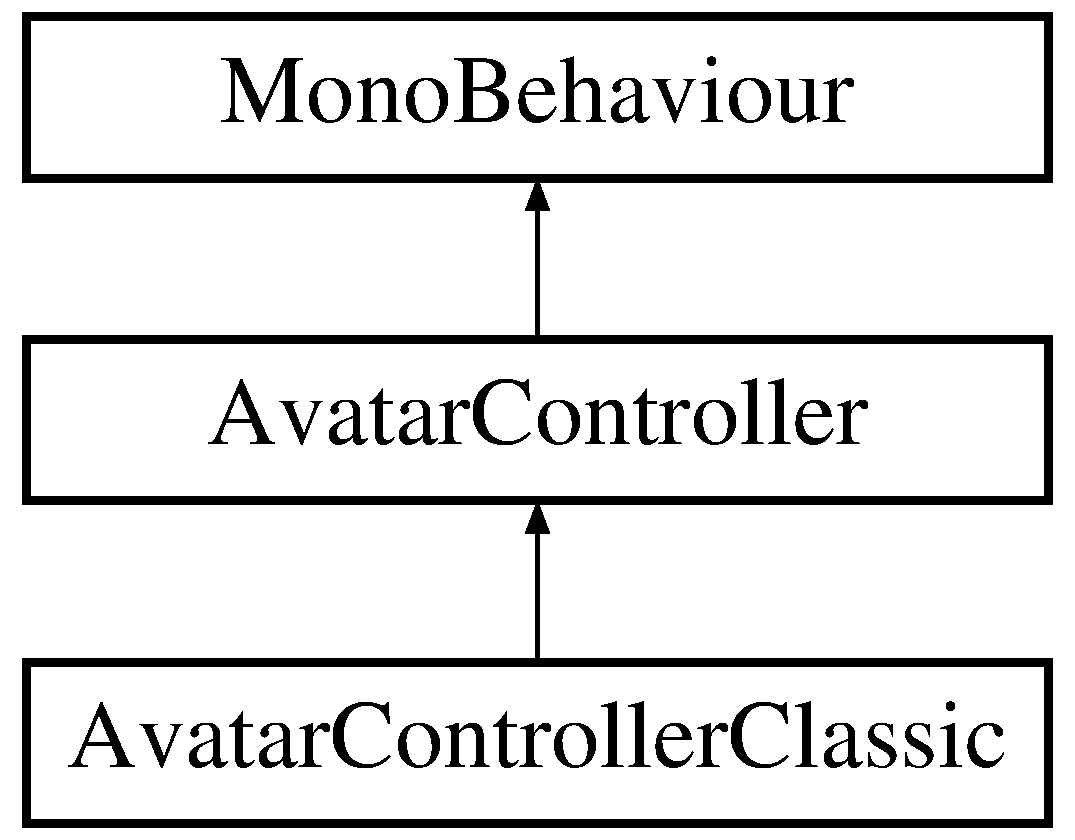
\includegraphics[height=3.000000cm]{class_avatar_controller}
\end{center}
\end{figure}
\subsection*{Public Member Functions}
\begin{DoxyCompactItemize}
\item 
\mbox{\Hypertarget{class_avatar_controller_a6fca9255887e52a99fe05978c26e909f}\label{class_avatar_controller_a6fca9255887e52a99fe05978c26e909f}} 
void {\bfseries Awake} ()
\item 
\mbox{\Hypertarget{class_avatar_controller_ac941da41d7d6f5cf78d8473b660c508a}\label{class_avatar_controller_ac941da41d7d6f5cf78d8473b660c508a}} 
void {\bfseries Update\+Avatar} (uint User\+ID)
\item 
\mbox{\Hypertarget{class_avatar_controller_a4b66eff1306b6dd78a9bc1961c21ff05}\label{class_avatar_controller_a4b66eff1306b6dd78a9bc1961c21ff05}} 
void {\bfseries Reset\+To\+Initial\+Position} ()
\item 
\mbox{\Hypertarget{class_avatar_controller_af22254a125eb1a2e1362e0cde161a3a9}\label{class_avatar_controller_af22254a125eb1a2e1362e0cde161a3a9}} 
void {\bfseries Successful\+Calibration} (uint user\+Id)
\end{DoxyCompactItemize}
\subsection*{Public Attributes}
\begin{DoxyCompactItemize}
\item 
\mbox{\Hypertarget{class_avatar_controller_ae4b12583a22d820211b93b27c0f4019c}\label{class_avatar_controller_ae4b12583a22d820211b93b27c0f4019c}} 
bool {\bfseries mirrored\+Movement} = false
\item 
\mbox{\Hypertarget{class_avatar_controller_ad879ee9629b94cb1c4feaacda6469ba5}\label{class_avatar_controller_ad879ee9629b94cb1c4feaacda6469ba5}} 
bool {\bfseries vertical\+Movement} = false
\item 
\mbox{\Hypertarget{class_avatar_controller_a7a321f1989438d0a77848636a04c4bb5}\label{class_avatar_controller_a7a321f1989438d0a77848636a04c4bb5}} 
float {\bfseries smooth\+Factor} = 5f
\item 
\mbox{\Hypertarget{class_avatar_controller_aa379013fbfd748dc0ccd9ffedfb759d2}\label{class_avatar_controller_aa379013fbfd748dc0ccd9ffedfb759d2}} 
bool {\bfseries offset\+Relative\+To\+Sensor} = false
\end{DoxyCompactItemize}
\subsection*{Protected Member Functions}
\begin{DoxyCompactItemize}
\item 
\mbox{\Hypertarget{class_avatar_controller_affff56fcbd62ebea1efea35ea4a72cb8}\label{class_avatar_controller_affff56fcbd62ebea1efea35ea4a72cb8}} 
void {\bfseries Transform\+Bone} (uint user\+Id, Kinect\+Wrapper.\+Nui\+Skeleton\+Position\+Index joint, int bone\+Index, bool flip)
\item 
\mbox{\Hypertarget{class_avatar_controller_a130066065bf8fc071c24a0d0f0972b95}\label{class_avatar_controller_a130066065bf8fc071c24a0d0f0972b95}} 
void {\bfseries Transform\+Special\+Bone} (uint user\+Id, Kinect\+Wrapper.\+Nui\+Skeleton\+Position\+Index joint, Kinect\+Wrapper.\+Nui\+Skeleton\+Position\+Index joint\+Parent, int bone\+Index, Vector3 base\+Dir, bool flip)
\item 
\mbox{\Hypertarget{class_avatar_controller_a639ea57d58fd646c134b6a39525f39c6}\label{class_avatar_controller_a639ea57d58fd646c134b6a39525f39c6}} 
void {\bfseries Move\+Avatar} (uint User\+ID)
\item 
\mbox{\Hypertarget{class_avatar_controller_a8f8cd1cae328cc38cf52f0e6a74e6c10}\label{class_avatar_controller_a8f8cd1cae328cc38cf52f0e6a74e6c10}} 
virtual void {\bfseries Map\+Bones} ()
\item 
\mbox{\Hypertarget{class_avatar_controller_a6fdb6363fd5dc2dea534889d03df26a7}\label{class_avatar_controller_a6fdb6363fd5dc2dea534889d03df26a7}} 
void {\bfseries Get\+Initial\+Rotations} ()
\item 
\mbox{\Hypertarget{class_avatar_controller_a0946ebc70d224589da85b0e629675fb6}\label{class_avatar_controller_a0946ebc70d224589da85b0e629675fb6}} 
Quaternion {\bfseries Kinect2\+Avatar\+Rot} (Quaternion joint\+Rotation, int bone\+Index)
\item 
\mbox{\Hypertarget{class_avatar_controller_a8e275933bb7c53eb46449bd2aa9680f3}\label{class_avatar_controller_a8e275933bb7c53eb46449bd2aa9680f3}} 
Vector3 {\bfseries Kinect2\+Avatar\+Pos} (Vector3 joint\+Position, bool b\+Move\+Vertically)
\end{DoxyCompactItemize}
\subsection*{Protected Attributes}
\begin{DoxyCompactItemize}
\item 
\mbox{\Hypertarget{class_avatar_controller_aad78a134ad1590839d095803694d91b9}\label{class_avatar_controller_aad78a134ad1590839d095803694d91b9}} 
int {\bfseries move\+Rate} = 1
\item 
\mbox{\Hypertarget{class_avatar_controller_a65abf523bc35b4a09ae3eb3fa4004c96}\label{class_avatar_controller_a65abf523bc35b4a09ae3eb3fa4004c96}} 
Transform {\bfseries body\+Root}
\item 
\mbox{\Hypertarget{class_avatar_controller_abc60dd82fc853ab0749a6d7478dc955e}\label{class_avatar_controller_abc60dd82fc853ab0749a6d7478dc955e}} 
Game\+Object {\bfseries offset\+Node}
\item 
\mbox{\Hypertarget{class_avatar_controller_ae55f16667eb32862ec5fd697e6113439}\label{class_avatar_controller_ae55f16667eb32862ec5fd697e6113439}} 
Transform \mbox{[}$\,$\mbox{]} {\bfseries bones}
\item 
\mbox{\Hypertarget{class_avatar_controller_ae8ec8b3517c912e1945f3c92cc5830c1}\label{class_avatar_controller_ae8ec8b3517c912e1945f3c92cc5830c1}} 
Quaternion \mbox{[}$\,$\mbox{]} {\bfseries initial\+Rotations}
\item 
\mbox{\Hypertarget{class_avatar_controller_a385dc0e8a1b0ab54d97a67fd66741b53}\label{class_avatar_controller_a385dc0e8a1b0ab54d97a67fd66741b53}} 
Quaternion \mbox{[}$\,$\mbox{]} {\bfseries initial\+Local\+Rotations}
\item 
\mbox{\Hypertarget{class_avatar_controller_ac86ce814dd2d6e590ea7f900dc95419f}\label{class_avatar_controller_ac86ce814dd2d6e590ea7f900dc95419f}} 
Vector3 {\bfseries initial\+Position}
\item 
\mbox{\Hypertarget{class_avatar_controller_a3a82b63267763f54d80b16c7caff87b3}\label{class_avatar_controller_a3a82b63267763f54d80b16c7caff87b3}} 
Quaternion {\bfseries initial\+Rotation}
\item 
\mbox{\Hypertarget{class_avatar_controller_a2edd2f991e0dd088a200c9824b6b38b1}\label{class_avatar_controller_a2edd2f991e0dd088a200c9824b6b38b1}} 
bool {\bfseries offset\+Calibrated} = false
\item 
\mbox{\Hypertarget{class_avatar_controller_abba3a50e1e85bebe02f1e9f9861dab6b}\label{class_avatar_controller_abba3a50e1e85bebe02f1e9f9861dab6b}} 
float {\bfseries x\+Offset}
\item 
\mbox{\Hypertarget{class_avatar_controller_a184d57b6eb71497ed7a12ed30eb52bae}\label{class_avatar_controller_a184d57b6eb71497ed7a12ed30eb52bae}} 
\mbox{\hyperlink{class_kinect_manager}{Kinect\+Manager}} {\bfseries kinect\+Manager}
\item 
readonly Dictionary$<$ int, Kinect\+Wrapper.\+Nui\+Skeleton\+Position\+Index $>$ {\bfseries bone\+Index2\+Joint\+Map}
\item 
readonly Dictionary$<$ int, List$<$ Kinect\+Wrapper.\+Nui\+Skeleton\+Position\+Index $>$ $>$ {\bfseries spec\+Index2\+Joint\+Map}
\item 
readonly Dictionary$<$ int, Kinect\+Wrapper.\+Nui\+Skeleton\+Position\+Index $>$ {\bfseries bone\+Index2\+Mirror\+Joint\+Map}
\item 
readonly Dictionary$<$ int, List$<$ Kinect\+Wrapper.\+Nui\+Skeleton\+Position\+Index $>$ $>$ {\bfseries spec\+Index2\+Mirror\+Joint\+Map}
\end{DoxyCompactItemize}
\subsection*{Properties}
\begin{DoxyCompactItemize}
\item 
\mbox{\Hypertarget{class_avatar_controller_a38a4ef1c0030484ba18dd905f850aa7a}\label{class_avatar_controller_a38a4ef1c0030484ba18dd905f850aa7a}} 
new Transform {\bfseries transform}\hspace{0.3cm}{\ttfamily  \mbox{[}get\mbox{]}}
\end{DoxyCompactItemize}


\subsection{Member Data Documentation}
\mbox{\Hypertarget{class_avatar_controller_af44970b84262aacd3c76c192095fedd7}\label{class_avatar_controller_af44970b84262aacd3c76c192095fedd7}} 
\index{Avatar\+Controller@{Avatar\+Controller}!bone\+Index2\+Joint\+Map@{bone\+Index2\+Joint\+Map}}
\index{bone\+Index2\+Joint\+Map@{bone\+Index2\+Joint\+Map}!Avatar\+Controller@{Avatar\+Controller}}
\subsubsection{\texorpdfstring{bone\+Index2\+Joint\+Map}{boneIndex2JointMap}}
{\footnotesize\ttfamily readonly Dictionary$<$int, Kinect\+Wrapper.\+Nui\+Skeleton\+Position\+Index$>$ Avatar\+Controller.\+bone\+Index2\+Joint\+Map\hspace{0.3cm}{\ttfamily [protected]}}

{\bfseries Initial value\+:}
\begin{DoxyCode}
= \textcolor{keyword}{new} Dictionary<int, \mbox{\hyperlink{class_kinect_wrapper}{KinectWrapper}}.NuiSkeletonPositionIndex>
    \{
        \{0, \mbox{\hyperlink{class_kinect_wrapper}{KinectWrapper}}.NuiSkeletonPositionIndex.HipCenter\},
        \{1, \mbox{\hyperlink{class_kinect_wrapper}{KinectWrapper}}.NuiSkeletonPositionIndex.Spine\},
        \{2, \mbox{\hyperlink{class_kinect_wrapper}{KinectWrapper}}.NuiSkeletonPositionIndex.ShoulderCenter\},
        \{3, \mbox{\hyperlink{class_kinect_wrapper}{KinectWrapper}}.NuiSkeletonPositionIndex.Head\},
        
        \{5, \mbox{\hyperlink{class_kinect_wrapper}{KinectWrapper}}.NuiSkeletonPositionIndex.ShoulderLeft\},
        \{6, \mbox{\hyperlink{class_kinect_wrapper}{KinectWrapper}}.NuiSkeletonPositionIndex.ElbowLeft\},
        \{7, \mbox{\hyperlink{class_kinect_wrapper}{KinectWrapper}}.NuiSkeletonPositionIndex.WristLeft\},
        \{8, \mbox{\hyperlink{class_kinect_wrapper}{KinectWrapper}}.NuiSkeletonPositionIndex.HandLeft\},
        
        \{10, \mbox{\hyperlink{class_kinect_wrapper}{KinectWrapper}}.NuiSkeletonPositionIndex.ShoulderRight\},
        \{11, \mbox{\hyperlink{class_kinect_wrapper}{KinectWrapper}}.NuiSkeletonPositionIndex.ElbowRight\},
        \{12, \mbox{\hyperlink{class_kinect_wrapper}{KinectWrapper}}.NuiSkeletonPositionIndex.WristRight\},
        \{13, \mbox{\hyperlink{class_kinect_wrapper}{KinectWrapper}}.NuiSkeletonPositionIndex.HandRight\},
        
        \{14, \mbox{\hyperlink{class_kinect_wrapper}{KinectWrapper}}.NuiSkeletonPositionIndex.HipLeft\},
        \{15, \mbox{\hyperlink{class_kinect_wrapper}{KinectWrapper}}.NuiSkeletonPositionIndex.KneeLeft\},
        \{16, \mbox{\hyperlink{class_kinect_wrapper}{KinectWrapper}}.NuiSkeletonPositionIndex.AnkleLeft\},
        \{17, \mbox{\hyperlink{class_kinect_wrapper}{KinectWrapper}}.NuiSkeletonPositionIndex.FootLeft\},
        
        \{18, \mbox{\hyperlink{class_kinect_wrapper}{KinectWrapper}}.NuiSkeletonPositionIndex.HipRight\},
        \{19, \mbox{\hyperlink{class_kinect_wrapper}{KinectWrapper}}.NuiSkeletonPositionIndex.KneeRight\},
        \{20, \mbox{\hyperlink{class_kinect_wrapper}{KinectWrapper}}.NuiSkeletonPositionIndex.AnkleRight\},
        \{21, \mbox{\hyperlink{class_kinect_wrapper}{KinectWrapper}}.NuiSkeletonPositionIndex.FootRight\},
    \}
\end{DoxyCode}
\mbox{\Hypertarget{class_avatar_controller_acf75b54900c0f65fcd27d9a998582ef8}\label{class_avatar_controller_acf75b54900c0f65fcd27d9a998582ef8}} 
\index{Avatar\+Controller@{Avatar\+Controller}!bone\+Index2\+Mirror\+Joint\+Map@{bone\+Index2\+Mirror\+Joint\+Map}}
\index{bone\+Index2\+Mirror\+Joint\+Map@{bone\+Index2\+Mirror\+Joint\+Map}!Avatar\+Controller@{Avatar\+Controller}}
\subsubsection{\texorpdfstring{bone\+Index2\+Mirror\+Joint\+Map}{boneIndex2MirrorJointMap}}
{\footnotesize\ttfamily readonly Dictionary$<$int, Kinect\+Wrapper.\+Nui\+Skeleton\+Position\+Index$>$ Avatar\+Controller.\+bone\+Index2\+Mirror\+Joint\+Map\hspace{0.3cm}{\ttfamily [protected]}}

{\bfseries Initial value\+:}
\begin{DoxyCode}
= \textcolor{keyword}{new} Dictionary<int, \mbox{\hyperlink{class_kinect_wrapper}{KinectWrapper}}.NuiSkeletonPositionIndex>
    \{
        \{0, \mbox{\hyperlink{class_kinect_wrapper}{KinectWrapper}}.NuiSkeletonPositionIndex.HipCenter\},
        \{1, \mbox{\hyperlink{class_kinect_wrapper}{KinectWrapper}}.NuiSkeletonPositionIndex.Spine\},
        \{2, \mbox{\hyperlink{class_kinect_wrapper}{KinectWrapper}}.NuiSkeletonPositionIndex.ShoulderCenter\},
        \{3, \mbox{\hyperlink{class_kinect_wrapper}{KinectWrapper}}.NuiSkeletonPositionIndex.Head\},
        
        \{5, \mbox{\hyperlink{class_kinect_wrapper}{KinectWrapper}}.NuiSkeletonPositionIndex.ShoulderRight\},
        \{6, \mbox{\hyperlink{class_kinect_wrapper}{KinectWrapper}}.NuiSkeletonPositionIndex.ElbowRight\},
        \{7, \mbox{\hyperlink{class_kinect_wrapper}{KinectWrapper}}.NuiSkeletonPositionIndex.WristRight\},
        \{8, \mbox{\hyperlink{class_kinect_wrapper}{KinectWrapper}}.NuiSkeletonPositionIndex.HandRight\},
        
        \{10, \mbox{\hyperlink{class_kinect_wrapper}{KinectWrapper}}.NuiSkeletonPositionIndex.ShoulderLeft\},
        \{11, \mbox{\hyperlink{class_kinect_wrapper}{KinectWrapper}}.NuiSkeletonPositionIndex.ElbowLeft\},
        \{12, \mbox{\hyperlink{class_kinect_wrapper}{KinectWrapper}}.NuiSkeletonPositionIndex.WristLeft\},
        \{13, \mbox{\hyperlink{class_kinect_wrapper}{KinectWrapper}}.NuiSkeletonPositionIndex.HandLeft\},
        
        \{14, \mbox{\hyperlink{class_kinect_wrapper}{KinectWrapper}}.NuiSkeletonPositionIndex.HipRight\},
        \{15, \mbox{\hyperlink{class_kinect_wrapper}{KinectWrapper}}.NuiSkeletonPositionIndex.KneeRight\},
        \{16, \mbox{\hyperlink{class_kinect_wrapper}{KinectWrapper}}.NuiSkeletonPositionIndex.AnkleRight\},
        \{17, \mbox{\hyperlink{class_kinect_wrapper}{KinectWrapper}}.NuiSkeletonPositionIndex.FootRight\},
        
        \{18, \mbox{\hyperlink{class_kinect_wrapper}{KinectWrapper}}.NuiSkeletonPositionIndex.HipLeft\},
        \{19, \mbox{\hyperlink{class_kinect_wrapper}{KinectWrapper}}.NuiSkeletonPositionIndex.KneeLeft\},
        \{20, \mbox{\hyperlink{class_kinect_wrapper}{KinectWrapper}}.NuiSkeletonPositionIndex.AnkleLeft\},
        \{21, \mbox{\hyperlink{class_kinect_wrapper}{KinectWrapper}}.NuiSkeletonPositionIndex.FootLeft\},
    \}
\end{DoxyCode}
\mbox{\Hypertarget{class_avatar_controller_a8143c80aaad868c53ca674b41759d82b}\label{class_avatar_controller_a8143c80aaad868c53ca674b41759d82b}} 
\index{Avatar\+Controller@{Avatar\+Controller}!spec\+Index2\+Joint\+Map@{spec\+Index2\+Joint\+Map}}
\index{spec\+Index2\+Joint\+Map@{spec\+Index2\+Joint\+Map}!Avatar\+Controller@{Avatar\+Controller}}
\subsubsection{\texorpdfstring{spec\+Index2\+Joint\+Map}{specIndex2JointMap}}
{\footnotesize\ttfamily readonly Dictionary$<$int, List$<$Kinect\+Wrapper.\+Nui\+Skeleton\+Position\+Index$>$ $>$ Avatar\+Controller.\+spec\+Index2\+Joint\+Map\hspace{0.3cm}{\ttfamily [protected]}}

{\bfseries Initial value\+:}
\begin{DoxyCode}
= \textcolor{keyword}{new} Dictionary<int, List<\mbox{\hyperlink{class_kinect_wrapper}{KinectWrapper}}.NuiSkeletonPositionIndex>>
    \{
        \{4, \textcolor{keyword}{new} List<\mbox{\hyperlink{class_kinect_wrapper}{KinectWrapper}}.NuiSkeletonPositionIndex> \{
      \mbox{\hyperlink{class_kinect_wrapper}{KinectWrapper}}.NuiSkeletonPositionIndex.ShoulderLeft, \mbox{\hyperlink{class_kinect_wrapper}{KinectWrapper}}.
      NuiSkeletonPositionIndex.ShoulderCenter\} \},
        \{9, \textcolor{keyword}{new} List<\mbox{\hyperlink{class_kinect_wrapper}{KinectWrapper}}.NuiSkeletonPositionIndex> \{
      \mbox{\hyperlink{class_kinect_wrapper}{KinectWrapper}}.NuiSkeletonPositionIndex.ShoulderRight, \mbox{\hyperlink{class_kinect_wrapper}{KinectWrapper}}.
      NuiSkeletonPositionIndex.ShoulderCenter\} \},
    \}
\end{DoxyCode}
\mbox{\Hypertarget{class_avatar_controller_ad954ba1369590ca3534bd206eb8bd72a}\label{class_avatar_controller_ad954ba1369590ca3534bd206eb8bd72a}} 
\index{Avatar\+Controller@{Avatar\+Controller}!spec\+Index2\+Mirror\+Joint\+Map@{spec\+Index2\+Mirror\+Joint\+Map}}
\index{spec\+Index2\+Mirror\+Joint\+Map@{spec\+Index2\+Mirror\+Joint\+Map}!Avatar\+Controller@{Avatar\+Controller}}
\subsubsection{\texorpdfstring{spec\+Index2\+Mirror\+Joint\+Map}{specIndex2MirrorJointMap}}
{\footnotesize\ttfamily readonly Dictionary$<$int, List$<$Kinect\+Wrapper.\+Nui\+Skeleton\+Position\+Index$>$ $>$ Avatar\+Controller.\+spec\+Index2\+Mirror\+Joint\+Map\hspace{0.3cm}{\ttfamily [protected]}}

{\bfseries Initial value\+:}
\begin{DoxyCode}
= \textcolor{keyword}{new} Dictionary<int, List<\mbox{\hyperlink{class_kinect_wrapper}{KinectWrapper}}.NuiSkeletonPositionIndex>>
    \{
        \{4, \textcolor{keyword}{new} List<\mbox{\hyperlink{class_kinect_wrapper}{KinectWrapper}}.NuiSkeletonPositionIndex> \{
      \mbox{\hyperlink{class_kinect_wrapper}{KinectWrapper}}.NuiSkeletonPositionIndex.ShoulderRight, \mbox{\hyperlink{class_kinect_wrapper}{KinectWrapper}}.
      NuiSkeletonPositionIndex.ShoulderCenter\} \},
        \{9, \textcolor{keyword}{new} List<\mbox{\hyperlink{class_kinect_wrapper}{KinectWrapper}}.NuiSkeletonPositionIndex> \{
      \mbox{\hyperlink{class_kinect_wrapper}{KinectWrapper}}.NuiSkeletonPositionIndex.ShoulderLeft, \mbox{\hyperlink{class_kinect_wrapper}{KinectWrapper}}.
      NuiSkeletonPositionIndex.ShoulderCenter\} \},
    \}
\end{DoxyCode}


The documentation for this class was generated from the following file\+:\begin{DoxyCompactItemize}
\item 
Assets/\+Kinect\+Scripts/Avatar\+Controller.\+cs\end{DoxyCompactItemize}

\hypertarget{class_avatar_controller_classic}{}\section{Avatar\+Controller\+Classic Class Reference}
\label{class_avatar_controller_classic}\index{Avatar\+Controller\+Classic@{Avatar\+Controller\+Classic}}
Inheritance diagram for Avatar\+Controller\+Classic\+:\begin{figure}[H]
\begin{center}
\leavevmode
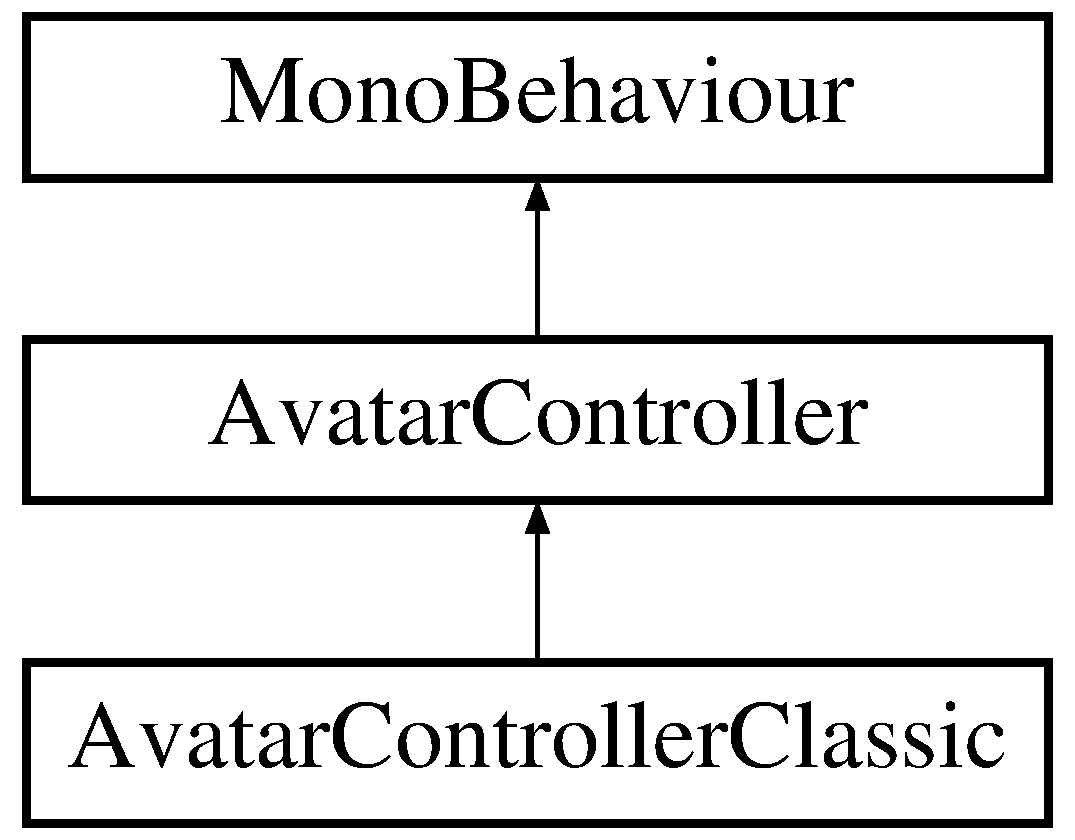
\includegraphics[height=3.000000cm]{class_avatar_controller_classic}
\end{center}
\end{figure}
\subsection*{Public Attributes}
\begin{DoxyCompactItemize}
\item 
\mbox{\Hypertarget{class_avatar_controller_classic_a97381312097be4061e4c96bbe4ba3e68}\label{class_avatar_controller_classic_a97381312097be4061e4c96bbe4ba3e68}} 
Transform {\bfseries Hip\+Center}
\item 
\mbox{\Hypertarget{class_avatar_controller_classic_a075622ff023b9e9aa3a46ceeb9282ffe}\label{class_avatar_controller_classic_a075622ff023b9e9aa3a46ceeb9282ffe}} 
Transform {\bfseries Spine}
\item 
\mbox{\Hypertarget{class_avatar_controller_classic_a8240504305f3cdd3f0d43e26cfb36a94}\label{class_avatar_controller_classic_a8240504305f3cdd3f0d43e26cfb36a94}} 
Transform {\bfseries Neck}
\item 
\mbox{\Hypertarget{class_avatar_controller_classic_ae18ccea555fb7f7735be2c3e70b838ab}\label{class_avatar_controller_classic_ae18ccea555fb7f7735be2c3e70b838ab}} 
Transform {\bfseries Head}
\item 
\mbox{\Hypertarget{class_avatar_controller_classic_a27dfc8720c4d0e7791103006553b2105}\label{class_avatar_controller_classic_a27dfc8720c4d0e7791103006553b2105}} 
Transform {\bfseries Left\+Clavicle}
\item 
\mbox{\Hypertarget{class_avatar_controller_classic_a904c745cc61cb00ee96c5e4a0d70eb0d}\label{class_avatar_controller_classic_a904c745cc61cb00ee96c5e4a0d70eb0d}} 
Transform {\bfseries Left\+Upper\+Arm}
\item 
\mbox{\Hypertarget{class_avatar_controller_classic_a7bebf9c22e08032075e528608a04d7b8}\label{class_avatar_controller_classic_a7bebf9c22e08032075e528608a04d7b8}} 
Transform {\bfseries Left\+Elbow}
\item 
\mbox{\Hypertarget{class_avatar_controller_classic_af812998e9e13fbfc61850c1cc6a1c131}\label{class_avatar_controller_classic_af812998e9e13fbfc61850c1cc6a1c131}} 
Transform {\bfseries Left\+Hand}
\item 
\mbox{\Hypertarget{class_avatar_controller_classic_adf0861da2392d2985b40dc5f38e15d76}\label{class_avatar_controller_classic_adf0861da2392d2985b40dc5f38e15d76}} 
Transform {\bfseries Right\+Clavicle}
\item 
\mbox{\Hypertarget{class_avatar_controller_classic_a3c6d49c333ed48a0fbf0886519e8a85d}\label{class_avatar_controller_classic_a3c6d49c333ed48a0fbf0886519e8a85d}} 
Transform {\bfseries Right\+Upper\+Arm}
\item 
\mbox{\Hypertarget{class_avatar_controller_classic_a0cf9155892c5c20e4325fa60d7bd6c93}\label{class_avatar_controller_classic_a0cf9155892c5c20e4325fa60d7bd6c93}} 
Transform {\bfseries Right\+Elbow}
\item 
\mbox{\Hypertarget{class_avatar_controller_classic_ab04e972e968066bbe478b6dafb6cd5cc}\label{class_avatar_controller_classic_ab04e972e968066bbe478b6dafb6cd5cc}} 
Transform {\bfseries Right\+Hand}
\item 
\mbox{\Hypertarget{class_avatar_controller_classic_abdaa0f6fcfdba8732ae3a8ca755b701c}\label{class_avatar_controller_classic_abdaa0f6fcfdba8732ae3a8ca755b701c}} 
Transform {\bfseries Left\+Thigh}
\item 
\mbox{\Hypertarget{class_avatar_controller_classic_a2d69632d51cfde22f2f079fe22377b4c}\label{class_avatar_controller_classic_a2d69632d51cfde22f2f079fe22377b4c}} 
Transform {\bfseries Left\+Knee}
\item 
\mbox{\Hypertarget{class_avatar_controller_classic_a1309a404f5eb0e6f490b34c478ae6a4a}\label{class_avatar_controller_classic_a1309a404f5eb0e6f490b34c478ae6a4a}} 
Transform {\bfseries Left\+Foot}
\item 
\mbox{\Hypertarget{class_avatar_controller_classic_a7f2e10dd1348f43424b0643069aa65d5}\label{class_avatar_controller_classic_a7f2e10dd1348f43424b0643069aa65d5}} 
Transform {\bfseries Right\+Thigh}
\item 
\mbox{\Hypertarget{class_avatar_controller_classic_a855339b88da04039c0ac16c948a6a9f3}\label{class_avatar_controller_classic_a855339b88da04039c0ac16c948a6a9f3}} 
Transform {\bfseries Right\+Knee}
\item 
\mbox{\Hypertarget{class_avatar_controller_classic_a6716f886168649b4e4e9802cc0e00a3b}\label{class_avatar_controller_classic_a6716f886168649b4e4e9802cc0e00a3b}} 
Transform {\bfseries Right\+Foot}
\item 
\mbox{\Hypertarget{class_avatar_controller_classic_a1c5bc5fe7afb26d985a137698c60fa70}\label{class_avatar_controller_classic_a1c5bc5fe7afb26d985a137698c60fa70}} 
Transform {\bfseries Body\+Root}
\item 
\mbox{\Hypertarget{class_avatar_controller_classic_aaf423bc11650d0bc49fd8fe6266c94ad}\label{class_avatar_controller_classic_aaf423bc11650d0bc49fd8fe6266c94ad}} 
Game\+Object {\bfseries Offset\+Node}
\end{DoxyCompactItemize}
\subsection*{Protected Member Functions}
\begin{DoxyCompactItemize}
\item 
\mbox{\Hypertarget{class_avatar_controller_classic_a2f29066ac96cf8bcd12a8c2c982e0c17}\label{class_avatar_controller_classic_a2f29066ac96cf8bcd12a8c2c982e0c17}} 
override void {\bfseries Map\+Bones} ()
\end{DoxyCompactItemize}
\subsection*{Additional Inherited Members}


The documentation for this class was generated from the following file\+:\begin{DoxyCompactItemize}
\item 
Assets/\+Kinect\+Scripts/Avatar\+Controller\+Classic.\+cs\end{DoxyCompactItemize}

\hypertarget{class_bone_orientations_constraint}{}\section{Bone\+Orientations\+Constraint Class Reference}
\label{class_bone_orientations_constraint}\index{Bone\+Orientations\+Constraint@{Bone\+Orientations\+Constraint}}


Filter to correct the joint locations and joint orientations to constraint to range of viable human motion.  


\subsection*{Public Types}
\begin{DoxyCompactItemize}
\item 
\mbox{\Hypertarget{class_bone_orientations_constraint_a1f4aa21ffa8dbc27a16143698d71e63d}\label{class_bone_orientations_constraint_a1f4aa21ffa8dbc27a16143698d71e63d}} 
enum {\bfseries Constraint\+Axis} \{ {\bfseries X} = 0, 
{\bfseries Y} = 1, 
{\bfseries Z} = 2
 \}
\end{DoxyCompactItemize}
\subsection*{Public Member Functions}
\begin{DoxyCompactItemize}
\item 
\mbox{\Hypertarget{class_bone_orientations_constraint_a8f9232ef89117f7a5ea6977acf5ce622}\label{class_bone_orientations_constraint_a8f9232ef89117f7a5ea6977acf5ce622}} 
\mbox{\hyperlink{class_bone_orientations_constraint_a8f9232ef89117f7a5ea6977acf5ce622}{Bone\+Orientations\+Constraint}} ()
\begin{DoxyCompactList}\small\item\em Initializes a new instance of the Bone\+Orientation\+Constraints class. \end{DoxyCompactList}\item 
\mbox{\Hypertarget{class_bone_orientations_constraint_ab9dcd6608443e194a4c3a098baec5138}\label{class_bone_orientations_constraint_ab9dcd6608443e194a4c3a098baec5138}} 
void {\bfseries Add\+Bone\+Orientation\+Constraint} (int joint, Constraint\+Axis axis, float angle\+Min, float angle\+Max)
\item 
\mbox{\Hypertarget{class_bone_orientations_constraint_a9c6fb36deaa012c5ca393200ed273986}\label{class_bone_orientations_constraint_a9c6fb36deaa012c5ca393200ed273986}} 
void {\bfseries Add\+Default\+Constraints} ()
\item 
\mbox{\Hypertarget{class_bone_orientations_constraint_a8387f8886926069be888c2aca2ddb1e8}\label{class_bone_orientations_constraint_a8387f8886926069be888c2aca2ddb1e8}} 
void {\bfseries Constrain} (ref Matrix4x4\mbox{[}$\,$\mbox{]} joint\+Orientations, ref bool\mbox{[}$\,$\mbox{]} joint\+Tracked)
\end{DoxyCompactItemize}


\subsection{Detailed Description}
Filter to correct the joint locations and joint orientations to constraint to range of viable human motion. 



The documentation for this class was generated from the following file\+:\begin{DoxyCompactItemize}
\item 
Assets/\+Kinect\+Scripts/\+Filters/Bone\+Orientations\+Constraint.\+cs\end{DoxyCompactItemize}

\hypertarget{class_bone_orientations_filter}{}\section{Bone\+Orientations\+Filter Class Reference}
\label{class_bone_orientations_filter}\index{Bone\+Orientations\+Filter@{Bone\+Orientations\+Filter}}


Implementation of a Holt Double Exponential Smoothing filter for orientation. The double exponential smooths the curve and predicts. There is also noise jitter removal. And maximum prediction bounds. The parameters are commented in the Init function.  


\subsection*{Public Member Functions}
\begin{DoxyCompactItemize}
\item 
\mbox{\Hypertarget{class_bone_orientations_filter_a3be769b3d49e677fa475b6d7d3de5f52}\label{class_bone_orientations_filter_a3be769b3d49e677fa475b6d7d3de5f52}} 
void {\bfseries Init} ()
\item 
void \mbox{\hyperlink{class_bone_orientations_filter_a0cfdcfa52dc01bac029c04084dca64f2}{Init}} (float smoothing\+Value, float correction\+Value, float prediction\+Value, float jitter\+Radius\+Value, float max\+Deviation\+Radius\+Value)
\begin{DoxyCompactList}\small\item\em Initialize the filter with a set of manually specified Transform\+Smooth\+Parameters. \end{DoxyCompactList}\item 
\mbox{\Hypertarget{class_bone_orientations_filter_ae7531e45a6afef3e56cfe6a857cfccf4}\label{class_bone_orientations_filter_ae7531e45a6afef3e56cfe6a857cfccf4}} 
void {\bfseries Init} (\mbox{\hyperlink{struct_kinect_wrapper_1_1_nui_transform_smooth_parameters}{Kinect\+Wrapper.\+Nui\+Transform\+Smooth\+Parameters}} smoothing\+Parameters)
\item 
\mbox{\Hypertarget{class_bone_orientations_filter_a7460b686bf3641385a9e09725ae146df}\label{class_bone_orientations_filter_a7460b686bf3641385a9e09725ae146df}} 
void \mbox{\hyperlink{class_bone_orientations_filter_a7460b686bf3641385a9e09725ae146df}{Reset}} ()
\begin{DoxyCompactList}\small\item\em Resets the filter to default values. \end{DoxyCompactList}\item 
\mbox{\Hypertarget{class_bone_orientations_filter_a0f170cd9ad67f29a62688afa09916560}\label{class_bone_orientations_filter_a0f170cd9ad67f29a62688afa09916560}} 
void {\bfseries Update\+Filter} (ref \mbox{\hyperlink{struct_kinect_wrapper_1_1_nui_skeleton_data}{Kinect\+Wrapper.\+Nui\+Skeleton\+Data}} skeleton, ref Matrix4x4\mbox{[}$\,$\mbox{]} joint\+Orientations)
\end{DoxyCompactItemize}
\subsection*{Protected Member Functions}
\begin{DoxyCompactItemize}
\item 
\mbox{\Hypertarget{class_bone_orientations_filter_a9a5af74c297bb1815b24932aa6895786}\label{class_bone_orientations_filter_a9a5af74c297bb1815b24932aa6895786}} 
void {\bfseries Filter\+Joint} (ref \mbox{\hyperlink{struct_kinect_wrapper_1_1_nui_skeleton_data}{Kinect\+Wrapper.\+Nui\+Skeleton\+Data}} skeleton, int joint\+Index, ref \mbox{\hyperlink{struct_kinect_wrapper_1_1_nui_transform_smooth_parameters}{Kinect\+Wrapper.\+Nui\+Transform\+Smooth\+Parameters}} smoothing\+Parameters, ref Matrix4x4\mbox{[}$\,$\mbox{]} joint\+Orientations)
\end{DoxyCompactItemize}


\subsection{Detailed Description}
Implementation of a Holt Double Exponential Smoothing filter for orientation. The double exponential smooths the curve and predicts. There is also noise jitter removal. And maximum prediction bounds. The parameters are commented in the Init function. 



\subsection{Member Function Documentation}
\mbox{\Hypertarget{class_bone_orientations_filter_a0cfdcfa52dc01bac029c04084dca64f2}\label{class_bone_orientations_filter_a0cfdcfa52dc01bac029c04084dca64f2}} 
\index{Bone\+Orientations\+Filter@{Bone\+Orientations\+Filter}!Init@{Init}}
\index{Init@{Init}!Bone\+Orientations\+Filter@{Bone\+Orientations\+Filter}}
\subsubsection{\texorpdfstring{Init()}{Init()}}
{\footnotesize\ttfamily void Bone\+Orientations\+Filter.\+Init (\begin{DoxyParamCaption}\item[{float}]{smoothing\+Value,  }\item[{float}]{correction\+Value,  }\item[{float}]{prediction\+Value,  }\item[{float}]{jitter\+Radius\+Value,  }\item[{float}]{max\+Deviation\+Radius\+Value }\end{DoxyParamCaption})}



Initialize the filter with a set of manually specified Transform\+Smooth\+Parameters. 


\begin{DoxyParams}{Parameters}
{\em smoothing\+Value} & Smoothing = \mbox{[}0..1\mbox{]}, lower values is closer to the raw data and more noisy.\\
\hline
{\em correction\+Value} & Correction = \mbox{[}0..1\mbox{]}, higher values correct faster and feel more responsive.\\
\hline
{\em prediction\+Value} & Prediction = \mbox{[}0..n\mbox{]}, how many frames into the future we want to predict.\\
\hline
{\em jitter\+Radius\+Value} & Jitter\+Radius = The deviation angle in radians that defines jitter.\\
\hline
{\em max\+Deviation\+Radius\+Value} & Max\+Deviation = The maximum angle in radians that filtered positions are allowed to deviate from raw data.\\
\hline
\end{DoxyParams}


The documentation for this class was generated from the following file\+:\begin{DoxyCompactItemize}
\item 
Assets/\+Kinect\+Scripts/\+Filters/Bone\+Orientations\+Filter.\+cs\end{DoxyCompactItemize}

\hypertarget{class_clipped_legs_filter}{}\section{Clipped\+Legs\+Filter Class Reference}
\label{class_clipped_legs_filter}\index{Clipped\+Legs\+Filter@{Clipped\+Legs\+Filter}}


Filter\+Clipped\+Legs smooths out leg joint positions when the skeleton is clipped by the bottom of the camera F\+OV. Inferred joint positions from the skeletal tracker can occasionally be noisy or erroneous, based on limited depth image pixels from the parts of the legs in view. This filter applies a lot of smoothing using a double exponential filter, letting through just enough leg movement to show a kick or high step. Based on the amount of leg that is clipped/inferred, the smoothed data is feathered into the skeleton output data.  


\subsection*{Public Member Functions}
\begin{DoxyCompactItemize}
\item 
\mbox{\Hypertarget{class_clipped_legs_filter_a8e0b851496095353a058f36677ec861c}\label{class_clipped_legs_filter_a8e0b851496095353a058f36677ec861c}} 
void {\bfseries Reset} ()
\item 
\mbox{\Hypertarget{class_clipped_legs_filter_a044676e1e38b65570dc9fd47c7394317}\label{class_clipped_legs_filter_a044676e1e38b65570dc9fd47c7394317}} 
bool {\bfseries Filter\+Skeleton} (ref \mbox{\hyperlink{struct_kinect_wrapper_1_1_nui_skeleton_data}{Kinect\+Wrapper.\+Nui\+Skeleton\+Data}} skeleton, float delta\+Nui\+Time)
\end{DoxyCompactItemize}


\subsection{Detailed Description}
Filter\+Clipped\+Legs smooths out leg joint positions when the skeleton is clipped by the bottom of the camera F\+OV. Inferred joint positions from the skeletal tracker can occasionally be noisy or erroneous, based on limited depth image pixels from the parts of the legs in view. This filter applies a lot of smoothing using a double exponential filter, letting through just enough leg movement to show a kick or high step. Based on the amount of leg that is clipped/inferred, the smoothed data is feathered into the skeleton output data. 



The documentation for this class was generated from the following file\+:\begin{DoxyCompactItemize}
\item 
Assets/\+Kinect\+Scripts/\+Filters/Clipped\+Legs\+Filter.\+cs\end{DoxyCompactItemize}

\hypertarget{struct_kinect_wrapper_1_1_color_buffer}{}\section{Kinect\+Wrapper.\+Color\+Buffer Struct Reference}
\label{struct_kinect_wrapper_1_1_color_buffer}\index{Kinect\+Wrapper.\+Color\+Buffer@{Kinect\+Wrapper.\+Color\+Buffer}}
\subsection*{Public Attributes}
\begin{DoxyCompactItemize}
\item 
\mbox{\Hypertarget{struct_kinect_wrapper_1_1_color_buffer_af6c7fc494c351d8092b1020098fa4816}\label{struct_kinect_wrapper_1_1_color_buffer_af6c7fc494c351d8092b1020098fa4816}} 
\mbox{\hyperlink{struct_kinect_wrapper_1_1_color_cust}{Color\+Cust}} \mbox{[}$\,$\mbox{]} {\bfseries pixels}
\end{DoxyCompactItemize}


The documentation for this struct was generated from the following file\+:\begin{DoxyCompactItemize}
\item 
Assets/\+Kinect\+Scripts/Kinect\+Wrapper.\+cs\end{DoxyCompactItemize}

\hypertarget{struct_kinect_wrapper_1_1_color_cust}{}\section{Kinect\+Wrapper.\+Color\+Cust Struct Reference}
\label{struct_kinect_wrapper_1_1_color_cust}\index{Kinect\+Wrapper.\+Color\+Cust@{Kinect\+Wrapper.\+Color\+Cust}}
\subsection*{Public Attributes}
\begin{DoxyCompactItemize}
\item 
\mbox{\Hypertarget{struct_kinect_wrapper_1_1_color_cust_aff71e744cf6de415836b84af52d3025f}\label{struct_kinect_wrapper_1_1_color_cust_aff71e744cf6de415836b84af52d3025f}} 
byte {\bfseries b}
\item 
\mbox{\Hypertarget{struct_kinect_wrapper_1_1_color_cust_abe8b552fcc9ad59a6d8565d14499e898}\label{struct_kinect_wrapper_1_1_color_cust_abe8b552fcc9ad59a6d8565d14499e898}} 
byte {\bfseries g}
\item 
\mbox{\Hypertarget{struct_kinect_wrapper_1_1_color_cust_a398cec0bca93e27ba4335267df2a0cda}\label{struct_kinect_wrapper_1_1_color_cust_a398cec0bca93e27ba4335267df2a0cda}} 
byte {\bfseries r}
\item 
\mbox{\Hypertarget{struct_kinect_wrapper_1_1_color_cust_a662e6b987c8d9d7971faaa131f165aa0}\label{struct_kinect_wrapper_1_1_color_cust_a662e6b987c8d9d7971faaa131f165aa0}} 
byte {\bfseries a}
\end{DoxyCompactItemize}


The documentation for this struct was generated from the following file\+:\begin{DoxyCompactItemize}
\item 
Assets/\+Kinect\+Scripts/Kinect\+Wrapper.\+cs\end{DoxyCompactItemize}

\hypertarget{class_cubeman_controller}{}\section{Cubeman\+Controller Class Reference}
\label{class_cubeman_controller}\index{Cubeman\+Controller@{Cubeman\+Controller}}
Inheritance diagram for Cubeman\+Controller\+:\begin{figure}[H]
\begin{center}
\leavevmode
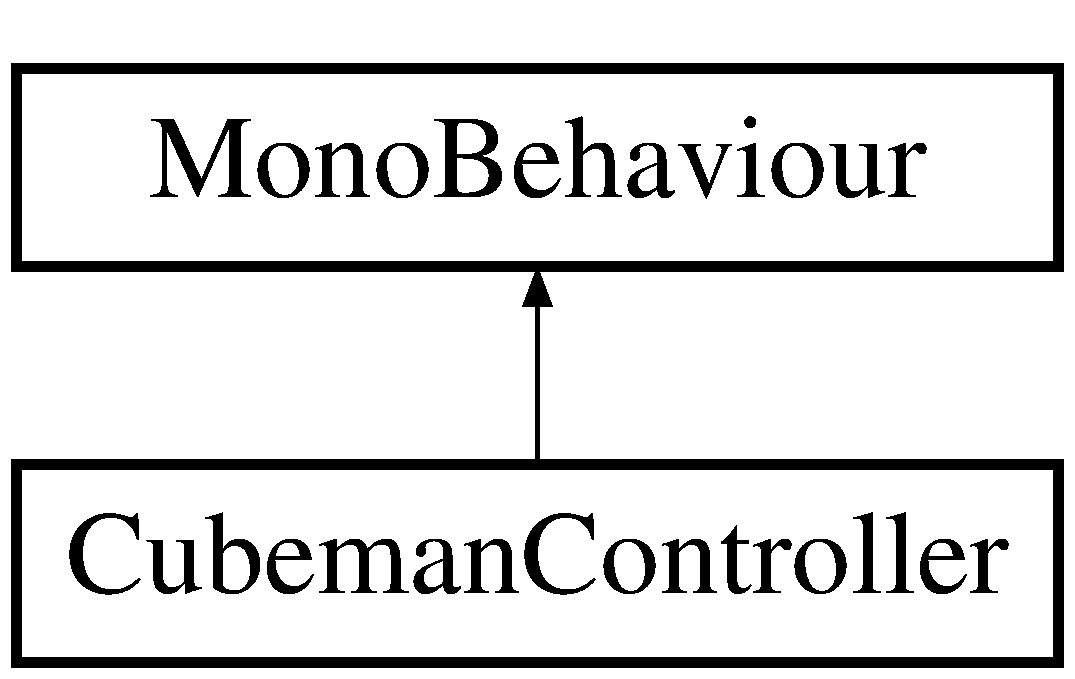
\includegraphics[height=2.000000cm]{class_cubeman_controller}
\end{center}
\end{figure}
\subsection*{Public Attributes}
\begin{DoxyCompactItemize}
\item 
\mbox{\Hypertarget{class_cubeman_controller_a720b4ce57a18e8562f51dc432f241de6}\label{class_cubeman_controller_a720b4ce57a18e8562f51dc432f241de6}} 
bool {\bfseries Move\+Vertically} = false
\item 
\mbox{\Hypertarget{class_cubeman_controller_abaf470777494790dde40d278d9bdc2ed}\label{class_cubeman_controller_abaf470777494790dde40d278d9bdc2ed}} 
bool {\bfseries Mirrored\+Movement} = false
\item 
\mbox{\Hypertarget{class_cubeman_controller_a640866fa9954109f89ac8e6d18d8f21a}\label{class_cubeman_controller_a640866fa9954109f89ac8e6d18d8f21a}} 
Game\+Object {\bfseries Hip\+\_\+\+Center}
\item 
\mbox{\Hypertarget{class_cubeman_controller_a3ee406ee6cfb60eaff989d75968db021}\label{class_cubeman_controller_a3ee406ee6cfb60eaff989d75968db021}} 
Game\+Object {\bfseries Spine}
\item 
\mbox{\Hypertarget{class_cubeman_controller_a9ec367ae7d6a4f3f5b916f800790b104}\label{class_cubeman_controller_a9ec367ae7d6a4f3f5b916f800790b104}} 
Game\+Object {\bfseries Shoulder\+\_\+\+Center}
\item 
\mbox{\Hypertarget{class_cubeman_controller_a01a187776dece60ae5b10452eb63c0be}\label{class_cubeman_controller_a01a187776dece60ae5b10452eb63c0be}} 
Game\+Object {\bfseries Head}
\item 
\mbox{\Hypertarget{class_cubeman_controller_a167626134e677db40c79f3feb24797a3}\label{class_cubeman_controller_a167626134e677db40c79f3feb24797a3}} 
Game\+Object {\bfseries Shoulder\+\_\+\+Left}
\item 
\mbox{\Hypertarget{class_cubeman_controller_aa878f156d1d0adb03e7889f0373d9f5f}\label{class_cubeman_controller_aa878f156d1d0adb03e7889f0373d9f5f}} 
Game\+Object {\bfseries Elbow\+\_\+\+Left}
\item 
\mbox{\Hypertarget{class_cubeman_controller_a50f95ad09b7799eab50e436332d68290}\label{class_cubeman_controller_a50f95ad09b7799eab50e436332d68290}} 
Game\+Object {\bfseries Wrist\+\_\+\+Left}
\item 
\mbox{\Hypertarget{class_cubeman_controller_a963f30db9c453565b36e630a3ddb56e4}\label{class_cubeman_controller_a963f30db9c453565b36e630a3ddb56e4}} 
Game\+Object {\bfseries Hand\+\_\+\+Left}
\item 
\mbox{\Hypertarget{class_cubeman_controller_ae37497dce80b3cae3768f4311a840ccf}\label{class_cubeman_controller_ae37497dce80b3cae3768f4311a840ccf}} 
Game\+Object {\bfseries Shoulder\+\_\+\+Right}
\item 
\mbox{\Hypertarget{class_cubeman_controller_a9f214d7876636e1769013801050c37fa}\label{class_cubeman_controller_a9f214d7876636e1769013801050c37fa}} 
Game\+Object {\bfseries Elbow\+\_\+\+Right}
\item 
\mbox{\Hypertarget{class_cubeman_controller_ad5d996698eb02cfdc6e638e7fc007bda}\label{class_cubeman_controller_ad5d996698eb02cfdc6e638e7fc007bda}} 
Game\+Object {\bfseries Wrist\+\_\+\+Right}
\item 
\mbox{\Hypertarget{class_cubeman_controller_a1568192ea27941e0a12cbc99ef936d93}\label{class_cubeman_controller_a1568192ea27941e0a12cbc99ef936d93}} 
Game\+Object {\bfseries Hand\+\_\+\+Right}
\item 
\mbox{\Hypertarget{class_cubeman_controller_a8da663e72ba0608259276ce8d5f7feb2}\label{class_cubeman_controller_a8da663e72ba0608259276ce8d5f7feb2}} 
Game\+Object {\bfseries Hip\+\_\+\+Left}
\item 
\mbox{\Hypertarget{class_cubeman_controller_a32e3d803083c2f6972216c1f57c2141c}\label{class_cubeman_controller_a32e3d803083c2f6972216c1f57c2141c}} 
Game\+Object {\bfseries Knee\+\_\+\+Left}
\item 
\mbox{\Hypertarget{class_cubeman_controller_a59abc75c4e5aab80880d635c570ce745}\label{class_cubeman_controller_a59abc75c4e5aab80880d635c570ce745}} 
Game\+Object {\bfseries Ankle\+\_\+\+Left}
\item 
\mbox{\Hypertarget{class_cubeman_controller_a8d8d5bbc904212cc91fc45b4e84366f4}\label{class_cubeman_controller_a8d8d5bbc904212cc91fc45b4e84366f4}} 
Game\+Object {\bfseries Foot\+\_\+\+Left}
\item 
\mbox{\Hypertarget{class_cubeman_controller_a364f94bcbf2244a207b0ac785b4ae243}\label{class_cubeman_controller_a364f94bcbf2244a207b0ac785b4ae243}} 
Game\+Object {\bfseries Hip\+\_\+\+Right}
\item 
\mbox{\Hypertarget{class_cubeman_controller_aeb722d0a534a5d114077a821ee070717}\label{class_cubeman_controller_aeb722d0a534a5d114077a821ee070717}} 
Game\+Object {\bfseries Knee\+\_\+\+Right}
\item 
\mbox{\Hypertarget{class_cubeman_controller_ac6a2b700f08152f22027bf0299d49ecc}\label{class_cubeman_controller_ac6a2b700f08152f22027bf0299d49ecc}} 
Game\+Object {\bfseries Ankle\+\_\+\+Right}
\item 
\mbox{\Hypertarget{class_cubeman_controller_ae9b9b471de8a3523564923f9e6e7b717}\label{class_cubeman_controller_ae9b9b471de8a3523564923f9e6e7b717}} 
Game\+Object {\bfseries Foot\+\_\+\+Right}
\item 
\mbox{\Hypertarget{class_cubeman_controller_af2ff8f58e07e8476f11c52194f5dca98}\label{class_cubeman_controller_af2ff8f58e07e8476f11c52194f5dca98}} 
Line\+Renderer {\bfseries Skeleton\+Line}
\end{DoxyCompactItemize}


The documentation for this class was generated from the following file\+:\begin{DoxyCompactItemize}
\item 
Assets/\+Kinect\+Scripts/\+Cubeman/Cubeman\+Controller.\+cs\end{DoxyCompactItemize}

\hypertarget{struct_kinect_wrapper_1_1_depth_buffer}{}\section{Kinect\+Wrapper.\+Depth\+Buffer Struct Reference}
\label{struct_kinect_wrapper_1_1_depth_buffer}\index{Kinect\+Wrapper.\+Depth\+Buffer@{Kinect\+Wrapper.\+Depth\+Buffer}}
\subsection*{Public Attributes}
\begin{DoxyCompactItemize}
\item 
\mbox{\Hypertarget{struct_kinect_wrapper_1_1_depth_buffer_ac9b0d6e40149635170949351255fc869}\label{struct_kinect_wrapper_1_1_depth_buffer_ac9b0d6e40149635170949351255fc869}} 
ushort \mbox{[}$\,$\mbox{]} {\bfseries pixels}
\end{DoxyCompactItemize}


The documentation for this struct was generated from the following file\+:\begin{DoxyCompactItemize}
\item 
Assets/\+Kinect\+Scripts/Kinect\+Wrapper.\+cs\end{DoxyCompactItemize}

\hypertarget{class_depth_image_viewer}{}\section{Depth\+Image\+Viewer Class Reference}
\label{class_depth_image_viewer}\index{Depth\+Image\+Viewer@{Depth\+Image\+Viewer}}
Inheritance diagram for Depth\+Image\+Viewer\+:\begin{figure}[H]
\begin{center}
\leavevmode
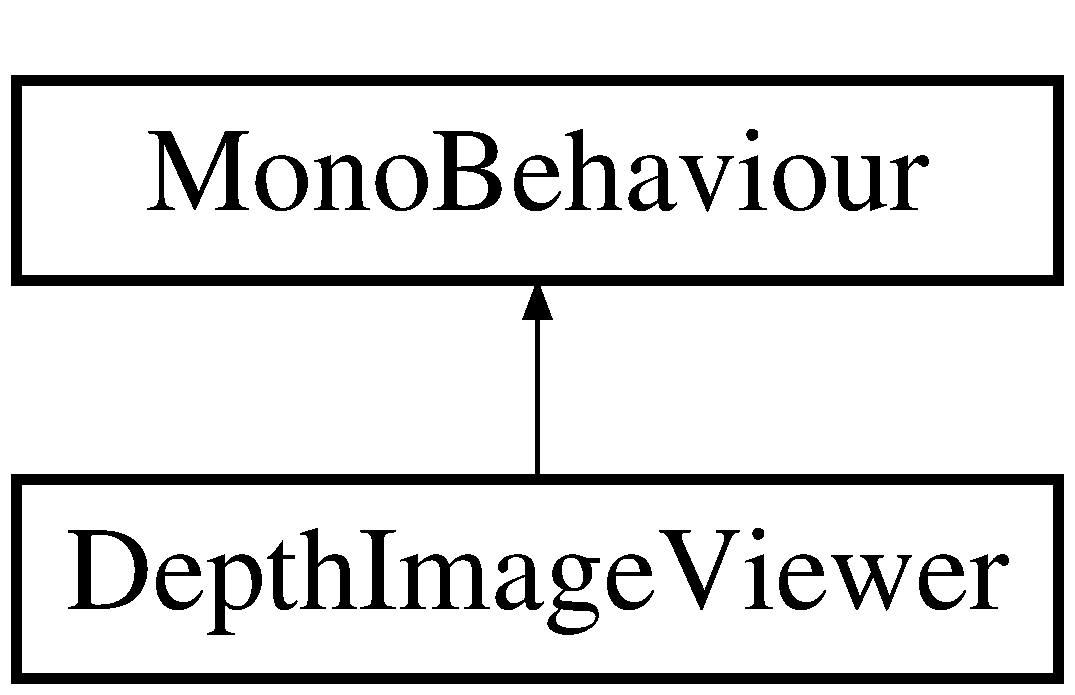
\includegraphics[height=2.000000cm]{class_depth_image_viewer}
\end{center}
\end{figure}


The documentation for this class was generated from the following file\+:\begin{DoxyCompactItemize}
\item 
Assets/\+Depth\+Collider\+Demo/\+Scripts/Depth\+Image\+Viewer.\+cs\end{DoxyCompactItemize}

\hypertarget{class_egg_mover}{}\section{Egg\+Mover Class Reference}
\label{class_egg_mover}\index{Egg\+Mover@{Egg\+Mover}}
Inheritance diagram for Egg\+Mover\+:\begin{figure}[H]
\begin{center}
\leavevmode
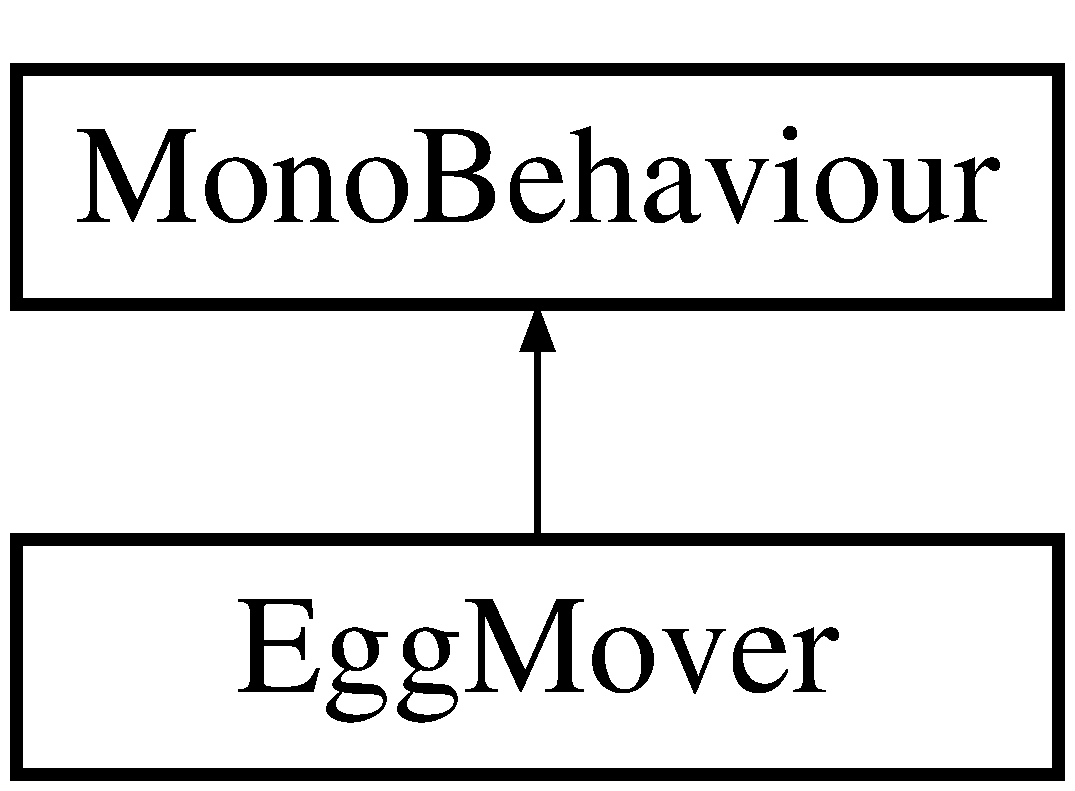
\includegraphics[height=2.000000cm]{class_egg_mover}
\end{center}
\end{figure}


The documentation for this class was generated from the following file\+:\begin{DoxyCompactItemize}
\item 
Assets/\+Depth\+Collider\+Demo/\+Scripts/Egg\+Mover.\+cs\end{DoxyCompactItemize}

\hypertarget{class_egg_spawner}{}\section{Egg\+Spawner Class Reference}
\label{class_egg_spawner}\index{Egg\+Spawner@{Egg\+Spawner}}
Inheritance diagram for Egg\+Spawner\+:\begin{figure}[H]
\begin{center}
\leavevmode
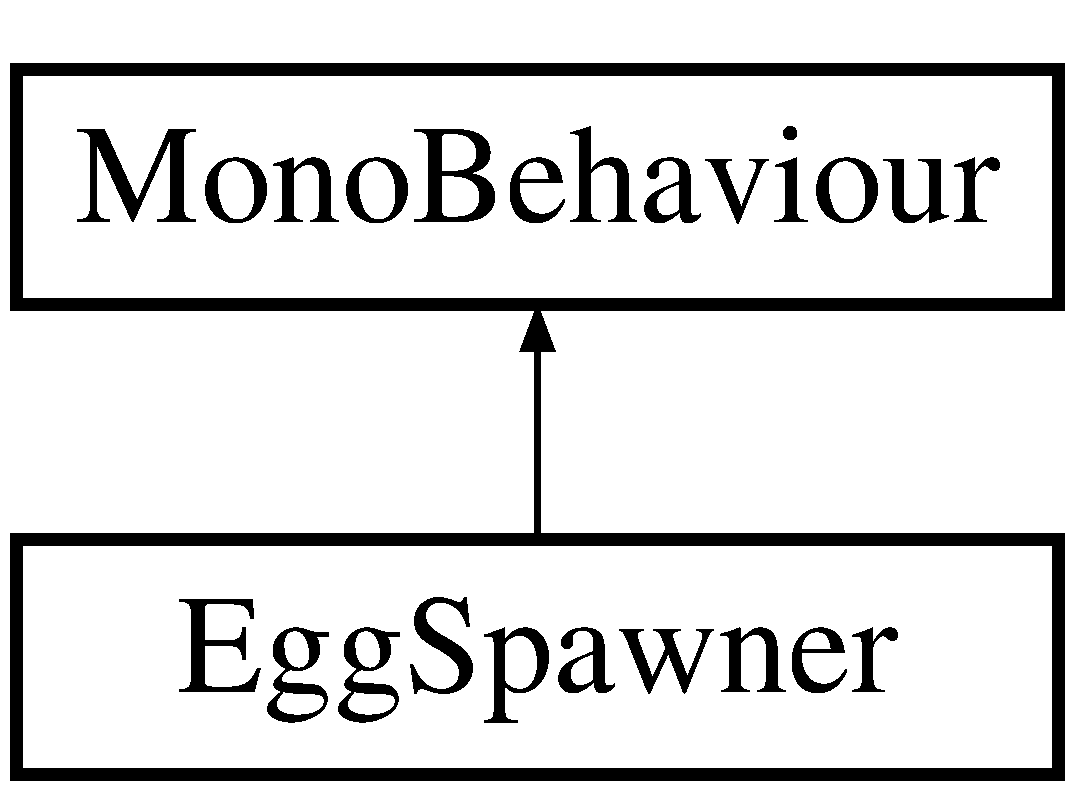
\includegraphics[height=2.000000cm]{class_egg_spawner}
\end{center}
\end{figure}
\subsection*{Public Attributes}
\begin{DoxyCompactItemize}
\item 
\mbox{\Hypertarget{class_egg_spawner_a602ae008f92d10eff823fba342fee470}\label{class_egg_spawner_a602ae008f92d10eff823fba342fee470}} 
Transform {\bfseries egg\+Prefab}
\end{DoxyCompactItemize}


The documentation for this class was generated from the following file\+:\begin{DoxyCompactItemize}
\item 
Assets/\+Depth\+Collider\+Demo/\+Scripts/Egg\+Spawner.\+cs\end{DoxyCompactItemize}

\hypertarget{class_follow_user_rotation}{}\section{Follow\+User\+Rotation Class Reference}
\label{class_follow_user_rotation}\index{Follow\+User\+Rotation@{Follow\+User\+Rotation}}
Inheritance diagram for Follow\+User\+Rotation\+:\begin{figure}[H]
\begin{center}
\leavevmode
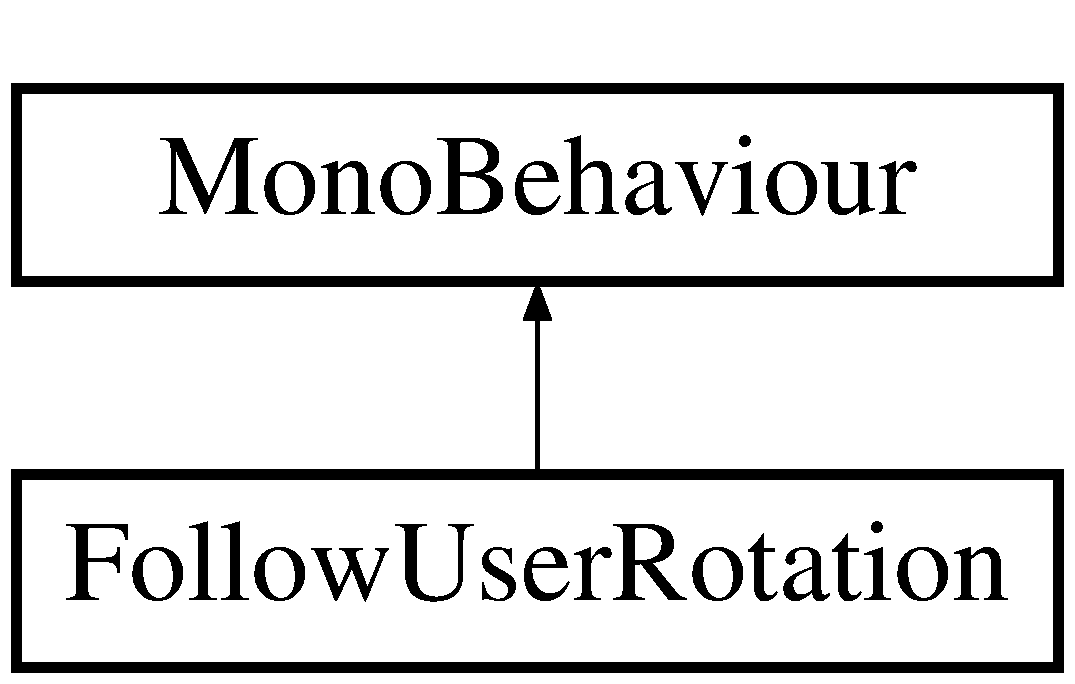
\includegraphics[height=2.000000cm]{class_follow_user_rotation}
\end{center}
\end{figure}


The documentation for this class was generated from the following file\+:\begin{DoxyCompactItemize}
\item 
Assets/\+Kinect\+Scripts/\+Samples/Follow\+User\+Rotation.\+cs\end{DoxyCompactItemize}

\hypertarget{struct_kinect_gestures_1_1_gesture_data}{}\section{Kinect\+Gestures.\+Gesture\+Data Struct Reference}
\label{struct_kinect_gestures_1_1_gesture_data}\index{Kinect\+Gestures.\+Gesture\+Data@{Kinect\+Gestures.\+Gesture\+Data}}
\subsection*{Public Attributes}
\begin{DoxyCompactItemize}
\item 
\mbox{\Hypertarget{struct_kinect_gestures_1_1_gesture_data_a2eecc1fbd066859e74b0423a01a30afe}\label{struct_kinect_gestures_1_1_gesture_data_a2eecc1fbd066859e74b0423a01a30afe}} 
uint {\bfseries user\+Id}
\item 
\mbox{\Hypertarget{struct_kinect_gestures_1_1_gesture_data_af5c52072f1be6066a9cb5aba4ea46049}\label{struct_kinect_gestures_1_1_gesture_data_af5c52072f1be6066a9cb5aba4ea46049}} 
Gestures {\bfseries gesture}
\item 
\mbox{\Hypertarget{struct_kinect_gestures_1_1_gesture_data_a7f27c5e9bb6d3cd1252d2673f7688b11}\label{struct_kinect_gestures_1_1_gesture_data_a7f27c5e9bb6d3cd1252d2673f7688b11}} 
int {\bfseries state}
\item 
\mbox{\Hypertarget{struct_kinect_gestures_1_1_gesture_data_aa00c7d789685454b062644ff2e0faab1}\label{struct_kinect_gestures_1_1_gesture_data_aa00c7d789685454b062644ff2e0faab1}} 
float {\bfseries timestamp}
\item 
\mbox{\Hypertarget{struct_kinect_gestures_1_1_gesture_data_a89196077f253100f4daf4e7011329718}\label{struct_kinect_gestures_1_1_gesture_data_a89196077f253100f4daf4e7011329718}} 
int {\bfseries joint}
\item 
\mbox{\Hypertarget{struct_kinect_gestures_1_1_gesture_data_a3ff3d29a5674237299883187d060d803}\label{struct_kinect_gestures_1_1_gesture_data_a3ff3d29a5674237299883187d060d803}} 
Vector3 {\bfseries joint\+Pos}
\item 
\mbox{\Hypertarget{struct_kinect_gestures_1_1_gesture_data_a4517d45cbb891529a2c92d66df20bdd7}\label{struct_kinect_gestures_1_1_gesture_data_a4517d45cbb891529a2c92d66df20bdd7}} 
Vector3 {\bfseries screen\+Pos}
\item 
\mbox{\Hypertarget{struct_kinect_gestures_1_1_gesture_data_a260eaec139e766705ede39c859d0e85a}\label{struct_kinect_gestures_1_1_gesture_data_a260eaec139e766705ede39c859d0e85a}} 
float {\bfseries tag\+Float}
\item 
\mbox{\Hypertarget{struct_kinect_gestures_1_1_gesture_data_a934e1ed945b1b20c731b25bc164e6926}\label{struct_kinect_gestures_1_1_gesture_data_a934e1ed945b1b20c731b25bc164e6926}} 
Vector3 {\bfseries tag\+Vector}
\item 
\mbox{\Hypertarget{struct_kinect_gestures_1_1_gesture_data_aba4db03fef47f5306304c1afbf219c19}\label{struct_kinect_gestures_1_1_gesture_data_aba4db03fef47f5306304c1afbf219c19}} 
Vector3 {\bfseries tag\+Vector2}
\item 
\mbox{\Hypertarget{struct_kinect_gestures_1_1_gesture_data_ae64ae7e44edad3e1e847d5925420e398}\label{struct_kinect_gestures_1_1_gesture_data_ae64ae7e44edad3e1e847d5925420e398}} 
float {\bfseries progress}
\item 
\mbox{\Hypertarget{struct_kinect_gestures_1_1_gesture_data_a0b074cbc71e98749d5598b704793dd0e}\label{struct_kinect_gestures_1_1_gesture_data_a0b074cbc71e98749d5598b704793dd0e}} 
bool {\bfseries complete}
\item 
\mbox{\Hypertarget{struct_kinect_gestures_1_1_gesture_data_ae0f3a74a6a3d3153777b63154eb943e1}\label{struct_kinect_gestures_1_1_gesture_data_ae0f3a74a6a3d3153777b63154eb943e1}} 
bool {\bfseries cancelled}
\item 
\mbox{\Hypertarget{struct_kinect_gestures_1_1_gesture_data_a08fa67c179b32654403e2e8a9247e290}\label{struct_kinect_gestures_1_1_gesture_data_a08fa67c179b32654403e2e8a9247e290}} 
List$<$ Gestures $>$ {\bfseries check\+For\+Gestures}
\item 
\mbox{\Hypertarget{struct_kinect_gestures_1_1_gesture_data_a108cda0a71bed75455eef681344db6c4}\label{struct_kinect_gestures_1_1_gesture_data_a108cda0a71bed75455eef681344db6c4}} 
float {\bfseries start\+Tracking\+At\+Time}
\end{DoxyCompactItemize}


The documentation for this struct was generated from the following file\+:\begin{DoxyCompactItemize}
\item 
Assets/\+Kinect\+Scripts/Kinect\+Gestures.\+cs\end{DoxyCompactItemize}

\hypertarget{class_gesture_listener}{}\section{Gesture\+Listener Class Reference}
\label{class_gesture_listener}\index{Gesture\+Listener@{Gesture\+Listener}}
Inheritance diagram for Gesture\+Listener\+:\begin{figure}[H]
\begin{center}
\leavevmode
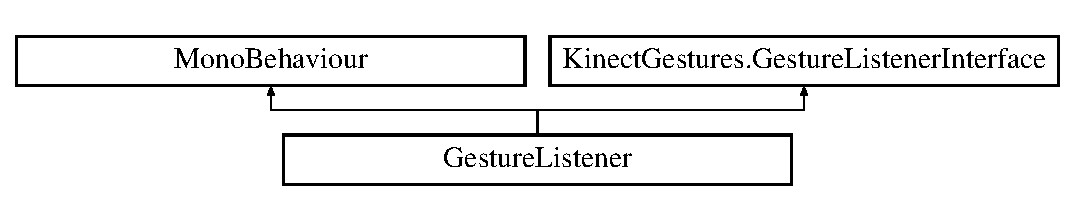
\includegraphics[height=2.000000cm]{class_gesture_listener}
\end{center}
\end{figure}
\subsection*{Public Member Functions}
\begin{DoxyCompactItemize}
\item 
\mbox{\Hypertarget{class_gesture_listener_ab6f6cda6d3d33adbbc95a958adbcd4ba}\label{class_gesture_listener_ab6f6cda6d3d33adbbc95a958adbcd4ba}} 
bool {\bfseries Is\+Swipe\+Left} ()
\item 
\mbox{\Hypertarget{class_gesture_listener_a60dca02bf253396f24afe92d4c8d3b0e}\label{class_gesture_listener_a60dca02bf253396f24afe92d4c8d3b0e}} 
bool {\bfseries Is\+Swipe\+Right} ()
\item 
\mbox{\Hypertarget{class_gesture_listener_a193b273dd51d42ff2dfb9bacb9971e2c}\label{class_gesture_listener_a193b273dd51d42ff2dfb9bacb9971e2c}} 
void {\bfseries User\+Detected} (uint user\+Id, int user\+Index)
\item 
\mbox{\Hypertarget{class_gesture_listener_aee0bc269374b5641ac71d6a0720b5309}\label{class_gesture_listener_aee0bc269374b5641ac71d6a0720b5309}} 
void {\bfseries User\+Lost} (uint user\+Id, int user\+Index)
\item 
\mbox{\Hypertarget{class_gesture_listener_a133180515cc44003a7668f7ad4b79984}\label{class_gesture_listener_a133180515cc44003a7668f7ad4b79984}} 
void {\bfseries Gesture\+In\+Progress} (uint user\+Id, int user\+Index, Kinect\+Gestures.\+Gestures gesture, float progress, Kinect\+Wrapper.\+Nui\+Skeleton\+Position\+Index joint, Vector3 screen\+Pos)
\item 
\mbox{\Hypertarget{class_gesture_listener_ac2de008d4400c5da2bc7810430bdd50c}\label{class_gesture_listener_ac2de008d4400c5da2bc7810430bdd50c}} 
bool {\bfseries Gesture\+Completed} (uint user\+Id, int user\+Index, Kinect\+Gestures.\+Gestures gesture, Kinect\+Wrapper.\+Nui\+Skeleton\+Position\+Index joint, Vector3 screen\+Pos)
\item 
\mbox{\Hypertarget{class_gesture_listener_a4c3782eff4d837d287988828b8e4970f}\label{class_gesture_listener_a4c3782eff4d837d287988828b8e4970f}} 
bool {\bfseries Gesture\+Cancelled} (uint user\+Id, int user\+Index, Kinect\+Gestures.\+Gestures gesture, Kinect\+Wrapper.\+Nui\+Skeleton\+Position\+Index joint)
\end{DoxyCompactItemize}
\subsection*{Public Attributes}
\begin{DoxyCompactItemize}
\item 
\mbox{\Hypertarget{class_gesture_listener_a86c29857f42757e33c06574f2762be0c}\label{class_gesture_listener_a86c29857f42757e33c06574f2762be0c}} 
G\+U\+I\+Text {\bfseries Gesture\+Info}
\end{DoxyCompactItemize}


The documentation for this class was generated from the following file\+:\begin{DoxyCompactItemize}
\item 
Assets/\+Gestures\+Demo/\+Scripts/Gesture\+Listener.\+cs\end{DoxyCompactItemize}

\hypertarget{interface_kinect_gestures_1_1_gesture_listener_interface}{}\section{Kinect\+Gestures.\+Gesture\+Listener\+Interface Interface Reference}
\label{interface_kinect_gestures_1_1_gesture_listener_interface}\index{Kinect\+Gestures.\+Gesture\+Listener\+Interface@{Kinect\+Gestures.\+Gesture\+Listener\+Interface}}
Inheritance diagram for Kinect\+Gestures.\+Gesture\+Listener\+Interface\+:\begin{figure}[H]
\begin{center}
\leavevmode
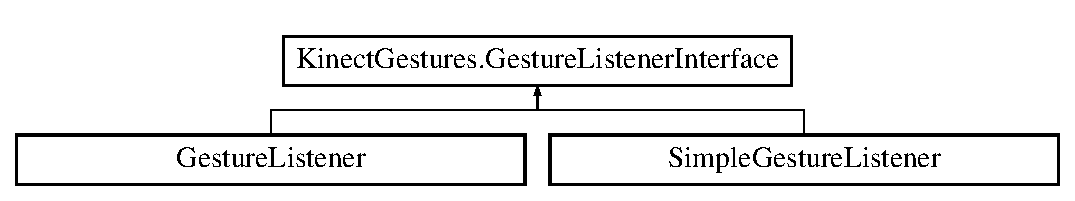
\includegraphics[height=2.000000cm]{interface_kinect_gestures_1_1_gesture_listener_interface}
\end{center}
\end{figure}
\subsection*{Public Member Functions}
\begin{DoxyCompactItemize}
\item 
\mbox{\Hypertarget{interface_kinect_gestures_1_1_gesture_listener_interface_a7d5f8a883f6ceceac7c66349eb2dd254}\label{interface_kinect_gestures_1_1_gesture_listener_interface_a7d5f8a883f6ceceac7c66349eb2dd254}} 
void {\bfseries User\+Detected} (uint user\+Id, int user\+Index)
\item 
\mbox{\Hypertarget{interface_kinect_gestures_1_1_gesture_listener_interface_a6efb826325af8b69ea7523e44d0d199e}\label{interface_kinect_gestures_1_1_gesture_listener_interface_a6efb826325af8b69ea7523e44d0d199e}} 
void {\bfseries User\+Lost} (uint user\+Id, int user\+Index)
\item 
\mbox{\Hypertarget{interface_kinect_gestures_1_1_gesture_listener_interface_a9dde26ecbcbf4d8da10e36adc4005fc4}\label{interface_kinect_gestures_1_1_gesture_listener_interface_a9dde26ecbcbf4d8da10e36adc4005fc4}} 
void {\bfseries Gesture\+In\+Progress} (uint user\+Id, int user\+Index, Gestures gesture, float progress, Kinect\+Wrapper.\+Nui\+Skeleton\+Position\+Index joint, Vector3 screen\+Pos)
\item 
\mbox{\Hypertarget{interface_kinect_gestures_1_1_gesture_listener_interface_a469fe8287f4b19f061568a0ec0425df9}\label{interface_kinect_gestures_1_1_gesture_listener_interface_a469fe8287f4b19f061568a0ec0425df9}} 
bool {\bfseries Gesture\+Completed} (uint user\+Id, int user\+Index, Gestures gesture, Kinect\+Wrapper.\+Nui\+Skeleton\+Position\+Index joint, Vector3 screen\+Pos)
\item 
\mbox{\Hypertarget{interface_kinect_gestures_1_1_gesture_listener_interface_ab0cfad45796c5974c4bc3464689b0387}\label{interface_kinect_gestures_1_1_gesture_listener_interface_ab0cfad45796c5974c4bc3464689b0387}} 
bool {\bfseries Gesture\+Cancelled} (uint user\+Id, int user\+Index, Gestures gesture, Kinect\+Wrapper.\+Nui\+Skeleton\+Position\+Index joint)
\end{DoxyCompactItemize}


The documentation for this interface was generated from the following file\+:\begin{DoxyCompactItemize}
\item 
Assets/\+Kinect\+Scripts/Kinect\+Gestures.\+cs\end{DoxyCompactItemize}

\hypertarget{class_get_joint_position_demo}{}\section{Get\+Joint\+Position\+Demo Class Reference}
\label{class_get_joint_position_demo}\index{Get\+Joint\+Position\+Demo@{Get\+Joint\+Position\+Demo}}
Inheritance diagram for Get\+Joint\+Position\+Demo\+:\begin{figure}[H]
\begin{center}
\leavevmode
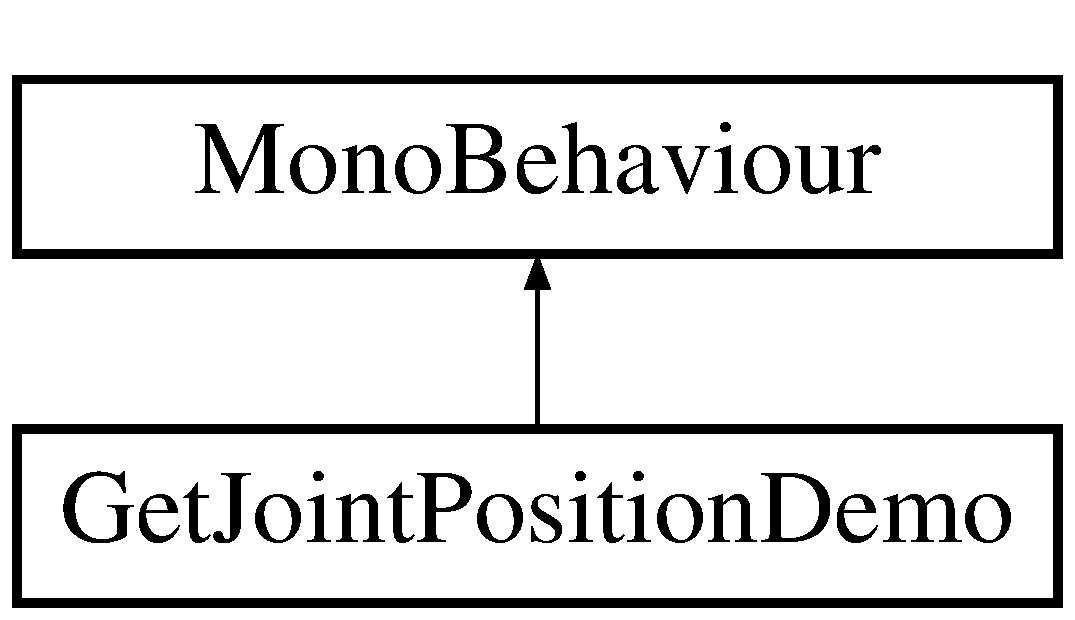
\includegraphics[height=2.000000cm]{class_get_joint_position_demo}
\end{center}
\end{figure}
\subsection*{Public Attributes}
\begin{DoxyCompactItemize}
\item 
\mbox{\Hypertarget{class_get_joint_position_demo_a2f1433fb9f5277878a276beee5d9c44b}\label{class_get_joint_position_demo_a2f1433fb9f5277878a276beee5d9c44b}} 
Kinect\+Wrapper.\+Nui\+Skeleton\+Position\+Index {\bfseries joint} = Kinect\+Wrapper.\+Nui\+Skeleton\+Position\+Index.\+Hand\+Right
\item 
\mbox{\Hypertarget{class_get_joint_position_demo_aed3f43661ae874b501e952946525ede7}\label{class_get_joint_position_demo_aed3f43661ae874b501e952946525ede7}} 
Vector3 {\bfseries output\+Position}
\item 
\mbox{\Hypertarget{class_get_joint_position_demo_a410f993a82c4a0efa8264feec6ec4dde}\label{class_get_joint_position_demo_a410f993a82c4a0efa8264feec6ec4dde}} 
bool {\bfseries is\+Saving} = false
\item 
\mbox{\Hypertarget{class_get_joint_position_demo_a17dea2adb7bf2ba7f7ac9ba017f9a4a4}\label{class_get_joint_position_demo_a17dea2adb7bf2ba7f7ac9ba017f9a4a4}} 
float {\bfseries seconds\+To\+Save} = 0f
\item 
\mbox{\Hypertarget{class_get_joint_position_demo_a6ad9df96efa58c4bd47775606df9cf68}\label{class_get_joint_position_demo_a6ad9df96efa58c4bd47775606df9cf68}} 
string {\bfseries save\+File\+Path} = \char`\"{}joint\+\_\+pos.\+csv\char`\"{}
\end{DoxyCompactItemize}


The documentation for this class was generated from the following file\+:\begin{DoxyCompactItemize}
\item 
Assets/\+Kinect\+Scripts/\+Samples/Get\+Joint\+Position\+Demo.\+cs\end{DoxyCompactItemize}

\hypertarget{interface_kinect_wrapper_1_1_i_nui_frame_texture}{}\section{Kinect\+Wrapper.\+I\+Nui\+Frame\+Texture Interface Reference}
\label{interface_kinect_wrapper_1_1_i_nui_frame_texture}\index{Kinect\+Wrapper.\+I\+Nui\+Frame\+Texture@{Kinect\+Wrapper.\+I\+Nui\+Frame\+Texture}}
\subsection*{Public Member Functions}
\begin{DoxyCompactItemize}
\item 
\mbox{\Hypertarget{interface_kinect_wrapper_1_1_i_nui_frame_texture_ab8209a380175eb9615897d3bfaaf4814}\label{interface_kinect_wrapper_1_1_i_nui_frame_texture_ab8209a380175eb9615897d3bfaaf4814}} 
int {\bfseries Buffer\+Len} ()
\item 
\mbox{\Hypertarget{interface_kinect_wrapper_1_1_i_nui_frame_texture_a26276f514de9e0deb6230593892d594d}\label{interface_kinect_wrapper_1_1_i_nui_frame_texture_a26276f514de9e0deb6230593892d594d}} 
int {\bfseries Pitch} ()
\item 
\mbox{\Hypertarget{interface_kinect_wrapper_1_1_i_nui_frame_texture_a220d82f521ec76fc83403c324c7cb797}\label{interface_kinect_wrapper_1_1_i_nui_frame_texture_a220d82f521ec76fc83403c324c7cb797}} 
int {\bfseries Lock\+Rect} (uint Level, ref \mbox{\hyperlink{struct_kinect_wrapper_1_1_nui_locked_rect}{Nui\+Locked\+Rect}} p\+Locked\+Rect, Int\+Ptr p\+Rect, uint Flags)
\item 
\mbox{\Hypertarget{interface_kinect_wrapper_1_1_i_nui_frame_texture_a852f650aae40e55958a4780017e3c191}\label{interface_kinect_wrapper_1_1_i_nui_frame_texture_a852f650aae40e55958a4780017e3c191}} 
int {\bfseries Get\+Level\+Desc} (uint Level, ref \mbox{\hyperlink{struct_kinect_wrapper_1_1_nui_surface_desc}{Nui\+Surface\+Desc}} p\+Desc)
\item 
\mbox{\Hypertarget{interface_kinect_wrapper_1_1_i_nui_frame_texture_a51d2dd6849585641662053fc5f2ec36f}\label{interface_kinect_wrapper_1_1_i_nui_frame_texture_a51d2dd6849585641662053fc5f2ec36f}} 
int {\bfseries Unlock\+Rect} (uint Level)
\end{DoxyCompactItemize}


The documentation for this interface was generated from the following file\+:\begin{DoxyCompactItemize}
\item 
Assets/\+Kinect\+Scripts/Kinect\+Wrapper.\+cs\end{DoxyCompactItemize}

\hypertarget{class_joint_positions_filter}{}\section{Joint\+Positions\+Filter Class Reference}
\label{class_joint_positions_filter}\index{Joint\+Positions\+Filter@{Joint\+Positions\+Filter}}


Implementation of a Holt Double Exponential Smoothing filter. The double exponential smooths the curve and predicts. There is also noise jitter removal. And maximum prediction bounds. The parameters are commented in the Init function.  


\subsection*{Public Member Functions}
\begin{DoxyCompactItemize}
\item 
\mbox{\Hypertarget{class_joint_positions_filter_aab7201ee120c14aec70402cc6a7ac1f9}\label{class_joint_positions_filter_aab7201ee120c14aec70402cc6a7ac1f9}} 
\mbox{\hyperlink{class_joint_positions_filter_aab7201ee120c14aec70402cc6a7ac1f9}{Joint\+Positions\+Filter}} ()
\begin{DoxyCompactList}\small\item\em Initializes a new instance of the class. \end{DoxyCompactList}\item 
\mbox{\Hypertarget{class_joint_positions_filter_a15e0a5e5df56f73100e78bc7f9b9274e}\label{class_joint_positions_filter_a15e0a5e5df56f73100e78bc7f9b9274e}} 
void {\bfseries Init} ()
\item 
void \mbox{\hyperlink{class_joint_positions_filter_a3815ebb632cddd00240f03a8ba0b429a}{Init}} (float smoothing\+Value, float correction\+Value, float prediction\+Value, float jitter\+Radius\+Value, float max\+Deviation\+Radius\+Value)
\begin{DoxyCompactList}\small\item\em Initialize the filter with a set of manually specified Transform\+Smooth\+Parameters. \end{DoxyCompactList}\item 
\mbox{\Hypertarget{class_joint_positions_filter_a5ed2fce9405fbd1231bfb184400a448e}\label{class_joint_positions_filter_a5ed2fce9405fbd1231bfb184400a448e}} 
void {\bfseries Init} (\mbox{\hyperlink{struct_kinect_wrapper_1_1_nui_transform_smooth_parameters}{Kinect\+Wrapper.\+Nui\+Transform\+Smooth\+Parameters}} smoothing\+Parameters)
\item 
\mbox{\Hypertarget{class_joint_positions_filter_a25feb954527213cd0b28d803001f29ce}\label{class_joint_positions_filter_a25feb954527213cd0b28d803001f29ce}} 
void {\bfseries Reset} ()
\item 
\mbox{\Hypertarget{class_joint_positions_filter_abdef3ba9b7efe903f10c4ba628e674ed}\label{class_joint_positions_filter_abdef3ba9b7efe903f10c4ba628e674ed}} 
void {\bfseries Update\+Filter} (ref \mbox{\hyperlink{struct_kinect_wrapper_1_1_nui_skeleton_data}{Kinect\+Wrapper.\+Nui\+Skeleton\+Data}} skeleton)
\end{DoxyCompactItemize}
\subsection*{Protected Member Functions}
\begin{DoxyCompactItemize}
\item 
\mbox{\Hypertarget{class_joint_positions_filter_a8dcf8fb2da8cfcb5f76599df193f00d5}\label{class_joint_positions_filter_a8dcf8fb2da8cfcb5f76599df193f00d5}} 
void {\bfseries Filter\+Joint} (ref \mbox{\hyperlink{struct_kinect_wrapper_1_1_nui_skeleton_data}{Kinect\+Wrapper.\+Nui\+Skeleton\+Data}} skeleton, int joint\+Index, ref \mbox{\hyperlink{struct_kinect_wrapper_1_1_nui_transform_smooth_parameters}{Kinect\+Wrapper.\+Nui\+Transform\+Smooth\+Parameters}} smoothing\+Parameters)
\end{DoxyCompactItemize}


\subsection{Detailed Description}
Implementation of a Holt Double Exponential Smoothing filter. The double exponential smooths the curve and predicts. There is also noise jitter removal. And maximum prediction bounds. The parameters are commented in the Init function. 



\subsection{Member Function Documentation}
\mbox{\Hypertarget{class_joint_positions_filter_a3815ebb632cddd00240f03a8ba0b429a}\label{class_joint_positions_filter_a3815ebb632cddd00240f03a8ba0b429a}} 
\index{Joint\+Positions\+Filter@{Joint\+Positions\+Filter}!Init@{Init}}
\index{Init@{Init}!Joint\+Positions\+Filter@{Joint\+Positions\+Filter}}
\subsubsection{\texorpdfstring{Init()}{Init()}}
{\footnotesize\ttfamily void Joint\+Positions\+Filter.\+Init (\begin{DoxyParamCaption}\item[{float}]{smoothing\+Value,  }\item[{float}]{correction\+Value,  }\item[{float}]{prediction\+Value,  }\item[{float}]{jitter\+Radius\+Value,  }\item[{float}]{max\+Deviation\+Radius\+Value }\end{DoxyParamCaption})}



Initialize the filter with a set of manually specified Transform\+Smooth\+Parameters. 


\begin{DoxyParams}{Parameters}
{\em smoothing\+Value} & Smoothing = \mbox{[}0..1\mbox{]}, lower values is closer to the raw data and more noisy.\\
\hline
{\em correction\+Value} & Correction = \mbox{[}0..1\mbox{]}, higher values correct faster and feel more responsive.\\
\hline
{\em prediction\+Value} & Prediction = \mbox{[}0..n\mbox{]}, how many frames into the future we want to predict.\\
\hline
{\em jitter\+Radius\+Value} & Jitter\+Radius = The deviation distance in m that defines jitter.\\
\hline
{\em max\+Deviation\+Radius\+Value} & Max\+Deviation = The maximum distance in m that filtered positions are allowed to deviate from raw data.\\
\hline
\end{DoxyParams}


The documentation for this class was generated from the following file\+:\begin{DoxyCompactItemize}
\item 
Assets/\+Kinect\+Scripts/\+Filters/Joint\+Positions\+Filter.\+cs\end{DoxyCompactItemize}

\hypertarget{class_kinect_gestures}{}\section{Kinect\+Gestures Class Reference}
\label{class_kinect_gestures}\index{Kinect\+Gestures@{Kinect\+Gestures}}
\subsection*{Classes}
\begin{DoxyCompactItemize}
\item 
struct \mbox{\hyperlink{struct_kinect_gestures_1_1_gesture_data}{Gesture\+Data}}
\item 
interface \mbox{\hyperlink{interface_kinect_gestures_1_1_gesture_listener_interface}{Gesture\+Listener\+Interface}}
\end{DoxyCompactItemize}
\subsection*{Public Types}
\begin{DoxyCompactItemize}
\item 
\mbox{\Hypertarget{class_kinect_gestures_ae979f8f37dd7730c916cd84d7894a652}\label{class_kinect_gestures_ae979f8f37dd7730c916cd84d7894a652}} 
enum {\bfseries Gestures} \{ \newline
{\bfseries None} = 0, 
{\bfseries Raise\+Right\+Hand}, 
{\bfseries Raise\+Left\+Hand}, 
{\bfseries Psi}, 
\newline
{\bfseries Tpose}, 
{\bfseries Stop}, 
{\bfseries Wave}, 
{\bfseries Click}, 
\newline
{\bfseries Swipe\+Left}, 
{\bfseries Swipe\+Right}, 
{\bfseries Swipe\+Up}, 
{\bfseries Swipe\+Down}, 
\newline
{\bfseries Right\+Hand\+Cursor}, 
{\bfseries Left\+Hand\+Cursor}, 
{\bfseries Zoom\+Out}, 
{\bfseries Zoom\+In}, 
\newline
{\bfseries Wheel}, 
{\bfseries Jump}, 
{\bfseries Squat}, 
{\bfseries Push}, 
\newline
{\bfseries Pull}
 \}
\end{DoxyCompactItemize}
\subsection*{Static Public Member Functions}
\begin{DoxyCompactItemize}
\item 
\mbox{\Hypertarget{class_kinect_gestures_a4e572c3f5b759588e2af549ff90e63c4}\label{class_kinect_gestures_a4e572c3f5b759588e2af549ff90e63c4}} 
static void {\bfseries Check\+For\+Gesture} (uint user\+Id, ref \mbox{\hyperlink{struct_kinect_gestures_1_1_gesture_data}{Gesture\+Data}} gesture\+Data, float timestamp, ref Vector3\mbox{[}$\,$\mbox{]} joints\+Pos, ref bool\mbox{[}$\,$\mbox{]} joints\+Tracked)
\end{DoxyCompactItemize}


The documentation for this class was generated from the following file\+:\begin{DoxyCompactItemize}
\item 
Assets/\+Kinect\+Scripts/Kinect\+Gestures.\+cs\end{DoxyCompactItemize}

\hypertarget{class_kinect_helper}{}\section{Kinect\+Helper Class Reference}
\label{class_kinect_helper}\index{Kinect\+Helper@{Kinect\+Helper}}
\subsection*{Static Public Member Functions}
\begin{DoxyCompactItemize}
\item 
\mbox{\Hypertarget{class_kinect_helper_a9363f32b91490038a17f0d976c179cab}\label{class_kinect_helper_a9363f32b91490038a17f0d976c179cab}} 
static bool {\bfseries Joint\+Position\+Is\+Valid} (Vector3 joint\+Position)
\item 
\mbox{\Hypertarget{class_kinect_helper_ad32dda60dab4b3ca51dab2ff87c23ca4}\label{class_kinect_helper_ad32dda60dab4b3ca51dab2ff87c23ca4}} 
static bool {\bfseries Bone\+Orientation\+Is\+Valid} (Quaternion bone\+Orientation)
\item 
\mbox{\Hypertarget{class_kinect_helper_a329affc063588a2df0f41c31f8b0435a}\label{class_kinect_helper_a329affc063588a2df0f41c31f8b0435a}} 
static bool {\bfseries Is\+Tracked} (\mbox{\hyperlink{struct_kinect_wrapper_1_1_nui_skeleton_data}{Kinect\+Wrapper.\+Nui\+Skeleton\+Data}} skeleton, int joint\+Index)
\item 
\mbox{\Hypertarget{class_kinect_helper_abcce6f17357f234fd21fdb167aed3f2b}\label{class_kinect_helper_abcce6f17357f234fd21fdb167aed3f2b}} 
static bool {\bfseries Is\+Tracked\+Or\+Inferred} (\mbox{\hyperlink{struct_kinect_wrapper_1_1_nui_skeleton_data}{Kinect\+Wrapper.\+Nui\+Skeleton\+Data}} skeleton, int joint\+Index)
\item 
\mbox{\Hypertarget{class_kinect_helper_a7cf4d92f0f65a88d27aa2a821b647d83}\label{class_kinect_helper_a7cf4d92f0f65a88d27aa2a821b647d83}} 
static Quaternion {\bfseries Rotation\+Between\+Quaternions} (Quaternion quaternionA, Quaternion quaternionB)
\item 
\mbox{\Hypertarget{class_kinect_helper_a3b96bc4fca262eff905577cee615280e}\label{class_kinect_helper_a3b96bc4fca262eff905577cee615280e}} 
static Quaternion {\bfseries Enhanced\+Quaternion\+Slerp} (Quaternion quaternionA, Quaternion quaternionB, float amount)
\item 
\mbox{\Hypertarget{class_kinect_helper_a82e8bb56dfa8c75fa5d2e77fe1930fd9}\label{class_kinect_helper_a82e8bb56dfa8c75fa5d2e77fe1930fd9}} 
static Quaternion {\bfseries Ensure\+Quaternion\+Neighborhood} (Quaternion quaternionA, Quaternion quaternionB)
\item 
\mbox{\Hypertarget{class_kinect_helper_a3a634ac394a018cc8207634bf74e751e}\label{class_kinect_helper_a3a634ac394a018cc8207634bf74e751e}} 
static float {\bfseries Quaternion\+Angle} (Quaternion rotation)
\item 
\mbox{\Hypertarget{class_kinect_helper_aa5094dc4f70d1f067e23aaefa2280d5e}\label{class_kinect_helper_aa5094dc4f70d1f067e23aaefa2280d5e}} 
static void {\bfseries Lerp\+And\+Apply} (ref \mbox{\hyperlink{struct_kinect_wrapper_1_1_nui_skeleton_data}{Kinect\+Wrapper.\+Nui\+Skeleton\+Data}} skeleton, int joint\+Index, Vector3 new\+Joint\+Pos, float lerp\+Value, Kinect\+Wrapper.\+Nui\+Skeleton\+Position\+Tracking\+State final\+Tracking\+State)
\item 
\mbox{\Hypertarget{class_kinect_helper_a7c8b3dbeef069ec1f12f15d939598f59}\label{class_kinect_helper_a7c8b3dbeef069ec1f12f15d939598f59}} 
static void {\bfseries Copy\+Skeleton} (ref \mbox{\hyperlink{struct_kinect_wrapper_1_1_nui_skeleton_data}{Kinect\+Wrapper.\+Nui\+Skeleton\+Data}} source, ref \mbox{\hyperlink{struct_kinect_wrapper_1_1_nui_skeleton_data}{Kinect\+Wrapper.\+Nui\+Skeleton\+Data}} destination)
\item 
\mbox{\Hypertarget{class_kinect_helper_adbd205f1683d864d65067ab28e6f33b9}\label{class_kinect_helper_adbd205f1683d864d65067ab28e6f33b9}} 
static Vector3 \mbox{\hyperlink{class_kinect_helper_adbd205f1683d864d65067ab28e6f33b9}{Vector\+Between}} (ref \mbox{\hyperlink{struct_kinect_wrapper_1_1_nui_skeleton_data}{Kinect\+Wrapper.\+Nui\+Skeleton\+Data}} skeleton, int start\+Joint, int end\+Joint)
\begin{DoxyCompactList}\small\item\em Vector\+Between calculates the Vector3 from start to end == subtract start from end. \end{DoxyCompactList}\item 
\mbox{\Hypertarget{class_kinect_helper_a188d510eee3dd71b003ccdc95b308182}\label{class_kinect_helper_a188d510eee3dd71b003ccdc95b308182}} 
static Vector4 {\bfseries Distance\+To\+Line\+Segment} (Vector3 line\+Point0, Vector3 line\+Point1, Vector3 point)
\end{DoxyCompactItemize}


The documentation for this class was generated from the following file\+:\begin{DoxyCompactItemize}
\item 
Assets/\+Kinect\+Scripts/\+Filters/Kinect\+Helper.\+cs\end{DoxyCompactItemize}

\hypertarget{class_kinect_manager}{}\section{Kinect\+Manager Class Reference}
\label{class_kinect_manager}\index{Kinect\+Manager@{Kinect\+Manager}}
Inheritance diagram for Kinect\+Manager\+:\begin{figure}[H]
\begin{center}
\leavevmode
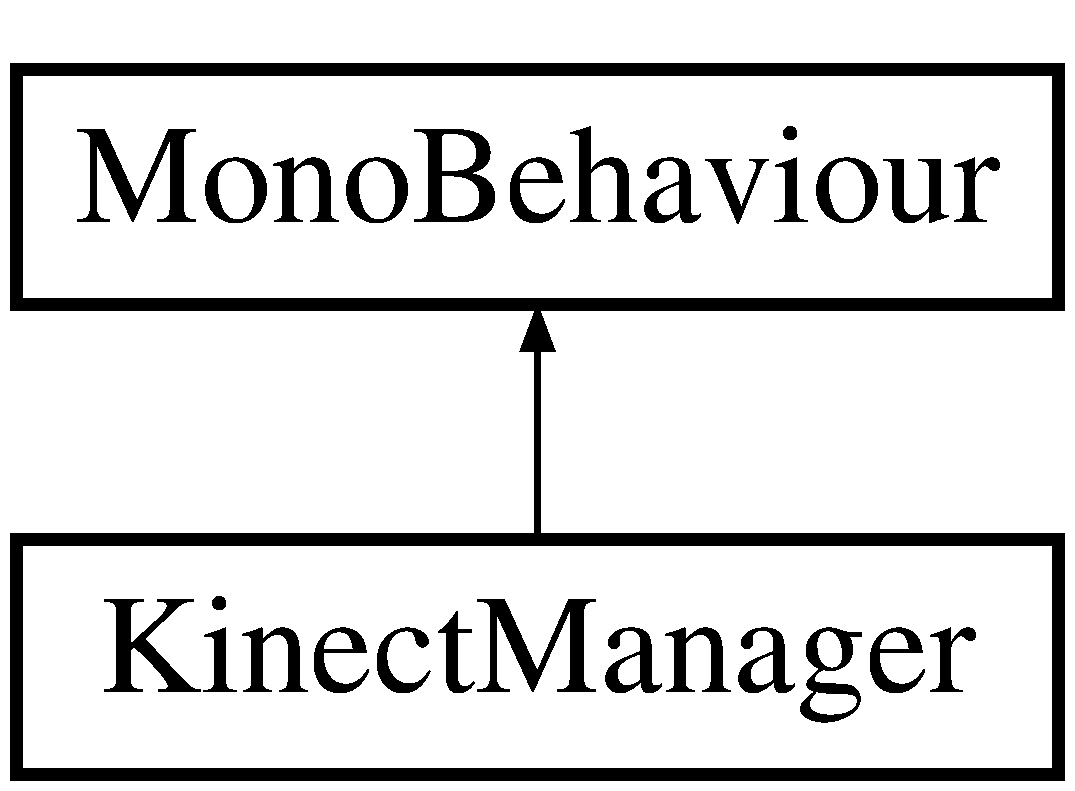
\includegraphics[height=2.000000cm]{class_kinect_manager}
\end{center}
\end{figure}
\subsection*{Public Types}
\begin{DoxyCompactItemize}
\item 
\mbox{\Hypertarget{class_kinect_manager_aec17a057770162214385062b140fe969}\label{class_kinect_manager_aec17a057770162214385062b140fe969}} 
enum {\bfseries Smoothing} \+: int \{ {\bfseries None}, 
{\bfseries Default}, 
{\bfseries Medium}, 
{\bfseries Aggressive}
 \}
\end{DoxyCompactItemize}
\subsection*{Public Member Functions}
\begin{DoxyCompactItemize}
\item 
\mbox{\Hypertarget{class_kinect_manager_aa07e9cb88230c121afccf01a22716673}\label{class_kinect_manager_aa07e9cb88230c121afccf01a22716673}} 
bool {\bfseries Is\+Initialized} ()
\item 
\mbox{\Hypertarget{class_kinect_manager_ab05138e9b95ebb46853c2c268c6f8f93}\label{class_kinect_manager_ab05138e9b95ebb46853c2c268c6f8f93}} 
ushort \mbox{[}$\,$\mbox{]} {\bfseries Get\+Raw\+Depth\+Map} ()
\item 
\mbox{\Hypertarget{class_kinect_manager_a4d82afa0b4034d9138038ed8c073ebc1}\label{class_kinect_manager_a4d82afa0b4034d9138038ed8c073ebc1}} 
ushort {\bfseries Get\+Depth\+For\+Pixel} (int x, int y)
\item 
\mbox{\Hypertarget{class_kinect_manager_aabf3116ff588a1b7ff564f54c9d93964}\label{class_kinect_manager_aabf3116ff588a1b7ff564f54c9d93964}} 
Vector2 {\bfseries Get\+Depth\+Map\+Pos\+For\+Joint\+Pos} (Vector3 pos\+Joint)
\item 
\mbox{\Hypertarget{class_kinect_manager_a66c9e59129890772e71357820026470f}\label{class_kinect_manager_a66c9e59129890772e71357820026470f}} 
Vector2 {\bfseries Get\+Color\+Map\+Pos\+For\+Depth\+Pos} (Vector2 pos\+Depth)
\item 
\mbox{\Hypertarget{class_kinect_manager_a496b20df4657e69c701e5822b12ef763}\label{class_kinect_manager_a496b20df4657e69c701e5822b12ef763}} 
Texture2D {\bfseries Get\+Users\+Lbl\+Tex} ()
\item 
\mbox{\Hypertarget{class_kinect_manager_a8b96d9349b9c0a3533057c36b6cd85d2}\label{class_kinect_manager_a8b96d9349b9c0a3533057c36b6cd85d2}} 
Texture2D {\bfseries Get\+Users\+Clr\+Tex} ()
\item 
\mbox{\Hypertarget{class_kinect_manager_a552c99f810205b173741f9898edb62bf}\label{class_kinect_manager_a552c99f810205b173741f9898edb62bf}} 
bool {\bfseries Is\+User\+Detected} ()
\item 
\mbox{\Hypertarget{class_kinect_manager_a2aa6087c65ebd098da4e0b09c4ab915e}\label{class_kinect_manager_a2aa6087c65ebd098da4e0b09c4ab915e}} 
uint {\bfseries Get\+Player1\+ID} ()
\item 
\mbox{\Hypertarget{class_kinect_manager_ac64453e53112fb39afe7b50c16c6f3ce}\label{class_kinect_manager_ac64453e53112fb39afe7b50c16c6f3ce}} 
uint {\bfseries Get\+Player2\+ID} ()
\item 
\mbox{\Hypertarget{class_kinect_manager_ac1073faa906fd0fa1974d0d064a710f8}\label{class_kinect_manager_ac1073faa906fd0fa1974d0d064a710f8}} 
int {\bfseries Get\+Player1\+Index} ()
\item 
\mbox{\Hypertarget{class_kinect_manager_a85ab5d1f3a4bf3b208291127941378a2}\label{class_kinect_manager_a85ab5d1f3a4bf3b208291127941378a2}} 
int {\bfseries Get\+Player2\+Index} ()
\item 
\mbox{\Hypertarget{class_kinect_manager_ac63bc71be34ca7399ff1a097abe9f679}\label{class_kinect_manager_ac63bc71be34ca7399ff1a097abe9f679}} 
bool {\bfseries Is\+Player\+Calibrated} (uint User\+Id)
\item 
\mbox{\Hypertarget{class_kinect_manager_a425f59c9b84e1e89f93b8b1091b4d473}\label{class_kinect_manager_a425f59c9b84e1e89f93b8b1091b4d473}} 
Vector3 {\bfseries Get\+Raw\+Skeleton\+Joint\+Pos} (uint User\+Id, int joint)
\item 
\mbox{\Hypertarget{class_kinect_manager_aca20e9d8cd5ebb481673fcf63b6b18fc}\label{class_kinect_manager_aca20e9d8cd5ebb481673fcf63b6b18fc}} 
Vector3 {\bfseries Get\+User\+Position} (uint User\+Id)
\item 
\mbox{\Hypertarget{class_kinect_manager_a7f15cd908891e9cee89520cb63f45577}\label{class_kinect_manager_a7f15cd908891e9cee89520cb63f45577}} 
Quaternion {\bfseries Get\+User\+Orientation} (uint User\+Id, bool flip)
\item 
\mbox{\Hypertarget{class_kinect_manager_ac55fb953a35d5290e0004fb9ac4cc139}\label{class_kinect_manager_ac55fb953a35d5290e0004fb9ac4cc139}} 
bool {\bfseries Is\+Joint\+Tracked} (uint User\+Id, int joint)
\item 
\mbox{\Hypertarget{class_kinect_manager_acda02655d464aaa83c8b71ca492805d3}\label{class_kinect_manager_acda02655d464aaa83c8b71ca492805d3}} 
Vector3 {\bfseries Get\+Joint\+Position} (uint User\+Id, int joint)
\item 
\mbox{\Hypertarget{class_kinect_manager_a1b74d41febb7bf73681c4a8f2f5b0f19}\label{class_kinect_manager_a1b74d41febb7bf73681c4a8f2f5b0f19}} 
Vector3 {\bfseries Get\+Joint\+Local\+Position} (uint User\+Id, int joint)
\item 
\mbox{\Hypertarget{class_kinect_manager_aa11213684be7e8f0f79ada8fb1fee9c5}\label{class_kinect_manager_aa11213684be7e8f0f79ada8fb1fee9c5}} 
Quaternion {\bfseries Get\+Joint\+Orientation} (uint User\+Id, int joint, bool flip)
\item 
\mbox{\Hypertarget{class_kinect_manager_a11b8288ad51dc8f11c05c92efb041572}\label{class_kinect_manager_a11b8288ad51dc8f11c05c92efb041572}} 
Quaternion {\bfseries Get\+Joint\+Local\+Orientation} (uint User\+Id, int joint, bool flip)
\item 
\mbox{\Hypertarget{class_kinect_manager_a5aaa167f101f8143c309300c6d8a0a21}\label{class_kinect_manager_a5aaa167f101f8143c309300c6d8a0a21}} 
Vector3 {\bfseries Get\+Direction\+Between\+Joints} (uint User\+Id, int base\+Joint, int next\+Joint, bool flipX, bool flipZ)
\item 
\mbox{\Hypertarget{class_kinect_manager_aaa496d55486a07be1bd33ab29c4aeb31}\label{class_kinect_manager_aaa496d55486a07be1bd33ab29c4aeb31}} 
void {\bfseries Detect\+Gesture} (uint User\+Id, Kinect\+Gestures.\+Gestures gesture)
\item 
\mbox{\Hypertarget{class_kinect_manager_afc3ee5ab5f438c6b89b303cdfcd7c0ae}\label{class_kinect_manager_afc3ee5ab5f438c6b89b303cdfcd7c0ae}} 
bool {\bfseries Reset\+Gesture} (uint User\+Id, Kinect\+Gestures.\+Gestures gesture)
\item 
\mbox{\Hypertarget{class_kinect_manager_afdc90787281b1b722a7369ccd82d219c}\label{class_kinect_manager_afdc90787281b1b722a7369ccd82d219c}} 
void {\bfseries Reset\+Player\+Gestures} (uint User\+Id)
\item 
\mbox{\Hypertarget{class_kinect_manager_a2ddd469d4fd9700e45561dc6a9d38f95}\label{class_kinect_manager_a2ddd469d4fd9700e45561dc6a9d38f95}} 
bool {\bfseries Delete\+Gesture} (uint User\+Id, Kinect\+Gestures.\+Gestures gesture)
\item 
\mbox{\Hypertarget{class_kinect_manager_abc1de536fb4facd54a3dc1f5b5cad2c0}\label{class_kinect_manager_abc1de536fb4facd54a3dc1f5b5cad2c0}} 
void {\bfseries Clear\+Gestures} (uint User\+Id)
\item 
\mbox{\Hypertarget{class_kinect_manager_a3d88f366f8d3bc64bcb4acf789003bf6}\label{class_kinect_manager_a3d88f366f8d3bc64bcb4acf789003bf6}} 
int {\bfseries Get\+Gestures\+Count} (uint User\+Id)
\item 
\mbox{\Hypertarget{class_kinect_manager_a5e9bfb77ebeddcfdd41e5d147f3a2146}\label{class_kinect_manager_a5e9bfb77ebeddcfdd41e5d147f3a2146}} 
List$<$ Kinect\+Gestures.\+Gestures $>$ {\bfseries Get\+Gestures\+List} (uint User\+Id)
\item 
\mbox{\Hypertarget{class_kinect_manager_a5429e07bee4a98d43fb944944773478f}\label{class_kinect_manager_a5429e07bee4a98d43fb944944773478f}} 
bool {\bfseries Is\+Gesture\+Detected} (uint User\+Id, Kinect\+Gestures.\+Gestures gesture)
\item 
\mbox{\Hypertarget{class_kinect_manager_a4ac2e1fa4bb8dd384e81762e1aded2a4}\label{class_kinect_manager_a4ac2e1fa4bb8dd384e81762e1aded2a4}} 
bool {\bfseries Is\+Gesture\+Complete} (uint User\+Id, Kinect\+Gestures.\+Gestures gesture, bool b\+Reset\+On\+Complete)
\item 
\mbox{\Hypertarget{class_kinect_manager_a6642ea6b0a23a7a0f41f24f4e8462c6e}\label{class_kinect_manager_a6642ea6b0a23a7a0f41f24f4e8462c6e}} 
bool {\bfseries Is\+Gesture\+Cancelled} (uint User\+Id, Kinect\+Gestures.\+Gestures gesture)
\item 
\mbox{\Hypertarget{class_kinect_manager_af436804eb157c64939d7c6c2e702692e}\label{class_kinect_manager_af436804eb157c64939d7c6c2e702692e}} 
float {\bfseries Get\+Gesture\+Progress} (uint User\+Id, Kinect\+Gestures.\+Gestures gesture)
\item 
\mbox{\Hypertarget{class_kinect_manager_ae49078d0c021ce0b32ec9184473d6d1c}\label{class_kinect_manager_ae49078d0c021ce0b32ec9184473d6d1c}} 
Vector3 {\bfseries Get\+Gesture\+Screen\+Pos} (uint User\+Id, Kinect\+Gestures.\+Gestures gesture)
\item 
\mbox{\Hypertarget{class_kinect_manager_a953a21442c027afb9e90e2050d51a3a5}\label{class_kinect_manager_a953a21442c027afb9e90e2050d51a3a5}} 
void {\bfseries Reset\+Gesture\+Listeners} ()
\item 
\mbox{\Hypertarget{class_kinect_manager_aea21a184826f2f9246c3454c42ca8977}\label{class_kinect_manager_aea21a184826f2f9246c3454c42ca8977}} 
void {\bfseries Reset\+Avatar\+Controllers} ()
\item 
\mbox{\Hypertarget{class_kinect_manager_a67fb0d4dcae391f1001946e824a6da03}\label{class_kinect_manager_a67fb0d4dcae391f1001946e824a6da03}} 
void {\bfseries Clear\+Kinect\+Users} ()
\item 
\mbox{\Hypertarget{class_kinect_manager_a8fbf332b12f038ddfdaf57ea901814eb}\label{class_kinect_manager_a8fbf332b12f038ddfdaf57ea901814eb}} 
void {\bfseries Reset\+Filters} ()
\end{DoxyCompactItemize}
\subsection*{Static Public Member Functions}
\begin{DoxyCompactItemize}
\item 
\mbox{\Hypertarget{class_kinect_manager_a8ae249cd0d129fbb074a0adea775c17b}\label{class_kinect_manager_a8ae249cd0d129fbb074a0adea775c17b}} 
static bool {\bfseries Is\+Kinect\+Initialized} ()
\item 
\mbox{\Hypertarget{class_kinect_manager_ad2199069d8de4de2310bd3c5099c3aca}\label{class_kinect_manager_ad2199069d8de4de2310bd3c5099c3aca}} 
static bool {\bfseries Is\+Calibration\+Needed} ()
\end{DoxyCompactItemize}
\subsection*{Public Attributes}
\begin{DoxyCompactItemize}
\item 
\mbox{\Hypertarget{class_kinect_manager_a879ec008deb45c758eeca8864039dfc7}\label{class_kinect_manager_a879ec008deb45c758eeca8864039dfc7}} 
bool {\bfseries Two\+Users} = false
\item 
\mbox{\Hypertarget{class_kinect_manager_a8e6e5e0d04f23445d1720def7ccbe3d2}\label{class_kinect_manager_a8e6e5e0d04f23445d1720def7ccbe3d2}} 
bool {\bfseries Compute\+User\+Map} = false
\item 
\mbox{\Hypertarget{class_kinect_manager_a28dd356e585e5c93352e284123ca31d2}\label{class_kinect_manager_a28dd356e585e5c93352e284123ca31d2}} 
bool {\bfseries Compute\+Color\+Map} = false
\item 
\mbox{\Hypertarget{class_kinect_manager_ade9fc37e5708d4c917928abe1172a38b}\label{class_kinect_manager_ade9fc37e5708d4c917928abe1172a38b}} 
bool {\bfseries Display\+User\+Map} = false
\item 
\mbox{\Hypertarget{class_kinect_manager_ab31b9e8dd0c28a6a83b1015b56f98c5a}\label{class_kinect_manager_ab31b9e8dd0c28a6a83b1015b56f98c5a}} 
bool {\bfseries Display\+Color\+Map} = false
\item 
\mbox{\Hypertarget{class_kinect_manager_a94977f0342f0cb171273630e7ea9f8f6}\label{class_kinect_manager_a94977f0342f0cb171273630e7ea9f8f6}} 
bool {\bfseries Display\+Skeleton\+Lines} = false
\item 
\mbox{\Hypertarget{class_kinect_manager_a395d0a5ec2e523353aab6b9990d3658d}\label{class_kinect_manager_a395d0a5ec2e523353aab6b9990d3658d}} 
float {\bfseries Display\+Maps\+Width\+Percent} = 20f
\item 
\mbox{\Hypertarget{class_kinect_manager_ab2866c2eb8d810fb4f4011e379cacf37}\label{class_kinect_manager_ab2866c2eb8d810fb4f4011e379cacf37}} 
float {\bfseries Sensor\+Height} = 1.\+0f
\item 
\mbox{\Hypertarget{class_kinect_manager_a51cae469c515bb03dbfb2b7927e008e0}\label{class_kinect_manager_a51cae469c515bb03dbfb2b7927e008e0}} 
int {\bfseries Sensor\+Angle} = 0
\item 
\mbox{\Hypertarget{class_kinect_manager_ab37fba532b9d678a6b94ebbfd0c3ce5d}\label{class_kinect_manager_ab37fba532b9d678a6b94ebbfd0c3ce5d}} 
float {\bfseries Min\+User\+Distance} = 1.\+0f
\item 
\mbox{\Hypertarget{class_kinect_manager_a320801e487e725635d3dfeb61589bcf0}\label{class_kinect_manager_a320801e487e725635d3dfeb61589bcf0}} 
float {\bfseries Max\+User\+Distance} = 0f
\item 
\mbox{\Hypertarget{class_kinect_manager_a92e937bb385e6e5f207e977a3088a0df}\label{class_kinect_manager_a92e937bb385e6e5f207e977a3088a0df}} 
bool {\bfseries Detect\+Closest\+User} = true
\item 
\mbox{\Hypertarget{class_kinect_manager_a9df2132aca3b0eeedbd6a3ea6769bcbe}\label{class_kinect_manager_a9df2132aca3b0eeedbd6a3ea6769bcbe}} 
bool {\bfseries Ignore\+Inferred\+Joints} = true
\item 
\mbox{\Hypertarget{class_kinect_manager_af826888df34de5aee73763244f578bb7}\label{class_kinect_manager_af826888df34de5aee73763244f578bb7}} 
Smoothing {\bfseries smoothing} = Smoothing.\+Default
\item 
\mbox{\Hypertarget{class_kinect_manager_a33edc6af031dd7911da68e01f9b5afbe}\label{class_kinect_manager_a33edc6af031dd7911da68e01f9b5afbe}} 
bool {\bfseries Use\+Bone\+Orientations\+Filter} = false
\item 
\mbox{\Hypertarget{class_kinect_manager_a185b7df9ffd5b4a3d87d48455a1ed5b7}\label{class_kinect_manager_a185b7df9ffd5b4a3d87d48455a1ed5b7}} 
bool {\bfseries Use\+Clipped\+Legs\+Filter} = false
\item 
\mbox{\Hypertarget{class_kinect_manager_acb96553f28871e4b8ad885fa0dab4bf8}\label{class_kinect_manager_acb96553f28871e4b8ad885fa0dab4bf8}} 
bool {\bfseries Use\+Bone\+Orientations\+Constraint} = true
\item 
\mbox{\Hypertarget{class_kinect_manager_a9400057e02fd653f5ae4fadaef57ed1e}\label{class_kinect_manager_a9400057e02fd653f5ae4fadaef57ed1e}} 
bool {\bfseries Use\+Self\+Intersection\+Constraint} = false
\item 
\mbox{\Hypertarget{class_kinect_manager_a5b7488faae7c2110ec04ca0f62fabeb2}\label{class_kinect_manager_a5b7488faae7c2110ec04ca0f62fabeb2}} 
List$<$ Game\+Object $>$ {\bfseries Player1\+Avatars}
\item 
\mbox{\Hypertarget{class_kinect_manager_a08198215025975998679474f46df1546}\label{class_kinect_manager_a08198215025975998679474f46df1546}} 
List$<$ Game\+Object $>$ {\bfseries Player2\+Avatars}
\item 
\mbox{\Hypertarget{class_kinect_manager_a35ecac746973e3cf60734eda5f3ff7a2}\label{class_kinect_manager_a35ecac746973e3cf60734eda5f3ff7a2}} 
Kinect\+Gestures.\+Gestures {\bfseries Player1\+Calibration\+Pose}
\item 
\mbox{\Hypertarget{class_kinect_manager_ac59fc32fdd612d789d5ce25e6ea246dc}\label{class_kinect_manager_ac59fc32fdd612d789d5ce25e6ea246dc}} 
Kinect\+Gestures.\+Gestures {\bfseries Player2\+Calibration\+Pose}
\item 
\mbox{\Hypertarget{class_kinect_manager_aa6776a77e3dc3c598ce7988e123bc435}\label{class_kinect_manager_aa6776a77e3dc3c598ce7988e123bc435}} 
List$<$ Kinect\+Gestures.\+Gestures $>$ {\bfseries Player1\+Gestures}
\item 
\mbox{\Hypertarget{class_kinect_manager_ae57ce2eaaa9461b5e07486a4e1b67c6a}\label{class_kinect_manager_ae57ce2eaaa9461b5e07486a4e1b67c6a}} 
List$<$ Kinect\+Gestures.\+Gestures $>$ {\bfseries Player2\+Gestures}
\item 
\mbox{\Hypertarget{class_kinect_manager_a903eee63e4808c7389ccbae4aa440eb5}\label{class_kinect_manager_a903eee63e4808c7389ccbae4aa440eb5}} 
float {\bfseries Min\+Time\+Between\+Gestures} = 0.\+7f
\item 
\mbox{\Hypertarget{class_kinect_manager_a2b4fc705e42ca9612d307fbf0ebb1b83}\label{class_kinect_manager_a2b4fc705e42ca9612d307fbf0ebb1b83}} 
List$<$ Mono\+Behaviour $>$ {\bfseries Gesture\+Listeners}
\item 
\mbox{\Hypertarget{class_kinect_manager_a7d0d4d7538c0c428b408c8f475058876}\label{class_kinect_manager_a7d0d4d7538c0c428b408c8f475058876}} 
G\+U\+I\+Text {\bfseries Calibration\+Text}
\item 
\mbox{\Hypertarget{class_kinect_manager_a7be62988c680b23ea117075ec00328dd}\label{class_kinect_manager_a7be62988c680b23ea117075ec00328dd}} 
Game\+Object {\bfseries Hand\+Cursor1}
\item 
\mbox{\Hypertarget{class_kinect_manager_ad8ca02e3a607dba673506ed151d25f0c}\label{class_kinect_manager_ad8ca02e3a607dba673506ed151d25f0c}} 
Game\+Object {\bfseries Hand\+Cursor2}
\item 
\mbox{\Hypertarget{class_kinect_manager_a17ab5b97a7d8473c24fc0ef93d87fbff}\label{class_kinect_manager_a17ab5b97a7d8473c24fc0ef93d87fbff}} 
bool {\bfseries Control\+Mouse\+Cursor} = false
\item 
\mbox{\Hypertarget{class_kinect_manager_ae2c34913121504744086fb882a9a8038}\label{class_kinect_manager_ae2c34913121504744086fb882a9a8038}} 
G\+U\+I\+Text {\bfseries Gestures\+Debug\+Text}
\item 
\mbox{\Hypertarget{class_kinect_manager_a3ecfea0fbd8d8a705fe429bcbd5ee24a}\label{class_kinect_manager_a3ecfea0fbd8d8a705fe429bcbd5ee24a}} 
List$<$ \mbox{\hyperlink{interface_kinect_gestures_1_1_gesture_listener_interface}{Kinect\+Gestures.\+Gesture\+Listener\+Interface}} $>$ {\bfseries gesture\+Listeners}
\end{DoxyCompactItemize}
\subsection*{Properties}
\begin{DoxyCompactItemize}
\item 
\mbox{\Hypertarget{class_kinect_manager_a9a10cdd70f266d89669ac15c5351c7ac}\label{class_kinect_manager_a9a10cdd70f266d89669ac15c5351c7ac}} 
static \mbox{\hyperlink{class_kinect_manager}{Kinect\+Manager}} {\bfseries Instance}\hspace{0.3cm}{\ttfamily  \mbox{[}get\mbox{]}}
\end{DoxyCompactItemize}


The documentation for this class was generated from the following file\+:\begin{DoxyCompactItemize}
\item 
Assets/\+Kinect\+Scripts/Kinect\+Manager.\+cs\end{DoxyCompactItemize}

\hypertarget{class_kinect_overlayer}{}\section{Kinect\+Overlayer Class Reference}
\label{class_kinect_overlayer}\index{Kinect\+Overlayer@{Kinect\+Overlayer}}
Inheritance diagram for Kinect\+Overlayer\+:\begin{figure}[H]
\begin{center}
\leavevmode
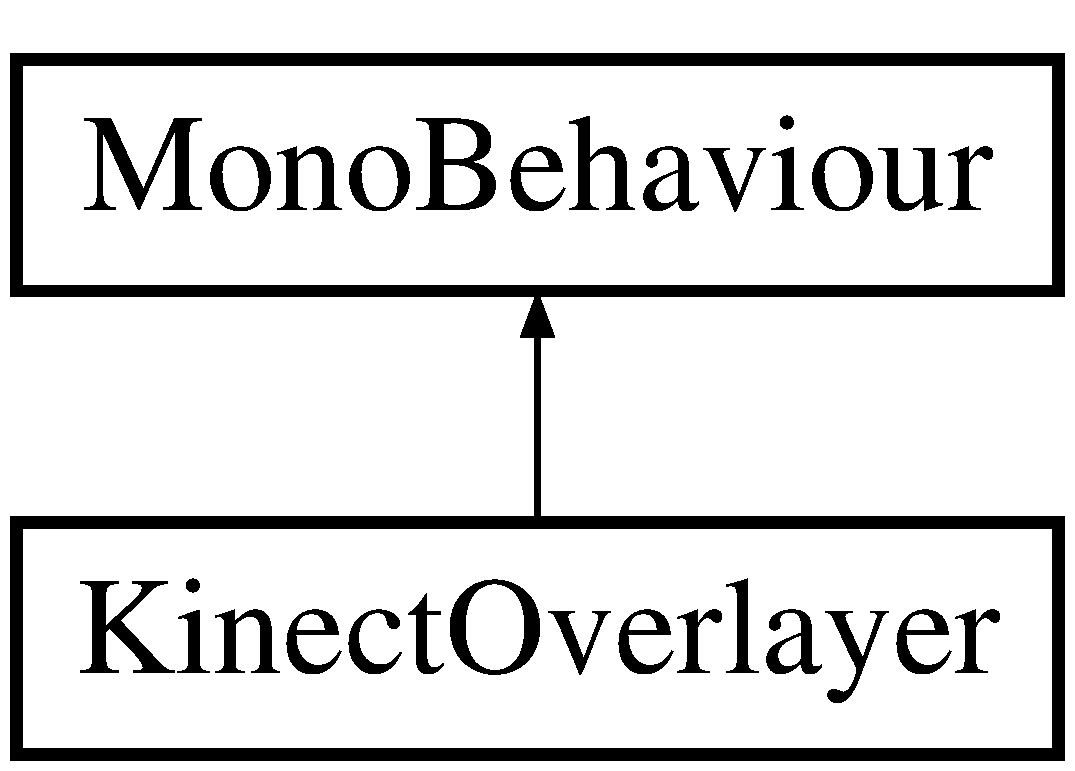
\includegraphics[height=2.000000cm]{class_kinect_overlayer}
\end{center}
\end{figure}
\subsection*{Public Attributes}
\begin{DoxyCompactItemize}
\item 
\mbox{\Hypertarget{class_kinect_overlayer_a800933f917e122ea689eea7dcf4b162e}\label{class_kinect_overlayer_a800933f917e122ea689eea7dcf4b162e}} 
G\+U\+I\+Texture {\bfseries background\+Image}
\item 
\mbox{\Hypertarget{class_kinect_overlayer_a269d0b0fb01f1b0e2ed8980c1e971d68}\label{class_kinect_overlayer_a269d0b0fb01f1b0e2ed8980c1e971d68}} 
Kinect\+Wrapper.\+Nui\+Skeleton\+Position\+Index {\bfseries Tracked\+Joint} = Kinect\+Wrapper.\+Nui\+Skeleton\+Position\+Index.\+Hand\+Right
\item 
\mbox{\Hypertarget{class_kinect_overlayer_ad7639e2eec99a29ab8b33a2467f331bd}\label{class_kinect_overlayer_ad7639e2eec99a29ab8b33a2467f331bd}} 
Game\+Object {\bfseries Overlay\+Object}
\item 
\mbox{\Hypertarget{class_kinect_overlayer_a49890aff78624a3501e063ed7269c757}\label{class_kinect_overlayer_a49890aff78624a3501e063ed7269c757}} 
float {\bfseries smooth\+Factor} = 5f
\item 
\mbox{\Hypertarget{class_kinect_overlayer_acb3b6a851b8cc6cc0e8c092dd279f99e}\label{class_kinect_overlayer_acb3b6a851b8cc6cc0e8c092dd279f99e}} 
G\+U\+I\+Text {\bfseries debug\+Text}
\end{DoxyCompactItemize}


The documentation for this class was generated from the following file\+:\begin{DoxyCompactItemize}
\item 
Assets/\+Overlay\+Demo/\+Scripts/Kinect\+Overlayer.\+cs\end{DoxyCompactItemize}

\hypertarget{class_kinect_wrapper}{}\section{Kinect\+Wrapper Class Reference}
\label{class_kinect_wrapper}\index{Kinect\+Wrapper@{Kinect\+Wrapper}}
\subsection*{Classes}
\begin{DoxyCompactItemize}
\item 
struct \mbox{\hyperlink{struct_kinect_wrapper_1_1_color_buffer}{Color\+Buffer}}
\item 
struct \mbox{\hyperlink{struct_kinect_wrapper_1_1_color_cust}{Color\+Cust}}
\item 
class {\bfseries Constants}
\item 
struct \mbox{\hyperlink{struct_kinect_wrapper_1_1_depth_buffer}{Depth\+Buffer}}
\item 
interface \mbox{\hyperlink{interface_kinect_wrapper_1_1_i_nui_frame_texture}{I\+Nui\+Frame\+Texture}}
\item 
class \mbox{\hyperlink{class_kinect_wrapper_1_1_nui_image_buffer}{Nui\+Image\+Buffer}}
\item 
struct \mbox{\hyperlink{struct_kinect_wrapper_1_1_nui_image_frame}{Nui\+Image\+Frame}}
\item 
struct \mbox{\hyperlink{struct_kinect_wrapper_1_1_nui_image_view_area}{Nui\+Image\+View\+Area}}
\item 
struct \mbox{\hyperlink{struct_kinect_wrapper_1_1_nui_locked_rect}{Nui\+Locked\+Rect}}
\item 
struct \mbox{\hyperlink{struct_kinect_wrapper_1_1_nui_skeleton_bone_orientation}{Nui\+Skeleton\+Bone\+Orientation}}
\item 
struct \mbox{\hyperlink{struct_kinect_wrapper_1_1_nui_skeleton_bone_rotation}{Nui\+Skeleton\+Bone\+Rotation}}
\item 
struct \mbox{\hyperlink{struct_kinect_wrapper_1_1_nui_skeleton_data}{Nui\+Skeleton\+Data}}
\item 
struct \mbox{\hyperlink{struct_kinect_wrapper_1_1_nui_skeleton_frame}{Nui\+Skeleton\+Frame}}
\item 
struct \mbox{\hyperlink{struct_kinect_wrapper_1_1_nui_surface_desc}{Nui\+Surface\+Desc}}
\item 
struct \mbox{\hyperlink{struct_kinect_wrapper_1_1_nui_transform_smooth_parameters}{Nui\+Transform\+Smooth\+Parameters}}
\end{DoxyCompactItemize}
\subsection*{Public Types}
\begin{DoxyCompactItemize}
\item 
enum \mbox{\hyperlink{class_kinect_wrapper_aa14891c91bfa8c6fe4761146055656da}{Nui\+Initialize\+Flags}} \+: uint \{ \newline
{\bfseries Uses\+Audio} = 0x10000000, 
{\bfseries Uses\+Depth\+And\+Player\+Index} = 0x00000001, 
{\bfseries Uses\+Color} = 0x00000002, 
{\bfseries Uses\+Skeleton} = 0x00000008, 
\newline
{\bfseries Uses\+Depth} = 0x00000020, 
{\bfseries Uses\+High\+Quality\+Color} = 0x00000040
 \}
\begin{DoxyCompactList}\small\item\em Structs and constants for interfacing C\# with the Kinect.\+dll \end{DoxyCompactList}\item 
\mbox{\Hypertarget{class_kinect_wrapper_a556dfab4f288c786036c4a48c5a57799}\label{class_kinect_wrapper_a556dfab4f288c786036c4a48c5a57799}} 
enum {\bfseries Nui\+Error\+Codes} \+: uint \{ \newline
{\bfseries Frame\+No\+Data} = 0x83010001, 
{\bfseries Stream\+Not\+Enabled} = 0x83010002, 
{\bfseries Image\+Stream\+In\+Use} = 0x83010003, 
{\bfseries Frame\+Limit\+Exceeded} = 0x83010004, 
\newline
{\bfseries Feature\+Not\+Initialized} = 0x83010005, 
{\bfseries Device\+Not\+Genuine} = 0x83010006, 
{\bfseries Insufficient\+Bandwidth} = 0x83010007, 
{\bfseries Device\+Not\+Supported} = 0x83010008, 
\newline
{\bfseries Device\+In\+Use} = 0x83010009, 
{\bfseries Database\+Not\+Found} = 0x8301000D, 
{\bfseries Database\+Version\+Mismatch} = 0x8301000E, 
{\bfseries Hardware\+Feature\+Unavailable} = 0x8301000F, 
\newline
{\bfseries Device\+Not\+Connected} = 0x83010014, 
{\bfseries Device\+Not\+Ready} = 0x83010015, 
{\bfseries Skeletal\+Engine\+Busy} = 0x830100\+AA, 
{\bfseries Device\+Not\+Powered} = 0x8301027F
 \}
\item 
\mbox{\Hypertarget{class_kinect_wrapper_ad73682163ab4e6f554501574ab835f1c}\label{class_kinect_wrapper_ad73682163ab4e6f554501574ab835f1c}} 
enum {\bfseries Nui\+Skeleton\+Position\+Index} \+: int \{ \newline
{\bfseries Hip\+Center} = 0, 
{\bfseries Spine} = 1, 
{\bfseries Shoulder\+Center} = 2, 
{\bfseries Head} = 3, 
\newline
{\bfseries Shoulder\+Left} = 4, 
{\bfseries Elbow\+Left} = 5, 
{\bfseries Wrist\+Left} = 6, 
{\bfseries Hand\+Left} = 7, 
\newline
{\bfseries Shoulder\+Right} = 8, 
{\bfseries Elbow\+Right} = 9, 
{\bfseries Wrist\+Right} = 10, 
{\bfseries Hand\+Right} = 11, 
\newline
{\bfseries Hip\+Left} = 12, 
{\bfseries Knee\+Left} = 13, 
{\bfseries Ankle\+Left} = 14, 
{\bfseries Foot\+Left} = 15, 
\newline
{\bfseries Hip\+Right} = 16, 
{\bfseries Knee\+Right} = 17, 
{\bfseries Ankle\+Right} = 18, 
{\bfseries Foot\+Right} = 19, 
\newline
{\bfseries Count} = 20
 \}
\item 
\mbox{\Hypertarget{class_kinect_wrapper_a2aa1ef02e1edc9d3bcb5dc78cc41e173}\label{class_kinect_wrapper_a2aa1ef02e1edc9d3bcb5dc78cc41e173}} 
enum {\bfseries Nui\+Skeleton\+Position\+Tracking\+State} \{ {\bfseries Not\+Tracked} = 0, 
{\bfseries Inferred}, 
{\bfseries Tracked}
 \}
\item 
\mbox{\Hypertarget{class_kinect_wrapper_a9d527d2064187b8e50453a8fa4158e49}\label{class_kinect_wrapper_a9d527d2064187b8e50453a8fa4158e49}} 
enum {\bfseries Nui\+Skeleton\+Tracking\+State} \{ {\bfseries Not\+Tracked} = 0, 
{\bfseries Position\+Only}, 
{\bfseries Skeleton\+Tracked}
 \}
\item 
\mbox{\Hypertarget{class_kinect_wrapper_a0126bd0303d23d562566d2ae99927335}\label{class_kinect_wrapper_a0126bd0303d23d562566d2ae99927335}} 
enum {\bfseries Nui\+Image\+Type} \{ \newline
{\bfseries Depth\+And\+Player\+Index} = 0, 
{\bfseries Color}, 
{\bfseries Color\+Y\+UV}, 
{\bfseries Color\+Raw\+Y\+UV}, 
\newline
{\bfseries Depth}
 \}
\item 
\mbox{\Hypertarget{class_kinect_wrapper_acef333d357f10c9b9b2e623ac4238470}\label{class_kinect_wrapper_acef333d357f10c9b9b2e623ac4238470}} 
enum {\bfseries Nui\+Image\+Resolution} \{ \newline
{\bfseries resolution\+Invalid} = -\/1, 
{\bfseries resolution80x60} = 0, 
{\bfseries resolution320x240} = 1, 
{\bfseries resolution640x480} = 2, 
\newline
{\bfseries resolution1280x960} = 3
 \}
\item 
\mbox{\Hypertarget{class_kinect_wrapper_ac51a99482e85bf5ea85af0e7e3bb25bd}\label{class_kinect_wrapper_ac51a99482e85bf5ea85af0e7e3bb25bd}} 
enum {\bfseries Nui\+Image\+Stream\+Flags} \{ {\bfseries None} = 0x00000000, 
{\bfseries Supress\+No\+Frame\+Data} = 0x0001000, 
{\bfseries Enable\+Near\+Mode} = 0x00020000, 
{\bfseries Too\+Far\+Is\+Non\+Zero} = 0x0004000
 \}
\item 
\mbox{\Hypertarget{class_kinect_wrapper_a70fa40d94bc2a6e7bdfe7a07d26ee535}\label{class_kinect_wrapper_a70fa40d94bc2a6e7bdfe7a07d26ee535}} 
enum {\bfseries Frame\+Edges} \{ \newline
{\bfseries None} = 0, 
{\bfseries Right} = 1, 
{\bfseries Left} = 2, 
{\bfseries Top} = 4, 
\newline
{\bfseries Bottom} = 8
 \}
\end{DoxyCompactItemize}
\subsection*{Public Member Functions}
\begin{DoxyCompactItemize}
\item 
\mbox{\Hypertarget{class_kinect_wrapper_a2fdd21af7c89b1d15bb20c412577ac29}\label{class_kinect_wrapper_a2fdd21af7c89b1d15bb20c412577ac29}} 
static int {\bfseries Nui\+Initialize} (\mbox{\hyperlink{class_kinect_wrapper_aa14891c91bfa8c6fe4761146055656da}{Nui\+Initialize\+Flags}} dw\+Flags)
\item 
\mbox{\Hypertarget{class_kinect_wrapper_ab80346c061343035f00f42dc89bb6e2e}\label{class_kinect_wrapper_ab80346c061343035f00f42dc89bb6e2e}} 
static void {\bfseries Nui\+Shutdown} ()
\item 
\mbox{\Hypertarget{class_kinect_wrapper_ae6798571cfc956305dc31020c72bf7ce}\label{class_kinect_wrapper_ae6798571cfc956305dc31020c72bf7ce}} 
static int {\bfseries Nui\+Camera\+Elevation\+Set\+Angle} (int angle)
\item 
\mbox{\Hypertarget{class_kinect_wrapper_aaaf8d63c9fabe873fe171f3a3e5f7ec7}\label{class_kinect_wrapper_aaaf8d63c9fabe873fe171f3a3e5f7ec7}} 
static int {\bfseries Nui\+Camera\+Elevation\+Get\+Angle} (out int pl\+Angle\+Degrees)
\item 
\mbox{\Hypertarget{class_kinect_wrapper_ac026341b4cf4127a4a84b24fa5547e59}\label{class_kinect_wrapper_ac026341b4cf4127a4a84b24fa5547e59}} 
static int {\bfseries Nui\+Image\+Get\+Color\+Pixel\+Coordinates\+From\+Depth\+Pixel\+At\+Resolution} (Nui\+Image\+Resolution e\+Color\+Resolution, Nui\+Image\+Resolution e\+Depth\+Resolution, ref \mbox{\hyperlink{struct_kinect_wrapper_1_1_nui_image_view_area}{Nui\+Image\+View\+Area}} pc\+View\+Area, int l\+DepthX, int l\+DepthY, ushort s\+Depth\+Value, out int pl\+ColorX, out int pl\+ColorY)
\item 
\mbox{\Hypertarget{class_kinect_wrapper_a7d786c97adcf86b866e4c5233b63f5fd}\label{class_kinect_wrapper_a7d786c97adcf86b866e4c5233b63f5fd}} 
static int {\bfseries Nui\+Get\+Sensor\+Count} (out int p\+Count)
\item 
\mbox{\Hypertarget{class_kinect_wrapper_a3e8731807ba8636cd10ae1b8cc7a7e4f}\label{class_kinect_wrapper_a3e8731807ba8636cd10ae1b8cc7a7e4f}} 
static int {\bfseries Nui\+Skeleton\+Tracking\+Enable} (Int\+Ptr h\+Next\+Frame\+Event, uint dw\+Flags)
\item 
\mbox{\Hypertarget{class_kinect_wrapper_a07d73b189c89e8f98ee9e03623b95de3}\label{class_kinect_wrapper_a07d73b189c89e8f98ee9e03623b95de3}} 
static int {\bfseries Nui\+Skeleton\+Get\+Next\+Frame} (uint dw\+Milliseconds\+To\+Wait, ref \mbox{\hyperlink{struct_kinect_wrapper_1_1_nui_skeleton_frame}{Nui\+Skeleton\+Frame}} p\+Skeleton\+Frame)
\item 
\mbox{\Hypertarget{class_kinect_wrapper_ab6c258db8ad4d3927af93397450ac30f}\label{class_kinect_wrapper_ab6c258db8ad4d3927af93397450ac30f}} 
static int {\bfseries Nui\+Transform\+Smooth} (ref \mbox{\hyperlink{struct_kinect_wrapper_1_1_nui_skeleton_frame}{Nui\+Skeleton\+Frame}} p\+Skeleton\+Frame, ref \mbox{\hyperlink{struct_kinect_wrapper_1_1_nui_transform_smooth_parameters}{Nui\+Transform\+Smooth\+Parameters}} p\+Smoothing\+Params)
\item 
\mbox{\Hypertarget{class_kinect_wrapper_a6aa2e92ea435aff8b2b529f9af865a17}\label{class_kinect_wrapper_a6aa2e92ea435aff8b2b529f9af865a17}} 
static int {\bfseries Nui\+Skeleton\+Calculate\+Bone\+Orientations} (ref \mbox{\hyperlink{struct_kinect_wrapper_1_1_nui_skeleton_data}{Nui\+Skeleton\+Data}} p\+Skeleton\+Data, \mbox{\hyperlink{struct_kinect_wrapper_1_1_nui_skeleton_bone_orientation}{Nui\+Skeleton\+Bone\+Orientation}}\mbox{[}$\,$\mbox{]} p\+Bone\+Orientations)
\item 
\mbox{\Hypertarget{class_kinect_wrapper_aa3d8db2048200771211ebf49f2e6ca47}\label{class_kinect_wrapper_aa3d8db2048200771211ebf49f2e6ca47}} 
static int {\bfseries Nui\+Image\+Stream\+Open} (Nui\+Image\+Type e\+Image\+Type, Nui\+Image\+Resolution e\+Resolution, uint dw\+Image\+Frame\+Flags\+\_\+\+Not\+Used, uint dw\+Frame\+Limit, Int\+Ptr h\+Next\+Frame\+Event, ref Int\+Ptr ph\+Stream\+Handle)
\item 
\mbox{\Hypertarget{class_kinect_wrapper_a85917a9af5cac4b8ea42756bb0f58a1a}\label{class_kinect_wrapper_a85917a9af5cac4b8ea42756bb0f58a1a}} 
static int {\bfseries Nui\+Image\+Stream\+Get\+Next\+Frame} (Int\+Ptr ph\+Stream\+Handle, uint dw\+Milliseconds\+To\+Wait, ref Int\+Ptr ppc\+Image\+Frame)
\item 
\mbox{\Hypertarget{class_kinect_wrapper_a881c04a93c8760da24c3e0d989675f7d}\label{class_kinect_wrapper_a881c04a93c8760da24c3e0d989675f7d}} 
static int {\bfseries Nui\+Image\+Stream\+Release\+Frame} (Int\+Ptr ph\+Stream\+Handle, Int\+Ptr ppc\+Image\+Frame)
\item 
\mbox{\Hypertarget{class_kinect_wrapper_aa781107969acc314e12407f42fd9a886}\label{class_kinect_wrapper_aa781107969acc314e12407f42fd9a886}} 
static int {\bfseries Nui\+Image\+Stream\+Set\+Image\+Frame\+Flags} (Int\+Ptr ph\+Stream\+Handle, Nui\+Image\+Stream\+Flags dv\+Image\+Frame\+Flags)
\item 
\mbox{\Hypertarget{class_kinect_wrapper_a387a5aef9e0ba9490e7c953acd662bf4}\label{class_kinect_wrapper_a387a5aef9e0ba9490e7c953acd662bf4}} 
static int {\bfseries Nui\+Image\+Resolution\+To\+Size} (Nui\+Image\+Resolution e\+Resolution, out uint frame\+Width, out uint frame\+Height)
\end{DoxyCompactItemize}
\subsection*{Static Public Member Functions}
\begin{DoxyCompactItemize}
\item 
\mbox{\Hypertarget{class_kinect_wrapper_a3cb502bd9f349d6ed93d318e27f96062}\label{class_kinect_wrapper_a3cb502bd9f349d6ed93d318e27f96062}} 
static string {\bfseries Get\+Nui\+Error\+String} (int hr)
\item 
\mbox{\Hypertarget{class_kinect_wrapper_afd77e6475589c7e610922ff3e0dc655c}\label{class_kinect_wrapper_afd77e6475589c7e610922ff3e0dc655c}} 
static int {\bfseries Get\+Depth\+Width} ()
\item 
\mbox{\Hypertarget{class_kinect_wrapper_a205e1fe831c2ea3eba4b46a0d3fbae73}\label{class_kinect_wrapper_a205e1fe831c2ea3eba4b46a0d3fbae73}} 
static int {\bfseries Get\+Depth\+Height} ()
\item 
\mbox{\Hypertarget{class_kinect_wrapper_a47574196fb217f80f0b4c348fc341758}\label{class_kinect_wrapper_a47574196fb217f80f0b4c348fc341758}} 
static int {\bfseries Get\+Color\+Width} ()
\item 
\mbox{\Hypertarget{class_kinect_wrapper_a06b0c509ebf20b8528616234edd3d4f6}\label{class_kinect_wrapper_a06b0c509ebf20b8528616234edd3d4f6}} 
static int {\bfseries Get\+Color\+Height} ()
\item 
\mbox{\Hypertarget{class_kinect_wrapper_a68f55b015fa7916f593a4a4a18f9537e}\label{class_kinect_wrapper_a68f55b015fa7916f593a4a4a18f9537e}} 
static Vector3 {\bfseries Map\+Skeleton\+Point\+To\+Depth\+Point} (Vector3 skeleton\+Point)
\item 
\mbox{\Hypertarget{class_kinect_wrapper_a206dc55a20ec2bdaa093df0b41ee81ad}\label{class_kinect_wrapper_a206dc55a20ec2bdaa093df0b41ee81ad}} 
static int {\bfseries Get\+Skeleton\+Joint\+Parent} (int joint\+Index)
\item 
\mbox{\Hypertarget{class_kinect_wrapper_a2e121255ab87d3ba7c442635f48c313c}\label{class_kinect_wrapper_a2e121255ab87d3ba7c442635f48c313c}} 
static int {\bfseries Get\+Skeleton\+Mirrored\+Joint} (int joint\+Index)
\item 
\mbox{\Hypertarget{class_kinect_wrapper_a013c4895027fa5c64eca7351d21f738c}\label{class_kinect_wrapper_a013c4895027fa5c64eca7351d21f738c}} 
static bool {\bfseries Poll\+Skeleton} (ref \mbox{\hyperlink{struct_kinect_wrapper_1_1_nui_transform_smooth_parameters}{Nui\+Transform\+Smooth\+Parameters}} smooth\+Parameters, ref \mbox{\hyperlink{struct_kinect_wrapper_1_1_nui_skeleton_frame}{Nui\+Skeleton\+Frame}} skeleton\+Frame)
\item 
\mbox{\Hypertarget{class_kinect_wrapper_a7432c928afbb7fae1bf3ed6b3efef0d7}\label{class_kinect_wrapper_a7432c928afbb7fae1bf3ed6b3efef0d7}} 
static bool {\bfseries Poll\+Color} (Int\+Ptr color\+Stream\+Handle, ref byte\mbox{[}$\,$\mbox{]} video\+Buffer, ref Color32\mbox{[}$\,$\mbox{]} color\+Image)
\item 
\mbox{\Hypertarget{class_kinect_wrapper_aa489e01c830842c81e6ecaa15d773efb}\label{class_kinect_wrapper_aa489e01c830842c81e6ecaa15d773efb}} 
static bool {\bfseries Poll\+Depth} (Int\+Ptr depth\+Stream\+Handle, bool is\+Near\+Mode, ref ushort\mbox{[}$\,$\mbox{]} depth\+Player\+Data)
\item 
\mbox{\Hypertarget{class_kinect_wrapper_a7afb7682da9118353458bb6c5c0c9636}\label{class_kinect_wrapper_a7afb7682da9118353458bb6c5c0c9636}} 
static void {\bfseries Get\+Skeleton\+Joint\+Orientation} (ref Vector3\mbox{[}$\,$\mbox{]} joints\+Pos, ref bool\mbox{[}$\,$\mbox{]} joints\+Tracked, ref Matrix4x4 \mbox{[}$\,$\mbox{]} joint\+Orients)
\end{DoxyCompactItemize}


\subsection{Member Enumeration Documentation}
\mbox{\Hypertarget{class_kinect_wrapper_aa14891c91bfa8c6fe4761146055656da}\label{class_kinect_wrapper_aa14891c91bfa8c6fe4761146055656da}} 
\index{Kinect\+Wrapper@{Kinect\+Wrapper}!Nui\+Initialize\+Flags@{Nui\+Initialize\+Flags}}
\index{Nui\+Initialize\+Flags@{Nui\+Initialize\+Flags}!Kinect\+Wrapper@{Kinect\+Wrapper}}
\subsubsection{\texorpdfstring{Nui\+Initialize\+Flags}{NuiInitializeFlags}}
{\footnotesize\ttfamily enum \mbox{\hyperlink{class_kinect_wrapper_aa14891c91bfa8c6fe4761146055656da}{Kinect\+Wrapper.\+Nui\+Initialize\+Flags}} \+: uint\hspace{0.3cm}{\ttfamily [strong]}}



Structs and constants for interfacing C\# with the Kinect.\+dll 



The documentation for this class was generated from the following file\+:\begin{DoxyCompactItemize}
\item 
Assets/\+Kinect\+Scripts/Kinect\+Wrapper.\+cs\end{DoxyCompactItemize}

\hypertarget{class_load_main_level}{}\section{Load\+Main\+Level Class Reference}
\label{class_load_main_level}\index{Load\+Main\+Level@{Load\+Main\+Level}}
Inheritance diagram for Load\+Main\+Level\+:\begin{figure}[H]
\begin{center}
\leavevmode
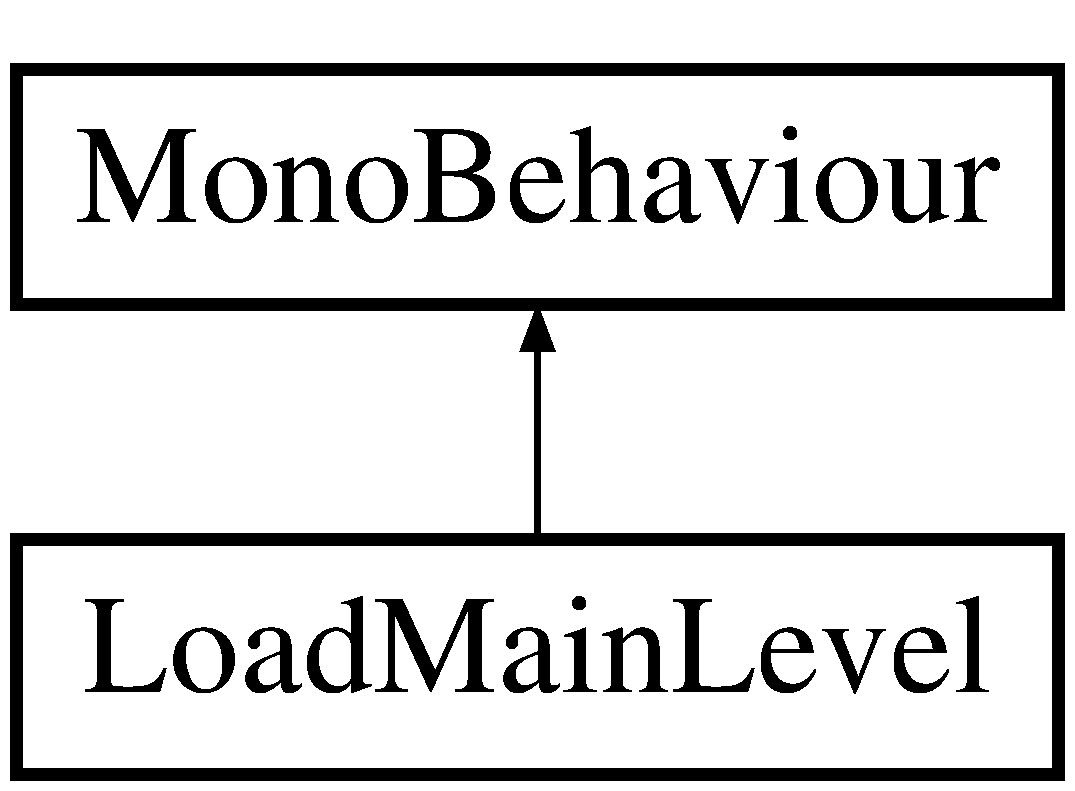
\includegraphics[height=2.000000cm]{class_load_main_level}
\end{center}
\end{figure}


The documentation for this class was generated from the following file\+:\begin{DoxyCompactItemize}
\item 
Assets/\+Kinect\+Scripts/\+Samples/Load\+Main\+Level.\+cs\end{DoxyCompactItemize}

\hypertarget{class_mouse_control}{}\section{Mouse\+Control Class Reference}
\label{class_mouse_control}\index{Mouse\+Control@{Mouse\+Control}}
\subsection*{Classes}
\begin{DoxyCompactItemize}
\item 
struct \mbox{\hyperlink{struct_mouse_control_1_1_r_e_c_t}{R\+E\+CT}}
\end{DoxyCompactItemize}
\subsection*{Static Public Member Functions}
\begin{DoxyCompactItemize}
\item 
\mbox{\Hypertarget{class_mouse_control_a800b976029f4f4999f3814fbc469ce94}\label{class_mouse_control_a800b976029f4f4999f3814fbc469ce94}} 
static void {\bfseries Mouse\+Move} (Vector3 screen\+Coordinates, G\+U\+I\+Text debug\+Text)
\item 
\mbox{\Hypertarget{class_mouse_control_afc4eeb0d38965242e550b97774f72cc6}\label{class_mouse_control_afc4eeb0d38965242e550b97774f72cc6}} 
static void {\bfseries Mouse\+Click} ()
\item 
\mbox{\Hypertarget{class_mouse_control_a7a4998be2c3f73acff61252d972d9f5e}\label{class_mouse_control_a7a4998be2c3f73acff61252d972d9f5e}} 
static void {\bfseries Mouse\+Drag} ()
\item 
\mbox{\Hypertarget{class_mouse_control_ad06284605529610482a31465b2f7f6b7}\label{class_mouse_control_ad06284605529610482a31465b2f7f6b7}} 
static void {\bfseries Mouse\+Release} ()
\end{DoxyCompactItemize}


The documentation for this class was generated from the following file\+:\begin{DoxyCompactItemize}
\item 
Assets/\+Kinect\+Scripts/\+Samples/Mouse\+Control.\+cs\end{DoxyCompactItemize}

\hypertarget{class_kinect_wrapper_1_1_nui_image_buffer}{}\section{Kinect\+Wrapper.\+Nui\+Image\+Buffer Class Reference}
\label{class_kinect_wrapper_1_1_nui_image_buffer}\index{Kinect\+Wrapper.\+Nui\+Image\+Buffer@{Kinect\+Wrapper.\+Nui\+Image\+Buffer}}
\subsection*{Public Attributes}
\begin{DoxyCompactItemize}
\item 
\mbox{\Hypertarget{class_kinect_wrapper_1_1_nui_image_buffer_a48b4d97b043d88cf5d17580e36c35e5d}\label{class_kinect_wrapper_1_1_nui_image_buffer_a48b4d97b043d88cf5d17580e36c35e5d}} 
int {\bfseries m\+\_\+\+Width}
\item 
\mbox{\Hypertarget{class_kinect_wrapper_1_1_nui_image_buffer_afd78a9db6894785383abbe65bb4be9eb}\label{class_kinect_wrapper_1_1_nui_image_buffer_afd78a9db6894785383abbe65bb4be9eb}} 
int {\bfseries m\+\_\+\+Height}
\item 
\mbox{\Hypertarget{class_kinect_wrapper_1_1_nui_image_buffer_a0291ec2dbbb18e55026c4c1e089e92bf}\label{class_kinect_wrapper_1_1_nui_image_buffer_a0291ec2dbbb18e55026c4c1e089e92bf}} 
int {\bfseries m\+\_\+\+Bytes\+Per\+Pixel}
\item 
\mbox{\Hypertarget{class_kinect_wrapper_1_1_nui_image_buffer_ae64fa64cd3f02ac5744ca189ac4570db}\label{class_kinect_wrapper_1_1_nui_image_buffer_ae64fa64cd3f02ac5744ca189ac4570db}} 
Int\+Ptr {\bfseries m\+\_\+p\+Buffer}
\end{DoxyCompactItemize}


The documentation for this class was generated from the following file\+:\begin{DoxyCompactItemize}
\item 
Assets/\+Kinect\+Scripts/Kinect\+Wrapper.\+cs\end{DoxyCompactItemize}

\hypertarget{struct_kinect_wrapper_1_1_nui_image_frame}{}\section{Kinect\+Wrapper.\+Nui\+Image\+Frame Struct Reference}
\label{struct_kinect_wrapper_1_1_nui_image_frame}\index{Kinect\+Wrapper.\+Nui\+Image\+Frame@{Kinect\+Wrapper.\+Nui\+Image\+Frame}}
\subsection*{Public Attributes}
\begin{DoxyCompactItemize}
\item 
\mbox{\Hypertarget{struct_kinect_wrapper_1_1_nui_image_frame_a956c4365ff4f5687b2c41ff96d1b03bc}\label{struct_kinect_wrapper_1_1_nui_image_frame_a956c4365ff4f5687b2c41ff96d1b03bc}} 
Int64 {\bfseries li\+Time\+Stamp}
\item 
\mbox{\Hypertarget{struct_kinect_wrapper_1_1_nui_image_frame_ad2060f260a57c7d2ffa1e46f660bc821}\label{struct_kinect_wrapper_1_1_nui_image_frame_ad2060f260a57c7d2ffa1e46f660bc821}} 
uint {\bfseries dw\+Frame\+Number}
\item 
\mbox{\Hypertarget{struct_kinect_wrapper_1_1_nui_image_frame_ada24f28ab364e7e338035897c79a2336}\label{struct_kinect_wrapper_1_1_nui_image_frame_ada24f28ab364e7e338035897c79a2336}} 
Nui\+Image\+Type {\bfseries e\+Image\+Type}
\item 
\mbox{\Hypertarget{struct_kinect_wrapper_1_1_nui_image_frame_a3b1994aae8d87c6125e866ee507c6d88}\label{struct_kinect_wrapper_1_1_nui_image_frame_a3b1994aae8d87c6125e866ee507c6d88}} 
Nui\+Image\+Resolution {\bfseries e\+Resolution}
\item 
\mbox{\Hypertarget{struct_kinect_wrapper_1_1_nui_image_frame_ad7bb8678b184d7b4e0184036b8808771}\label{struct_kinect_wrapper_1_1_nui_image_frame_ad7bb8678b184d7b4e0184036b8808771}} 
Int\+Ptr {\bfseries p\+Frame\+Texture}
\item 
\mbox{\Hypertarget{struct_kinect_wrapper_1_1_nui_image_frame_a2018d64c94f2316b50d55ab5749e3e6c}\label{struct_kinect_wrapper_1_1_nui_image_frame_a2018d64c94f2316b50d55ab5749e3e6c}} 
uint {\bfseries dw\+Frame\+Flags\+\_\+\+Not\+Used}
\item 
\mbox{\Hypertarget{struct_kinect_wrapper_1_1_nui_image_frame_a466d3e02ff63647b70017313652a0fb8}\label{struct_kinect_wrapper_1_1_nui_image_frame_a466d3e02ff63647b70017313652a0fb8}} 
\mbox{\hyperlink{struct_kinect_wrapper_1_1_nui_image_view_area}{Nui\+Image\+View\+Area}} {\bfseries View\+Area\+\_\+\+Not\+Used}
\end{DoxyCompactItemize}


The documentation for this struct was generated from the following file\+:\begin{DoxyCompactItemize}
\item 
Assets/\+Kinect\+Scripts/Kinect\+Wrapper.\+cs\end{DoxyCompactItemize}

\hypertarget{struct_kinect_wrapper_1_1_nui_image_view_area}{}\section{Kinect\+Wrapper.\+Nui\+Image\+View\+Area Struct Reference}
\label{struct_kinect_wrapper_1_1_nui_image_view_area}\index{Kinect\+Wrapper.\+Nui\+Image\+View\+Area@{Kinect\+Wrapper.\+Nui\+Image\+View\+Area}}
\subsection*{Public Attributes}
\begin{DoxyCompactItemize}
\item 
\mbox{\Hypertarget{struct_kinect_wrapper_1_1_nui_image_view_area_a56968a6e526e2e8700a6d0a996a039de}\label{struct_kinect_wrapper_1_1_nui_image_view_area_a56968a6e526e2e8700a6d0a996a039de}} 
int {\bfseries e\+Digital\+Zoom}
\item 
\mbox{\Hypertarget{struct_kinect_wrapper_1_1_nui_image_view_area_a903ae34c6272356bec3fdff63397a3eb}\label{struct_kinect_wrapper_1_1_nui_image_view_area_a903ae34c6272356bec3fdff63397a3eb}} 
int {\bfseries l\+CenterX}
\item 
\mbox{\Hypertarget{struct_kinect_wrapper_1_1_nui_image_view_area_a87a8110d362e3bcba5a37cfa13a00ead}\label{struct_kinect_wrapper_1_1_nui_image_view_area_a87a8110d362e3bcba5a37cfa13a00ead}} 
int {\bfseries l\+CenterY}
\end{DoxyCompactItemize}


The documentation for this struct was generated from the following file\+:\begin{DoxyCompactItemize}
\item 
Assets/\+Kinect\+Scripts/Kinect\+Wrapper.\+cs\end{DoxyCompactItemize}

\hypertarget{struct_kinect_wrapper_1_1_nui_locked_rect}{}\section{Kinect\+Wrapper.\+Nui\+Locked\+Rect Struct Reference}
\label{struct_kinect_wrapper_1_1_nui_locked_rect}\index{Kinect\+Wrapper.\+Nui\+Locked\+Rect@{Kinect\+Wrapper.\+Nui\+Locked\+Rect}}
\subsection*{Public Attributes}
\begin{DoxyCompactItemize}
\item 
\mbox{\Hypertarget{struct_kinect_wrapper_1_1_nui_locked_rect_a774555b91f90ec698409f3b6b02ec446}\label{struct_kinect_wrapper_1_1_nui_locked_rect_a774555b91f90ec698409f3b6b02ec446}} 
int {\bfseries pitch}
\item 
\mbox{\Hypertarget{struct_kinect_wrapper_1_1_nui_locked_rect_af9b113d7841ba06a110795fc37d600f0}\label{struct_kinect_wrapper_1_1_nui_locked_rect_af9b113d7841ba06a110795fc37d600f0}} 
int {\bfseries size}
\item 
\mbox{\Hypertarget{struct_kinect_wrapper_1_1_nui_locked_rect_a533926e413a6b88b40948bdcca58ba75}\label{struct_kinect_wrapper_1_1_nui_locked_rect_a533926e413a6b88b40948bdcca58ba75}} 
Int\+Ptr {\bfseries p\+Bits}
\end{DoxyCompactItemize}


The documentation for this struct was generated from the following file\+:\begin{DoxyCompactItemize}
\item 
Assets/\+Kinect\+Scripts/Kinect\+Wrapper.\+cs\end{DoxyCompactItemize}

\hypertarget{struct_kinect_wrapper_1_1_nui_skeleton_bone_orientation}{}\section{Kinect\+Wrapper.\+Nui\+Skeleton\+Bone\+Orientation Struct Reference}
\label{struct_kinect_wrapper_1_1_nui_skeleton_bone_orientation}\index{Kinect\+Wrapper.\+Nui\+Skeleton\+Bone\+Orientation@{Kinect\+Wrapper.\+Nui\+Skeleton\+Bone\+Orientation}}
\subsection*{Public Attributes}
\begin{DoxyCompactItemize}
\item 
\mbox{\Hypertarget{struct_kinect_wrapper_1_1_nui_skeleton_bone_orientation_ae04b67839d0c50106513eac6e4683e78}\label{struct_kinect_wrapper_1_1_nui_skeleton_bone_orientation_ae04b67839d0c50106513eac6e4683e78}} 
Nui\+Skeleton\+Position\+Index {\bfseries end\+Joint}
\item 
\mbox{\Hypertarget{struct_kinect_wrapper_1_1_nui_skeleton_bone_orientation_a040cf3d6ae0183a745da2bc3a854cd76}\label{struct_kinect_wrapper_1_1_nui_skeleton_bone_orientation_a040cf3d6ae0183a745da2bc3a854cd76}} 
Nui\+Skeleton\+Position\+Index {\bfseries start\+Joint}
\item 
\mbox{\Hypertarget{struct_kinect_wrapper_1_1_nui_skeleton_bone_orientation_aa668c0486f370e2f8a9d58ed59fae259}\label{struct_kinect_wrapper_1_1_nui_skeleton_bone_orientation_aa668c0486f370e2f8a9d58ed59fae259}} 
\mbox{\hyperlink{struct_kinect_wrapper_1_1_nui_skeleton_bone_rotation}{Nui\+Skeleton\+Bone\+Rotation}} {\bfseries hierarchical\+Rotation}
\item 
\mbox{\Hypertarget{struct_kinect_wrapper_1_1_nui_skeleton_bone_orientation_a65ae077aa43b08196177b17c2718aee9}\label{struct_kinect_wrapper_1_1_nui_skeleton_bone_orientation_a65ae077aa43b08196177b17c2718aee9}} 
\mbox{\hyperlink{struct_kinect_wrapper_1_1_nui_skeleton_bone_rotation}{Nui\+Skeleton\+Bone\+Rotation}} {\bfseries absolute\+Rotation}
\end{DoxyCompactItemize}


The documentation for this struct was generated from the following file\+:\begin{DoxyCompactItemize}
\item 
Assets/\+Kinect\+Scripts/Kinect\+Wrapper.\+cs\end{DoxyCompactItemize}

\hypertarget{struct_kinect_wrapper_1_1_nui_skeleton_bone_rotation}{}\section{Kinect\+Wrapper.\+Nui\+Skeleton\+Bone\+Rotation Struct Reference}
\label{struct_kinect_wrapper_1_1_nui_skeleton_bone_rotation}\index{Kinect\+Wrapper.\+Nui\+Skeleton\+Bone\+Rotation@{Kinect\+Wrapper.\+Nui\+Skeleton\+Bone\+Rotation}}
\subsection*{Public Attributes}
\begin{DoxyCompactItemize}
\item 
\mbox{\Hypertarget{struct_kinect_wrapper_1_1_nui_skeleton_bone_rotation_a2e27e61c545548e21cab9f1fe98b2fc5}\label{struct_kinect_wrapper_1_1_nui_skeleton_bone_rotation_a2e27e61c545548e21cab9f1fe98b2fc5}} 
Matrix4x4 {\bfseries rotation\+Matrix}
\item 
\mbox{\Hypertarget{struct_kinect_wrapper_1_1_nui_skeleton_bone_rotation_a9333030915c2c11562fd913873d8b4e1}\label{struct_kinect_wrapper_1_1_nui_skeleton_bone_rotation_a9333030915c2c11562fd913873d8b4e1}} 
Quaternion {\bfseries rotation\+Quaternion}
\end{DoxyCompactItemize}


The documentation for this struct was generated from the following file\+:\begin{DoxyCompactItemize}
\item 
Assets/\+Kinect\+Scripts/Kinect\+Wrapper.\+cs\end{DoxyCompactItemize}

\hypertarget{struct_kinect_wrapper_1_1_nui_skeleton_data}{}\section{Kinect\+Wrapper.\+Nui\+Skeleton\+Data Struct Reference}
\label{struct_kinect_wrapper_1_1_nui_skeleton_data}\index{Kinect\+Wrapper.\+Nui\+Skeleton\+Data@{Kinect\+Wrapper.\+Nui\+Skeleton\+Data}}
\subsection*{Public Attributes}
\begin{DoxyCompactItemize}
\item 
\mbox{\Hypertarget{struct_kinect_wrapper_1_1_nui_skeleton_data_a7614d2a370539c90ecb50c90fa6a23af}\label{struct_kinect_wrapper_1_1_nui_skeleton_data_a7614d2a370539c90ecb50c90fa6a23af}} 
Nui\+Skeleton\+Tracking\+State {\bfseries e\+Tracking\+State}
\item 
\mbox{\Hypertarget{struct_kinect_wrapper_1_1_nui_skeleton_data_a5d26d520d15dd02387ae88005582ddb4}\label{struct_kinect_wrapper_1_1_nui_skeleton_data_a5d26d520d15dd02387ae88005582ddb4}} 
uint {\bfseries dw\+Tracking\+ID}
\item 
\mbox{\Hypertarget{struct_kinect_wrapper_1_1_nui_skeleton_data_af7a43abd31650ea9ab62cf3dc42cb5f7}\label{struct_kinect_wrapper_1_1_nui_skeleton_data_af7a43abd31650ea9ab62cf3dc42cb5f7}} 
uint {\bfseries dw\+Enrollment\+Index\+\_\+\+Not\+Used}
\item 
\mbox{\Hypertarget{struct_kinect_wrapper_1_1_nui_skeleton_data_aa364897b7124bac16ac908be1f7d1d02}\label{struct_kinect_wrapper_1_1_nui_skeleton_data_aa364897b7124bac16ac908be1f7d1d02}} 
uint {\bfseries dw\+User\+Index}
\item 
\mbox{\Hypertarget{struct_kinect_wrapper_1_1_nui_skeleton_data_a04ade70ce81c5c2f6bb2b9e9b4594e81}\label{struct_kinect_wrapper_1_1_nui_skeleton_data_a04ade70ce81c5c2f6bb2b9e9b4594e81}} 
Vector4 {\bfseries Position}
\item 
\mbox{\Hypertarget{struct_kinect_wrapper_1_1_nui_skeleton_data_a022c731ef5e8d0df3673a137f4d9be4a}\label{struct_kinect_wrapper_1_1_nui_skeleton_data_a022c731ef5e8d0df3673a137f4d9be4a}} 
Vector4 \mbox{[}$\,$\mbox{]} {\bfseries Skeleton\+Positions}
\item 
\mbox{\Hypertarget{struct_kinect_wrapper_1_1_nui_skeleton_data_a9a7d78f99876e8973dd6ac8e0ea99817}\label{struct_kinect_wrapper_1_1_nui_skeleton_data_a9a7d78f99876e8973dd6ac8e0ea99817}} 
Nui\+Skeleton\+Position\+Tracking\+State \mbox{[}$\,$\mbox{]} {\bfseries e\+Skeleton\+Position\+Tracking\+State}
\item 
\mbox{\Hypertarget{struct_kinect_wrapper_1_1_nui_skeleton_data_a1b89a36bfe4139ff50ac3a1e26351098}\label{struct_kinect_wrapper_1_1_nui_skeleton_data_a1b89a36bfe4139ff50ac3a1e26351098}} 
uint {\bfseries dw\+Quality\+Flags}
\end{DoxyCompactItemize}


The documentation for this struct was generated from the following file\+:\begin{DoxyCompactItemize}
\item 
Assets/\+Kinect\+Scripts/Kinect\+Wrapper.\+cs\end{DoxyCompactItemize}

\hypertarget{struct_kinect_wrapper_1_1_nui_skeleton_frame}{}\section{Kinect\+Wrapper.\+Nui\+Skeleton\+Frame Struct Reference}
\label{struct_kinect_wrapper_1_1_nui_skeleton_frame}\index{Kinect\+Wrapper.\+Nui\+Skeleton\+Frame@{Kinect\+Wrapper.\+Nui\+Skeleton\+Frame}}
\subsection*{Public Attributes}
\begin{DoxyCompactItemize}
\item 
\mbox{\Hypertarget{struct_kinect_wrapper_1_1_nui_skeleton_frame_ae1a802eedfd2fa7734997aa6b50377df}\label{struct_kinect_wrapper_1_1_nui_skeleton_frame_ae1a802eedfd2fa7734997aa6b50377df}} 
Int64 {\bfseries li\+Time\+Stamp}
\item 
\mbox{\Hypertarget{struct_kinect_wrapper_1_1_nui_skeleton_frame_abb544866679b55667550df75368fd743}\label{struct_kinect_wrapper_1_1_nui_skeleton_frame_abb544866679b55667550df75368fd743}} 
uint {\bfseries dw\+Frame\+Number}
\item 
\mbox{\Hypertarget{struct_kinect_wrapper_1_1_nui_skeleton_frame_a462a1d2f769d87f08e6ff3433c0930f1}\label{struct_kinect_wrapper_1_1_nui_skeleton_frame_a462a1d2f769d87f08e6ff3433c0930f1}} 
uint {\bfseries dw\+Flags}
\item 
\mbox{\Hypertarget{struct_kinect_wrapper_1_1_nui_skeleton_frame_a23992f6462fa532b7c8a60379eb01e97}\label{struct_kinect_wrapper_1_1_nui_skeleton_frame_a23992f6462fa532b7c8a60379eb01e97}} 
Vector4 {\bfseries v\+Floor\+Clip\+Plane}
\item 
\mbox{\Hypertarget{struct_kinect_wrapper_1_1_nui_skeleton_frame_a5281e1a39eeda48cd88851cfcda6caf1}\label{struct_kinect_wrapper_1_1_nui_skeleton_frame_a5281e1a39eeda48cd88851cfcda6caf1}} 
Vector4 {\bfseries v\+Normal\+To\+Gravity}
\item 
\mbox{\Hypertarget{struct_kinect_wrapper_1_1_nui_skeleton_frame_ae130c1490c24b8354fb344989f556ade}\label{struct_kinect_wrapper_1_1_nui_skeleton_frame_ae130c1490c24b8354fb344989f556ade}} 
\mbox{\hyperlink{struct_kinect_wrapper_1_1_nui_skeleton_data}{Nui\+Skeleton\+Data}} \mbox{[}$\,$\mbox{]} {\bfseries Skeleton\+Data}
\end{DoxyCompactItemize}


The documentation for this struct was generated from the following file\+:\begin{DoxyCompactItemize}
\item 
Assets/\+Kinect\+Scripts/Kinect\+Wrapper.\+cs\end{DoxyCompactItemize}

\hypertarget{struct_kinect_wrapper_1_1_nui_surface_desc}{}\section{Kinect\+Wrapper.\+Nui\+Surface\+Desc Struct Reference}
\label{struct_kinect_wrapper_1_1_nui_surface_desc}\index{Kinect\+Wrapper.\+Nui\+Surface\+Desc@{Kinect\+Wrapper.\+Nui\+Surface\+Desc}}
\subsection*{Public Attributes}
\begin{DoxyCompactItemize}
\item 
\mbox{\Hypertarget{struct_kinect_wrapper_1_1_nui_surface_desc_a6b46bd248de10a081e430f5fc7c5113e}\label{struct_kinect_wrapper_1_1_nui_surface_desc_a6b46bd248de10a081e430f5fc7c5113e}} 
uint {\bfseries width}
\item 
\mbox{\Hypertarget{struct_kinect_wrapper_1_1_nui_surface_desc_a12cb7dbf93c38836a12d5e0b1909acbc}\label{struct_kinect_wrapper_1_1_nui_surface_desc_a12cb7dbf93c38836a12d5e0b1909acbc}} 
uint {\bfseries height}
\end{DoxyCompactItemize}


The documentation for this struct was generated from the following file\+:\begin{DoxyCompactItemize}
\item 
Assets/\+Kinect\+Scripts/Kinect\+Wrapper.\+cs\end{DoxyCompactItemize}

\hypertarget{struct_kinect_wrapper_1_1_nui_transform_smooth_parameters}{}\section{Kinect\+Wrapper.\+Nui\+Transform\+Smooth\+Parameters Struct Reference}
\label{struct_kinect_wrapper_1_1_nui_transform_smooth_parameters}\index{Kinect\+Wrapper.\+Nui\+Transform\+Smooth\+Parameters@{Kinect\+Wrapper.\+Nui\+Transform\+Smooth\+Parameters}}
\subsection*{Public Attributes}
\begin{DoxyCompactItemize}
\item 
\mbox{\Hypertarget{struct_kinect_wrapper_1_1_nui_transform_smooth_parameters_aa1bb9b319ef28e03be857f28555657d7}\label{struct_kinect_wrapper_1_1_nui_transform_smooth_parameters_aa1bb9b319ef28e03be857f28555657d7}} 
float {\bfseries f\+Smoothing}
\item 
\mbox{\Hypertarget{struct_kinect_wrapper_1_1_nui_transform_smooth_parameters_a7f6117cf078ffbed9c06c7324c5d28f1}\label{struct_kinect_wrapper_1_1_nui_transform_smooth_parameters_a7f6117cf078ffbed9c06c7324c5d28f1}} 
float {\bfseries f\+Correction}
\item 
\mbox{\Hypertarget{struct_kinect_wrapper_1_1_nui_transform_smooth_parameters_a5539423447d47867e98b526394e24f0d}\label{struct_kinect_wrapper_1_1_nui_transform_smooth_parameters_a5539423447d47867e98b526394e24f0d}} 
float {\bfseries f\+Prediction}
\item 
\mbox{\Hypertarget{struct_kinect_wrapper_1_1_nui_transform_smooth_parameters_a210636c91ed9be0ccca3d6dfd0d4e13c}\label{struct_kinect_wrapper_1_1_nui_transform_smooth_parameters_a210636c91ed9be0ccca3d6dfd0d4e13c}} 
float {\bfseries f\+Jitter\+Radius}
\item 
\mbox{\Hypertarget{struct_kinect_wrapper_1_1_nui_transform_smooth_parameters_a35a26e6f9d0df5110a080a80bdaaef55}\label{struct_kinect_wrapper_1_1_nui_transform_smooth_parameters_a35a26e6f9d0df5110a080a80bdaaef55}} 
float {\bfseries f\+Max\+Deviation\+Radius}
\end{DoxyCompactItemize}


The documentation for this struct was generated from the following file\+:\begin{DoxyCompactItemize}
\item 
Assets/\+Kinect\+Scripts/Kinect\+Wrapper.\+cs\end{DoxyCompactItemize}

\hypertarget{class_object_random_location}{}\section{Object\+Random\+Location Class Reference}
\label{class_object_random_location}\index{Object\+Random\+Location@{Object\+Random\+Location}}
Inheritance diagram for Object\+Random\+Location\+:\begin{figure}[H]
\begin{center}
\leavevmode
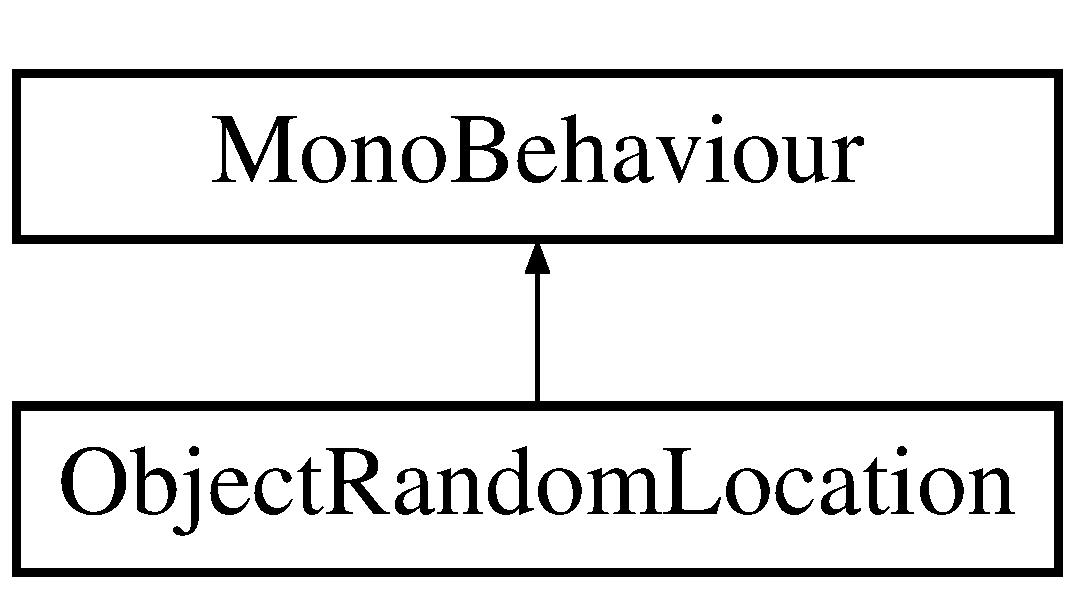
\includegraphics[height=2.000000cm]{class_object_random_location}
\end{center}
\end{figure}


The documentation for this class was generated from the following file\+:\begin{DoxyCompactItemize}
\item 
Assets/Object\+Random\+Location.\+cs\end{DoxyCompactItemize}

\hypertarget{class_presentation_script}{}\section{Presentation\+Script Class Reference}
\label{class_presentation_script}\index{Presentation\+Script@{Presentation\+Script}}
Inheritance diagram for Presentation\+Script\+:\begin{figure}[H]
\begin{center}
\leavevmode
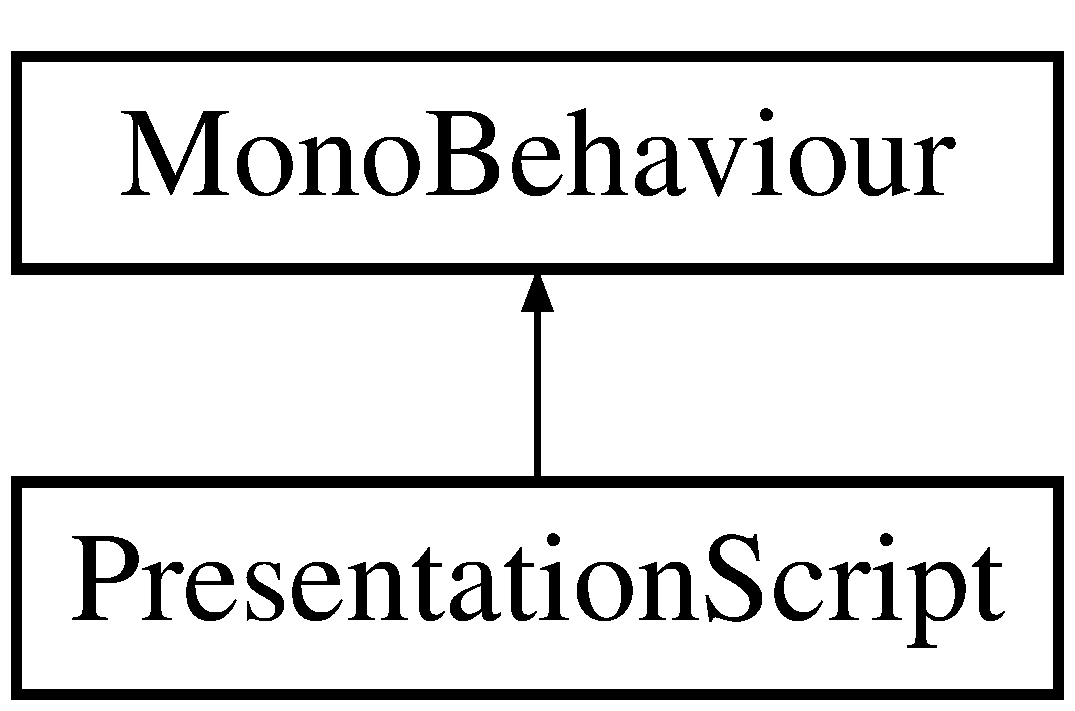
\includegraphics[height=2.000000cm]{class_presentation_script}
\end{center}
\end{figure}
\subsection*{Public Attributes}
\begin{DoxyCompactItemize}
\item 
\mbox{\Hypertarget{class_presentation_script_af4aad264ed181c135c3586eff805345b}\label{class_presentation_script_af4aad264ed181c135c3586eff805345b}} 
bool {\bfseries slide\+Change\+With\+Gestures} = true
\item 
\mbox{\Hypertarget{class_presentation_script_a30687753f5035843cdfa920a81ae15e9}\label{class_presentation_script_a30687753f5035843cdfa920a81ae15e9}} 
bool {\bfseries slide\+Change\+With\+Keys} = true
\item 
\mbox{\Hypertarget{class_presentation_script_af81c0a8a911a305f8a3aa269ce558181}\label{class_presentation_script_af81c0a8a911a305f8a3aa269ce558181}} 
float {\bfseries spin\+Speed} = 5
\item 
\mbox{\Hypertarget{class_presentation_script_ad88b126aebf1a294e12e897847d9e975}\label{class_presentation_script_ad88b126aebf1a294e12e897847d9e975}} 
bool {\bfseries auto\+Change\+Alfter\+Delay} = false
\item 
\mbox{\Hypertarget{class_presentation_script_a4aff472bbfc23c274b6da3d0172a8bb1}\label{class_presentation_script_a4aff472bbfc23c274b6da3d0172a8bb1}} 
float {\bfseries slide\+Change\+After\+Delay} = 10
\item 
\mbox{\Hypertarget{class_presentation_script_aedc1874d27439b88057822e0c8c3a00e}\label{class_presentation_script_aedc1874d27439b88057822e0c8c3a00e}} 
List$<$ Texture $>$ {\bfseries slide\+Textures}
\item 
\mbox{\Hypertarget{class_presentation_script_a2a2dd7e343b98335497e52061a41cd52}\label{class_presentation_script_a2a2dd7e343b98335497e52061a41cd52}} 
List$<$ Game\+Object $>$ {\bfseries horizontal\+Sides}
\item 
\mbox{\Hypertarget{class_presentation_script_ac6da9810878992688f780d61c7bb613c}\label{class_presentation_script_ac6da9810878992688f780d61c7bb613c}} 
bool {\bfseries is\+Behind\+User} = false
\end{DoxyCompactItemize}


The documentation for this class was generated from the following file\+:\begin{DoxyCompactItemize}
\item 
Assets/\+Gestures\+Demo/\+Scripts/Presentation\+Script.\+cs\end{DoxyCompactItemize}

\hypertarget{struct_mouse_control_1_1_r_e_c_t}{}\section{Mouse\+Control.\+R\+E\+CT Struct Reference}
\label{struct_mouse_control_1_1_r_e_c_t}\index{Mouse\+Control.\+R\+E\+CT@{Mouse\+Control.\+R\+E\+CT}}
\subsection*{Public Attributes}
\begin{DoxyCompactItemize}
\item 
\mbox{\Hypertarget{struct_mouse_control_1_1_r_e_c_t_a1aefdeec1cb3bd1222eaeb04713c5676}\label{struct_mouse_control_1_1_r_e_c_t_a1aefdeec1cb3bd1222eaeb04713c5676}} 
int {\bfseries Left}
\item 
\mbox{\Hypertarget{struct_mouse_control_1_1_r_e_c_t_a4f04a41b690fb8ca774c271deff0033b}\label{struct_mouse_control_1_1_r_e_c_t_a4f04a41b690fb8ca774c271deff0033b}} 
int {\bfseries Top}
\item 
\mbox{\Hypertarget{struct_mouse_control_1_1_r_e_c_t_a46b31f875cda8c248915e845398f83a1}\label{struct_mouse_control_1_1_r_e_c_t_a46b31f875cda8c248915e845398f83a1}} 
int {\bfseries Right}
\item 
\mbox{\Hypertarget{struct_mouse_control_1_1_r_e_c_t_a9a02216ee37790780949c85821fe69fe}\label{struct_mouse_control_1_1_r_e_c_t_a9a02216ee37790780949c85821fe69fe}} 
int {\bfseries Bottom}
\end{DoxyCompactItemize}


The documentation for this struct was generated from the following file\+:\begin{DoxyCompactItemize}
\item 
Assets/\+Kinect\+Scripts/\+Samples/Mouse\+Control.\+cs\end{DoxyCompactItemize}

\hypertarget{class_self_intersection_constraint}{}\section{Self\+Intersection\+Constraint Class Reference}
\label{class_self_intersection_constraint}\index{Self\+Intersection\+Constraint@{Self\+Intersection\+Constraint}}


Filter to prevent skeleton arm joints from intersecting the \char`\"{}body\char`\"{}.  


\subsection*{Public Member Functions}
\begin{DoxyCompactItemize}
\item 
\mbox{\Hypertarget{class_self_intersection_constraint_acf147bb20faea4fac58dc6f593588f44}\label{class_self_intersection_constraint_acf147bb20faea4fac58dc6f593588f44}} 
void {\bfseries Constrain} (ref \mbox{\hyperlink{struct_kinect_wrapper_1_1_nui_skeleton_data}{Kinect\+Wrapper.\+Nui\+Skeleton\+Data}} skeleton)
\end{DoxyCompactItemize}
\subsection*{Public Attributes}
\begin{DoxyCompactItemize}
\item 
\mbox{\Hypertarget{class_self_intersection_constraint_aa52dfc3119a99cd2cd5ef160906dcaa5}\label{class_self_intersection_constraint_aa52dfc3119a99cd2cd5ef160906dcaa5}} 
float {\bfseries Shoulder\+Extend} = 0.\+5f
\item 
\mbox{\Hypertarget{class_self_intersection_constraint_ac723559a2cd2b3f563b5b857b1357299}\label{class_self_intersection_constraint_ac723559a2cd2b3f563b5b857b1357299}} 
float {\bfseries Hip\+Extend} = 6.\+0f
\item 
\mbox{\Hypertarget{class_self_intersection_constraint_ac32f587ce2268e124021335b5d4d5338}\label{class_self_intersection_constraint_ac32f587ce2268e124021335b5d4d5338}} 
float {\bfseries Collision\+Tolerance} = 1.\+01f
\item 
\mbox{\Hypertarget{class_self_intersection_constraint_ac204dc28ae0a8e00165e46d64f4a5c78}\label{class_self_intersection_constraint_ac204dc28ae0a8e00165e46d64f4a5c78}} 
float {\bfseries Radius\+Multiplier} = 1.\+3f
\end{DoxyCompactItemize}


\subsection{Detailed Description}
Filter to prevent skeleton arm joints from intersecting the \char`\"{}body\char`\"{}. 



The documentation for this class was generated from the following file\+:\begin{DoxyCompactItemize}
\item 
Assets/\+Kinect\+Scripts/\+Filters/Self\+Intersection\+Constraint.\+cs\end{DoxyCompactItemize}

\hypertarget{class_set_scene_avatars}{}\section{Set\+Scene\+Avatars Class Reference}
\label{class_set_scene_avatars}\index{Set\+Scene\+Avatars@{Set\+Scene\+Avatars}}
Inheritance diagram for Set\+Scene\+Avatars\+:\begin{figure}[H]
\begin{center}
\leavevmode
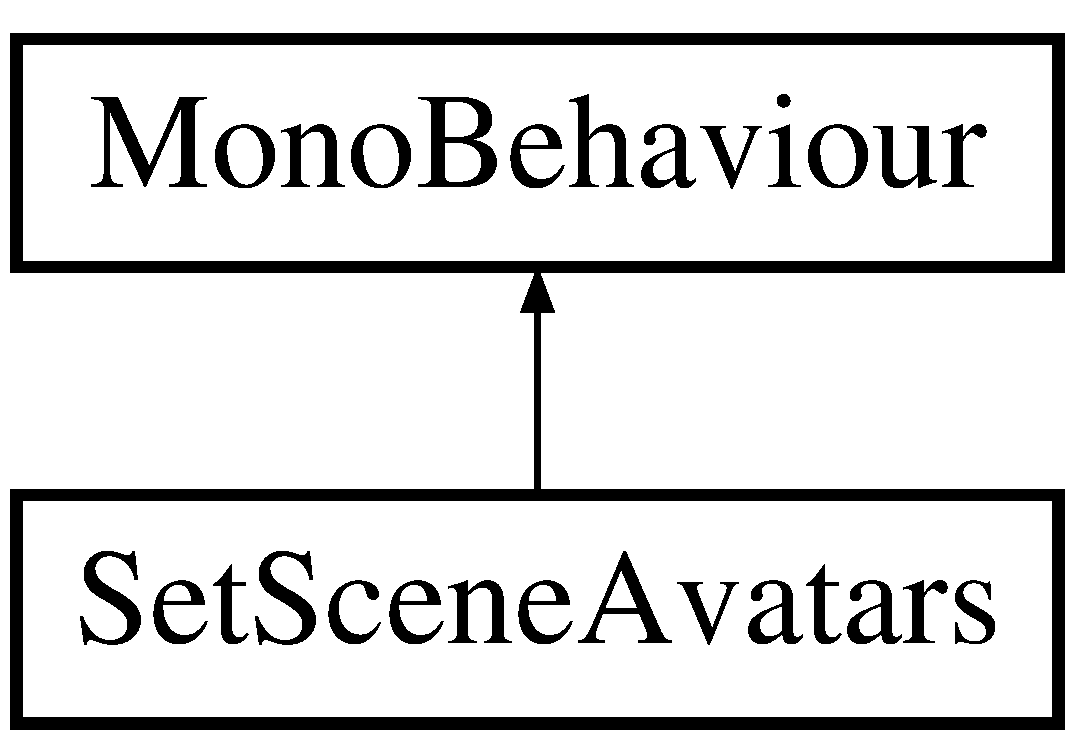
\includegraphics[height=2.000000cm]{class_set_scene_avatars}
\end{center}
\end{figure}


The documentation for this class was generated from the following file\+:\begin{DoxyCompactItemize}
\item 
Assets/\+Kinect\+Scripts/\+Samples/Set\+Scene\+Avatars.\+cs\end{DoxyCompactItemize}

\hypertarget{class_simple_gesture_listener}{}\section{Simple\+Gesture\+Listener Class Reference}
\label{class_simple_gesture_listener}\index{Simple\+Gesture\+Listener@{Simple\+Gesture\+Listener}}
Inheritance diagram for Simple\+Gesture\+Listener\+:\begin{figure}[H]
\begin{center}
\leavevmode
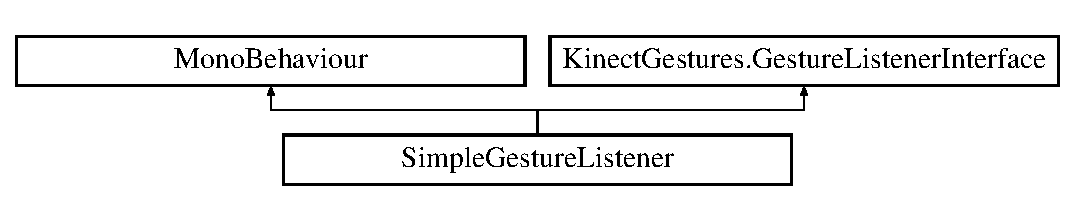
\includegraphics[height=2.000000cm]{class_simple_gesture_listener}
\end{center}
\end{figure}
\subsection*{Public Member Functions}
\begin{DoxyCompactItemize}
\item 
\mbox{\Hypertarget{class_simple_gesture_listener_a238368ecfe2e1b468fc1a9ad782f98f4}\label{class_simple_gesture_listener_a238368ecfe2e1b468fc1a9ad782f98f4}} 
void {\bfseries User\+Detected} (uint user\+Id, int user\+Index)
\item 
\mbox{\Hypertarget{class_simple_gesture_listener_a07c561adab62aaf1c1c3400658ebdeab}\label{class_simple_gesture_listener_a07c561adab62aaf1c1c3400658ebdeab}} 
void {\bfseries User\+Lost} (uint user\+Id, int user\+Index)
\item 
\mbox{\Hypertarget{class_simple_gesture_listener_a990029099c7e7bc9c45048ee0c10bf2f}\label{class_simple_gesture_listener_a990029099c7e7bc9c45048ee0c10bf2f}} 
void {\bfseries Gesture\+In\+Progress} (uint user\+Id, int user\+Index, Kinect\+Gestures.\+Gestures gesture, float progress, Kinect\+Wrapper.\+Nui\+Skeleton\+Position\+Index joint, Vector3 screen\+Pos)
\item 
\mbox{\Hypertarget{class_simple_gesture_listener_a72f86d012490f080a4334152757ce2e9}\label{class_simple_gesture_listener_a72f86d012490f080a4334152757ce2e9}} 
bool {\bfseries Gesture\+Completed} (uint user\+Id, int user\+Index, Kinect\+Gestures.\+Gestures gesture, Kinect\+Wrapper.\+Nui\+Skeleton\+Position\+Index joint, Vector3 screen\+Pos)
\item 
\mbox{\Hypertarget{class_simple_gesture_listener_ad65cddbc8d881020088b42edc9708434}\label{class_simple_gesture_listener_ad65cddbc8d881020088b42edc9708434}} 
bool {\bfseries Gesture\+Cancelled} (uint user\+Id, int user\+Index, Kinect\+Gestures.\+Gestures gesture, Kinect\+Wrapper.\+Nui\+Skeleton\+Position\+Index joint)
\end{DoxyCompactItemize}
\subsection*{Public Attributes}
\begin{DoxyCompactItemize}
\item 
\mbox{\Hypertarget{class_simple_gesture_listener_a39607eeb5fdd0e80d46d4a61fada2847}\label{class_simple_gesture_listener_a39607eeb5fdd0e80d46d4a61fada2847}} 
Text {\bfseries gesture\+Info}
\item 
\mbox{\Hypertarget{class_simple_gesture_listener_a40f39c51c72ea379efbce9a84156bb5a}\label{class_simple_gesture_listener_a40f39c51c72ea379efbce9a84156bb5a}} 
Game\+Object {\bfseries mercury}
\item 
\mbox{\Hypertarget{class_simple_gesture_listener_a04043c86a09bc4e4e844b003cc7892b2}\label{class_simple_gesture_listener_a04043c86a09bc4e4e844b003cc7892b2}} 
Game\+Object {\bfseries mars}
\item 
\mbox{\Hypertarget{class_simple_gesture_listener_aef0dd502d70df5beb875491cf97c2449}\label{class_simple_gesture_listener_aef0dd502d70df5beb875491cf97c2449}} 
Game\+Object {\bfseries venus}
\item 
\mbox{\Hypertarget{class_simple_gesture_listener_a46952f40626082a4b9284b537c7f859d}\label{class_simple_gesture_listener_a46952f40626082a4b9284b537c7f859d}} 
Game\+Object {\bfseries earth}
\item 
\mbox{\Hypertarget{class_simple_gesture_listener_ac3e1dc6250e8c99ec784952e17bdcef7}\label{class_simple_gesture_listener_ac3e1dc6250e8c99ec784952e17bdcef7}} 
Game\+Object {\bfseries jupiter}
\item 
\mbox{\Hypertarget{class_simple_gesture_listener_a5153012e62a475d247ca1f097da0d61a}\label{class_simple_gesture_listener_a5153012e62a475d247ca1f097da0d61a}} 
Game\+Object {\bfseries saturn}
\item 
\mbox{\Hypertarget{class_simple_gesture_listener_a609a50baf334b0a599b6b0fb0ecced17}\label{class_simple_gesture_listener_a609a50baf334b0a599b6b0fb0ecced17}} 
Game\+Object {\bfseries neptune}
\item 
\mbox{\Hypertarget{class_simple_gesture_listener_aa33da1e500332c8b2ced48906d461962}\label{class_simple_gesture_listener_aa33da1e500332c8b2ced48906d461962}} 
Game\+Object {\bfseries uranus}
\item 
\mbox{\Hypertarget{class_simple_gesture_listener_acfb3d06e489cc3e815cbcbaddcf9e939}\label{class_simple_gesture_listener_acfb3d06e489cc3e815cbcbaddcf9e939}} 
Game\+Object {\bfseries pluto}
\item 
\mbox{\Hypertarget{class_simple_gesture_listener_a496557f64816f7a44a0bd98df3d7d5c5}\label{class_simple_gesture_listener_a496557f64816f7a44a0bd98df3d7d5c5}} 
Game\+Object {\bfseries spaceship}
\end{DoxyCompactItemize}


The documentation for this class was generated from the following file\+:\begin{DoxyCompactItemize}
\item 
Assets/\+Kinect\+Scripts/\+Samples/Simple\+Gesture\+Listener.\+cs\end{DoxyCompactItemize}

\hypertarget{class_timed_lerp}{}\section{Timed\+Lerp Class Reference}
\label{class_timed_lerp}\index{Timed\+Lerp@{Timed\+Lerp}}


\mbox{\hyperlink{class_timed_lerp}{Timed\+Lerp}} -\/ Maintains a time-\/based lerp between 0 and a upper limit between 0 and 1. The lerp speed parameter is in units of inverse time -\/ therefore, a speed of 2.\+0 means that the lerp completes a full transition (0 to 1) in 0.\+5 seconds.  


\subsection*{Public Member Functions}
\begin{DoxyCompactItemize}
\item 
\mbox{\Hypertarget{class_timed_lerp_afd112ddd79c1dca6b8eed43fe8e8bf17}\label{class_timed_lerp_afd112ddd79c1dca6b8eed43fe8e8bf17}} 
void {\bfseries Set\+Speed} ()
\item 
\mbox{\Hypertarget{class_timed_lerp_a6a196647bd9dc81dedb9171b7a77ad75}\label{class_timed_lerp_a6a196647bd9dc81dedb9171b7a77ad75}} 
void \mbox{\hyperlink{class_timed_lerp_a6a196647bd9dc81dedb9171b7a77ad75}{Set\+Speed}} (float ease\+In\+Speed, float ease\+Out\+Speed)
\begin{DoxyCompactList}\small\item\em Set in/out speeds. \end{DoxyCompactList}\item 
\mbox{\Hypertarget{class_timed_lerp_aa3ea68ee9fc2e65a1b023b82f8104fd4}\label{class_timed_lerp_aa3ea68ee9fc2e65a1b023b82f8104fd4}} 
void {\bfseries Set\+Enabled} (bool is\+Enabled)
\item 
\mbox{\Hypertarget{class_timed_lerp_a6b0d6401a371c4596da83f3ba3379bdd}\label{class_timed_lerp_a6b0d6401a371c4596da83f3ba3379bdd}} 
void {\bfseries Set\+Enabled} (float enabled)
\item 
\mbox{\Hypertarget{class_timed_lerp_a6771a3babe6ccdc179962799b38a764f}\label{class_timed_lerp_a6771a3babe6ccdc179962799b38a764f}} 
void {\bfseries Reset} ()
\item 
\mbox{\Hypertarget{class_timed_lerp_a588b7b9530791c1b8b62a680423507ec}\label{class_timed_lerp_a588b7b9530791c1b8b62a680423507ec}} 
bool {\bfseries Is\+Enabled} ()
\item 
\mbox{\Hypertarget{class_timed_lerp_abfe1bf353d18a0fed4c9c83a665aa2fd}\label{class_timed_lerp_abfe1bf353d18a0fed4c9c83a665aa2fd}} 
bool \mbox{\hyperlink{class_timed_lerp_abfe1bf353d18a0fed4c9c83a665aa2fd}{Is\+Lerp\+Enabled}} ()
\begin{DoxyCompactList}\small\item\em Is\+Lerp\+Enabled reflects whether the current value is 0 or not. \end{DoxyCompactList}\item 
\mbox{\Hypertarget{class_timed_lerp_a16a1d4a28fb9a621808f94e877e4e518}\label{class_timed_lerp_a16a1d4a28fb9a621808f94e877e4e518}} 
void \mbox{\hyperlink{class_timed_lerp_a16a1d4a28fb9a621808f94e877e4e518}{Tick}} (float delta\+Time)
\begin{DoxyCompactList}\small\item\em Tick needs to be called once per frame. \end{DoxyCompactList}\end{DoxyCompactItemize}
\subsection*{Protected Attributes}
\begin{DoxyCompactItemize}
\item 
\mbox{\Hypertarget{class_timed_lerp_a38bd18cd8de9a62364e47bee6eb4771b}\label{class_timed_lerp_a38bd18cd8de9a62364e47bee6eb4771b}} 
float {\bfseries Enabled}
\item 
\mbox{\Hypertarget{class_timed_lerp_a3986137427e1e7bd66bb783fb2d86b10}\label{class_timed_lerp_a3986137427e1e7bd66bb783fb2d86b10}} 
float {\bfseries Value}
\item 
\mbox{\Hypertarget{class_timed_lerp_aeed2ea010b62bd529013dc9b9bcac0a7}\label{class_timed_lerp_aeed2ea010b62bd529013dc9b9bcac0a7}} 
float {\bfseries Ease\+In\+Speed}
\item 
\mbox{\Hypertarget{class_timed_lerp_a2a08436125e40b0c670c5fd90c7f6db9}\label{class_timed_lerp_a2a08436125e40b0c670c5fd90c7f6db9}} 
float {\bfseries Ease\+Out\+Speed}
\end{DoxyCompactItemize}
\subsection*{Properties}
\begin{DoxyCompactItemize}
\item 
\mbox{\Hypertarget{class_timed_lerp_a299ba73016b0b467b4e05f663da50c6e}\label{class_timed_lerp_a299ba73016b0b467b4e05f663da50c6e}} 
float {\bfseries Linear\+Value}\hspace{0.3cm}{\ttfamily  \mbox{[}get\mbox{]}}
\item 
\mbox{\Hypertarget{class_timed_lerp_aca0279f3da2195aa1c275a42e4694301}\label{class_timed_lerp_aca0279f3da2195aa1c275a42e4694301}} 
float {\bfseries Smooth\+Value}\hspace{0.3cm}{\ttfamily  \mbox{[}get\mbox{]}}
\end{DoxyCompactItemize}


\subsection{Detailed Description}
\mbox{\hyperlink{class_timed_lerp}{Timed\+Lerp}} -\/ Maintains a time-\/based lerp between 0 and a upper limit between 0 and 1. The lerp speed parameter is in units of inverse time -\/ therefore, a speed of 2.\+0 means that the lerp completes a full transition (0 to 1) in 0.\+5 seconds. 



The documentation for this class was generated from the following file\+:\begin{DoxyCompactItemize}
\item 
Assets/\+Kinect\+Scripts/\+Filters/Timed\+Lerp.\+cs\end{DoxyCompactItemize}

\hypertarget{class_tracking_state_filter}{}\section{Tracking\+State\+Filter Class Reference}
\label{class_tracking_state_filter}\index{Tracking\+State\+Filter@{Tracking\+State\+Filter}}


Implementation of a Holt Double Exponential Smoothing filter. The double exponential smooths the curve and predicts. There is also noise jitter removal.  


\subsection*{Public Member Functions}
\begin{DoxyCompactItemize}
\item 
\mbox{\Hypertarget{class_tracking_state_filter_a5b6bbc0762bd99b07d858927149f8e99}\label{class_tracking_state_filter_a5b6bbc0762bd99b07d858927149f8e99}} 
\mbox{\hyperlink{class_tracking_state_filter_a5b6bbc0762bd99b07d858927149f8e99}{Tracking\+State\+Filter}} ()
\begin{DoxyCompactList}\small\item\em Initializes a new instance of the class. \end{DoxyCompactList}\item 
\mbox{\Hypertarget{class_tracking_state_filter_a93adcb0571eed573d08d29df99c052d2}\label{class_tracking_state_filter_a93adcb0571eed573d08d29df99c052d2}} 
void {\bfseries Init} ()
\item 
void \mbox{\hyperlink{class_tracking_state_filter_a04be8b493efd27ca4e283194b0c88345}{Init}} (float smoothing\+Value, float correction\+Value, float prediction\+Value, float jitter\+Radius\+Value, float max\+Deviation\+Radius\+Value)
\begin{DoxyCompactList}\small\item\em Initialize the filter with a set of manually specified Transform\+Smooth\+Parameters. \end{DoxyCompactList}\item 
\mbox{\Hypertarget{class_tracking_state_filter_a94f28ab818af63dc0dbff981471b9155}\label{class_tracking_state_filter_a94f28ab818af63dc0dbff981471b9155}} 
void {\bfseries Init} (\mbox{\hyperlink{struct_kinect_wrapper_1_1_nui_transform_smooth_parameters}{Kinect\+Wrapper.\+Nui\+Transform\+Smooth\+Parameters}} smoothing\+Parameters)
\item 
\mbox{\Hypertarget{class_tracking_state_filter_aaebd55fd1665a15ec96813b24acee475}\label{class_tracking_state_filter_aaebd55fd1665a15ec96813b24acee475}} 
void {\bfseries Reset} ()
\item 
\mbox{\Hypertarget{class_tracking_state_filter_a32f3730ec7efc024aa0b3776634e5126}\label{class_tracking_state_filter_a32f3730ec7efc024aa0b3776634e5126}} 
void {\bfseries Update\+Filter} (ref \mbox{\hyperlink{struct_kinect_wrapper_1_1_nui_skeleton_data}{Kinect\+Wrapper.\+Nui\+Skeleton\+Data}} skeleton)
\end{DoxyCompactItemize}
\subsection*{Protected Member Functions}
\begin{DoxyCompactItemize}
\item 
\mbox{\Hypertarget{class_tracking_state_filter_a1893e102dd433941dc3dcd844f932ae4}\label{class_tracking_state_filter_a1893e102dd433941dc3dcd844f932ae4}} 
void {\bfseries Filter\+Joint} (ref \mbox{\hyperlink{struct_kinect_wrapper_1_1_nui_skeleton_data}{Kinect\+Wrapper.\+Nui\+Skeleton\+Data}} skeleton, int joint\+Index, ref \mbox{\hyperlink{struct_kinect_wrapper_1_1_nui_transform_smooth_parameters}{Kinect\+Wrapper.\+Nui\+Transform\+Smooth\+Parameters}} smoothing\+Parameters)
\end{DoxyCompactItemize}


\subsection{Detailed Description}
Implementation of a Holt Double Exponential Smoothing filter. The double exponential smooths the curve and predicts. There is also noise jitter removal. 



\subsection{Member Function Documentation}
\mbox{\Hypertarget{class_tracking_state_filter_a04be8b493efd27ca4e283194b0c88345}\label{class_tracking_state_filter_a04be8b493efd27ca4e283194b0c88345}} 
\index{Tracking\+State\+Filter@{Tracking\+State\+Filter}!Init@{Init}}
\index{Init@{Init}!Tracking\+State\+Filter@{Tracking\+State\+Filter}}
\subsubsection{\texorpdfstring{Init()}{Init()}}
{\footnotesize\ttfamily void Tracking\+State\+Filter.\+Init (\begin{DoxyParamCaption}\item[{float}]{smoothing\+Value,  }\item[{float}]{correction\+Value,  }\item[{float}]{prediction\+Value,  }\item[{float}]{jitter\+Radius\+Value,  }\item[{float}]{max\+Deviation\+Radius\+Value }\end{DoxyParamCaption})}



Initialize the filter with a set of manually specified Transform\+Smooth\+Parameters. 


\begin{DoxyParams}{Parameters}
{\em smoothing\+Value} & Smoothing = \mbox{[}0..1\mbox{]}, lower values is closer to the raw data and more noisy.\\
\hline
{\em correction\+Value} & Correction = \mbox{[}0..1\mbox{]}, higher values correct faster and feel more responsive.\\
\hline
{\em prediction\+Value} & Prediction = \mbox{[}0..n\mbox{]}, how many frames into the future we want to predict.\\
\hline
{\em jitter\+Radius\+Value} & Jitter\+Radius = The deviation distance in m that defines jitter.\\
\hline
{\em max\+Deviation\+Radius\+Value} & Max\+Deviation = The maximum distance in m that filtered positions are allowed to deviate from raw data.\\
\hline
\end{DoxyParams}


The documentation for this class was generated from the following file\+:\begin{DoxyCompactItemize}
\item 
Assets/\+Kinect\+Scripts/\+Filters/Tracking\+State\+Filter.\+cs\end{DoxyCompactItemize}

%--- End generated contents ---

% Index
\backmatter
\newpage
\phantomsection
\clearemptydoublepage
\addcontentsline{toc}{chapter}{Index}
\printindex

\end{document}
